\documentclass[11pt, openany]{book}
\usepackage[text={4.65in,7.45in}, centering, includefoot]{geometry}

\usepackage[table, x11names]{xcolor}
\usepackage{fontspec,realscripts}
\usepackage{polyglossia}

\usepackage{enumerate}
\pagestyle{plain}
\usepackage{fancyhdr}
\pagestyle{fancy}
\renewcommand{\headrulewidth}{0pt}
\usepackage{afterpage}
\usepackage{multirow}
\usepackage{amsmath}
\usepackage{amssymb}
\usepackage{graphicx}
\usepackage{longtable}
\usepackage{footnote}
\usepackage{perpage}
\MakePerPage{footnote}
%\usepackage{bigfoot}
%\DeclareNewFootnote[para]{default}
\usepackage{dblfnote}
\usepackage{xspace}
%\newcommand\nd{\textsuperscript{nd}\xspace}
\usepackage{array}
\usepackage{emptypage}

\usepackage{hyperref}   % Package for hyperlinks
\hypersetup{
colorlinks,
citecolor=black,
filecolor=black,
linkcolor=blue,
urlcolor=black
}

\usepackage[Devanagari, Latin]{ucharclasses}

\setdefaultlanguage{english}
\setotherlanguage{sanskrit}
\setmainfont[Scale=1]{Times New Roman}

\newfontfamily\s[Script=Devanagari, Scale=0.9]{Shobhika}
\newfontfamily\regular{Times New Roman}

\newcommand{\devanagarinumeral}[1]{%
	\devanagaridigits{\number \csname c@#1\endcsname}}

\setTransitionTo{Devanagari}{\s}
\setTransitionFrom{Devanagari}{\regular}

\XeTeXgenerateactualtext=1

\begin{document}
\thispagestyle{empty}
\begin{center}
{\large \textbf{NĀRĀYAṆA PAṆḌITA'S}}
\vspace{2mm}

{\Huge\textbf{BĪJAGAṆITĀVATAṂSA}}
\vspace{2mm}

{\Large\textbf{ PART I}}
\vspace{2mm}

{\large \textbf{श्री नारायणपण्डितविरचितः}}
\vspace{2mm}

{\Large \textbf{बीजगणितावतंसः}}
\vspace{2mm}

प्रथमो भागः
\vspace{10mm}

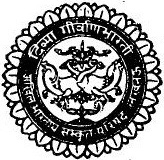
\includegraphics[scale=0.5]{fig1.jpeg}

\vspace{10mm}

{\small Critically Edited}
\vspace{2mm}

{\small by}
\vspace{2mm}

KRIPA SHANKAR SHUKLA

{\small Reader in Mathematics}

{\small University of Lucknow}
\vspace{40mm}

{\small \textit{Published by}}

\textbf{AKHILA BHARATIYA SANSKRIT PARISHAD}

{\small \textbf{LUCKNOW}}

{\small \textbf{1970}}
\end{center}

\newpage
\thispagestyle{empty}

\begin{center}
\textbf{C O N T E N T S}
\end{center}

\renewcommand*{\arraystretch}{1.5}
\begin{tabular}{llr}
 & & Pages \\
\hyperref[intro]{Introduction} & & i-iv \\
\textbf{बीजक्रियाभिधे पूर्वार्द्धे\textemdash} & &  \\
\hyperref[1]{उपक्रमः} & & १ \\
\hyperref[pari]{षट्त्रिंशत् परिकर्माणि} & & २-२८ \\
\hspace{5mm}{\small \hyperref[pari]{धनर्णषड्विधम्} (२-४)\,\textendash \,\hyperref[shu]{शून्यषड्विधम्}
(५-७)\,\textendash \,\hyperref[avy]{अव्यक्तषड्विधम्}} & &  \\
\hspace{5mm}{\small (७-१२)\,\textendash \,\hyperref[var]{वर्णषड्विधम्} (१२-१३)\,\textendash \,\hyperref[kar]{करणीषड्विधम्} (१३-२८)} & &  \\
\hyperref[kut]{कुट्टकः} & & २९-३५ \\
\hyperref[varga]{वर्गप्रकृतिः} & & ३६-४४ \\
\hspace{5mm}{\small \hyperref[varga]{वर्गप्रकृतिः} (३६-३८)\,\textendash \,\hyperref[cak]{चक्रवालम्} (३८-४०)\,\textendash \,\hyperref[81]{विशिष्टसूत्राणि} } & &  \\
\hspace{5mm}{\small (४०-४४)\,\textendash \,\hyperref[86]{आसन्नमूलानयनम्} (४४)} & &  \\
\textbf{बीजाभिधे उत्तरार्द्धे\textemdash} & &  \\
\hyperref[bij]{उपक्रमः} & & ४५ \\
\hyperref[3b]{अव्यक्तसाम्यं बीजम् (अपूर्णम्)} & & ४५-४६ 
\end{tabular}
\vspace{40mm}

\begin{center}
\textbf{ERRATA}
\end{center}

\begin{tabular}{lllllll}
Page & & Line & & Incorrect & & Correct \\
iii & & 19 & & निहितमना शारदायाः & & निहितमनाः शारदाया \\
1 & & 11 & & प्रश्ना न खिलीभिवन्ति & & प्रश्नानखिलीभवन्ति \\
32 & & 13 & & सम्भक्तो & & सप्तभक्तो \\
\end{tabular}
\afterpage{\fancyhead[RE]{{\small{ṚTAM}}}}
\afterpage{\fancyhead[LO]{{\small{NĀRĀYAṆA PAṆḌITA'S BĪJAGAṆITĀVATAṂSA}}}}
\afterpage{\fancyhead[LE,RO]{\thepage}}
\cfoot{}
\newpage
\pagenumbering{roman}
\thispagestyle{empty}

\phantomsection \label{intro}
\begin{center}
\textbf{INTRODUCTION}
\end{center}

The \textit{Bījagaṇitāvataṃsa} comes from the pen of Nārāyaṇa Paṇḍita and deals with algebra. The name \textit{Bījagaṇitāvataṃsa} is a compound formed by the composition of the words \textit{bījagaṇita}, meaning ``algebra" (lit. ``the science of calculation with elements"), and \textit{avataṃsa,}
meaning ``a garland or any ring-shaped ornament", or ``the crown." \textit{Bījagaṇitāvataṃsa} thus means ``a garland of the elements of algebra" or ``the crown of algebra".\\

Like other Hindu works on algebra, it is divided into two parts, Part I dealing with algebraic processes essential in solving algebraic equations (\textit{bījopa-yogi-gaṇita}) and Part II dealing with algebraic equations (\textit{bīja}). An incomplete manuscript of the work containing the whole of Part I and a few opening lines of Part II, which was acquired by the late Dr A. N. Singh, belongs to our collection. In the current issue of the \textit{Ṛtam} we propose to present a critically edited text of Part I. An English translation along with critical and explanatory notes will appear in a subsequent issue. Part II of the work is not available at present in its complete form and the reader will have to wait for it until a complete manuscript of the work is discovered.\\

Part I sets forth the following three topics:\\

(i) Algebraic operations (of addition, subtraction, multiplication, division, squaring and extracting the square root) for each of the following:
\vspace{2mm}

Positive \,and \,negative \,numbers \,(\textit{dhanarṇa}), \,the \,zero \,(\textit{śunya}), \,single unknown (\textit{avyakta}), more unknowns characterized by colours (\textit{varṇa}), and surds (\textit{karaṇī}).
\vspace{2mm}

(ii) The Pulverizer (\textit{kuṭṭaka}), i.e., analysis pertaining to the indeterminate equation $(ax \pm c)/b = y$.
\vspace{2mm}

(iii) The \,Square-nature \,(\textit{varga-prakṛti}), \,i.e., \,analysis \,pertaining \,to \,the indeterminate equation $Nx^2 \pm C = y^2$.\\

From the opening lines of Part II in our manuscript, we learn that it dealt as usual with the following algebraic equations (\textit{bīja}):\\

(i) Linear equations in one unknown (\textit{avyakta-samīkaraṇa}).
\newpage
(ii) Linear equations in more than one unknown (\textit{varṇa-samatva}).
\vspace{2mm}

(iii) Elimination of the middle term (\textit{madhyāmaharaṇa}), or the quadratic equation.
\vspace{2mm}

(iv) Equations \;involving \;the \;product \;of \;different \;unknowns (\textit{bhāvita-samatva}).\\

\noindent Our manuscript breaks off after giving the list of contents of Part II and an example of a linear equation in one unknown.\\

Part I ends with the following colophon giving the name of the author as Nārāyaṇa Paṇḍita and that of his father as Narasiṃha:\\

इति सकलकलानिधिनरसिंहनन्दन-गणितविद्याचतुरानन-श्रीनारायणपण्डितविरचिते
बीजगणितावतंसे वर्गप्रकृतिः समाप्ता~। \\

Comparison of this colophon with the following ones occurring at the ends of the \,various \,sections \,of \,the \,\textit{Gaṇitakaumudī} \,leaves \,little \,doubt \,that \,the author of the \textit{Bījagaṇitāvataṃsa} was the same Nārāyaṇa Paṇḍita as the author of \textit{Gaṇitakaumudī}.\\

(i) इति सकलकलानिधिनरसिंहनन्दन-गणितविद्याचतुरानन-श्रीनारायणपण्डितविर-चितायां गणितपाट्यां कौमुद्यां प्रकीर्णकानि समाप्तानि~।
\vspace{2mm}

(ii) इति सकलकलानिधिनरसिंहनन्दन-गणितविद्याचतुरानन-नारायणपण्डितविरचि-तायां गणितकौमुद्यां मिश्रव्यवहारः~।
\vspace{2mm}

(iii) इति सकलकलानिधिनरसिंहनन्दन-गणितविद्याचतुरानन-नारायणपण्डितविरचि-तायां गणितकौमुद्यां श्रेढीव्यवहारः~।
\vspace{2mm}

(iv) इति सकलकलानिधिनरसिंहनन्दन-गणितविद्याचतुरानन-नारायणपण्डितविरचि-तायां गणितपाट्यां कौमुद्याख्यायां श्रेत्रव्यवहारः समाप्तः~।
\vspace{2mm}

(v) इति सकलकलानिधिनरसिंहनन्दन-गणितविद्याचतुरानन-नारायणपण्डितविरचि-तायां गणितपाट्यां कौमुद्याख्यायां कुट्टको नाम नवमः व्यवहारः समाप्तः~।
\vspace{2mm}

(vi) इति श्रीसकलकलानिधिनरसिंहनन्दन-गणितविद्याचतुरानन-नारायणपण्डितविर-चितायां गणितपाट्यां कौमुद्याख्यायां वर्गप्रकृतिर्नाम दशमोऽध्यायः समाप्तः~।
\vspace{2mm}

(vii) इति श्रीसकलकलानिधिनरसिंहनन्दन-गणितविद्याचतुरानन-नारायणपण्डितवि-रचितायां गणितपाट्यां कौमुद्याख्यायां भागादानं नामैकादशो व्यवहारः समाप्तः~।

\newpage
(viii) \,इति \,श्रीसकलकलानिधिनरसिंहनन्दन-गणितविद्याचतुरानन-नारायणपण्डित-विरचितायां गणितपाट्यां कौमुद्याख्यायां रूपाद्यंशावतारो नाम द्वादशो व्यवहारः~।
\vspace{2mm}

(ix) इति श्रीसकलकलानिधिनरसिंहनन्दन-गणितविद्याचतुरानन-नारायणपण्डितवि-रचितायां गणितकौमुद्याख्यायामङ्कपाशो नाम त्रयोदशो व्यवहारः~।
\vspace{2mm}

(x) इति श्रीसकलकलानिधिश्रीमन्नृसिंहनन्दन-गणितविद्याचतुरानन-नारायणपण्डित-विरचितायां गणितपाट्यां भद्रगणितं नाम चतुर्दशो व्यवहारः~। \\

The \,identity \,of \,the \,authors \,of \,the \,\textit{Bījagaṇitāvataṃsa} \,and \,the \,\textit{Gaṇita-kaumudī} is also established by the fact that most of the verses (including commentaries thereon) found in the sections dealing with \textit{Kuṭṭaka} and \textit{Varga-prakṛti} in the two works are almost literally the same. There is also a reference in the \textit{Gaṇitakaumudī}\footnote{\textit{GK} (= \textit{Gaṇitakaumudī}), Part I, p. 13, lines 15-17.} to the author's \textit{Bījagaṇita}.\\

The following verse occurring in the end of the author's \textit{Gaṇitakaumudī} shows that the author's father Narasiṃha (Sk.\,Nṛsiṃha) was a respectable Brāhmaṇa well versed in the \textit{Śrutis} and \textit{Smṛtis} and a devotee of God Śiva; and that besides being a good scholar of the \textit{Śāstras}, he had acquired a high degree of proficiency in the mechanical science, the science of arms, and logic.

\begin{quote}
{\color{violet}आसीत् सौजन्यदुग्धाम्बुधिरवनिसुरश्रेणिमुख्यो जगत्यां\\
\emph{\color{white}अ} \hspace{4mm} प्रख्यः श्रीकण्ठपादद्वयनिहितमना शारदायाः निवासः~।\\
श्रौतस्मार्तार्थवेत्ता सकलगुणनिधिः शिल्पविद्याप्रगल्भः\\
\emph{\color{white}अ} \hspace{4mm} शास्त्रे शस्त्रे च तर्के प्रचुरतरगतिः श्रीनृसिंहो नृसिंहः~॥}\footnote{\textit{GK}, Part II, p. 410.}
\end{quote}

Nārāyaṇa Paṇḍita lived in the fourteenth century of
the Christian era. The following \,concluding \,verse \,of \,the \,\textit{Gaṇitakaumudī} \,shows \,that \,the \,\textit{Gaṇita-kaumudī} was completed on Thursday, the second \textit{tithi} of the dark fortnight of the month Kārtika, \textit{Saṃvatsara} Durmukha, \textit{Śaka} year 1278. This corresponds to Thursday, October 14, A.D. 1356. The \textit{Bījagaṇitāvataṃsa} which is mentioned in the \textit{Gaṇitakaumudī} was evidently written prior to this date.

\begin{quote}
{\color{violet}गजनगरविमितशाके दुर्मुखवर्षे च बाहुले मासि~।\\
धातृतिथौ कृष्णदले गुरौ समाप्तिं गतं गणितम्~॥}
\end{quote}
\vspace{12mm}

\newpage
The \textit{Gaṇitakaumudī} and the \textit{Bījagaṇitāvataṃsa} are the only two works on mathematics written by Nārāyaṇa Paṇḍita. The \textit{Gaṇitakaumudī} was edited by the late Padmakara Dvivedi and published in two parts, which appeared as No.\,57 (Part I) and No.\,57 (Part II) of the Princess of Wales Saraswati Bhavana Texts from Banaras in 1936 and 1942 respectively. Part I of the \textit{Bījagaṇitāvataṃsa} is being published now for the first time.\\

The above works show that their author Nārāyaṇa Paṇḍita was a good mathematician. He introduced new subjects of treatment and made his own contributions to the existing ones. He is the first mathematician to have dealt with the subject of "Magic Squares". Some  of his contributions are indeed remarkable and deserve special credit. In a paper entitled "Hindu methods for finding factors or divisors of a number"\footnote{\textit{Gaṇita}, Vol. 17, No. 2, 1966, pp. 101-109.} I have shown that the so called Fermat's factorization method was given by Nārāyaṇa in the \textit{Gaṇitakaumudī} about three centuries before it struck the mind of the French mathematician. There are quite a few problems which were proposed and solved for the first time by Nārāyaṇa. For example, mention may be made of the following:

\begin{quote}
{\color{violet}"A cow gives birth to a calf every year. The calves become young and themselves begin giving birth to calves when they are three years old. Tell me, O learned man, the number of progeny produced during twenty years by one cow."\footnote{\textit{GK}, Part I, p.126.}}
\end{quote}

One \,who \,goes \,through \,the \,present \,work \,will \,find \,that \,the \,alternative method for finding the square root of the surd\footnote{For a comparative study of the Hindu methods relating to surds, see A.\,N.\,Singh, "On the arithmetic of surds among the ancient Hindus," Mathematica, Vol. XII, 1936, pp. 102-115.} of the type $a + \sqrt{b} \,+ \sqrt{c} \,+ \sqrt{d}$ as given in Rule 46-49 and that for finding the approximate value of a quadratic surd as given in Rule 88 were given by Nārāyaṇa Paṇḍita for the first time.\\

I am grateful to Shri G.\,C.\,Sinha, Secretary, Akhila Bharatiya Sanskrit Parishad, Lucknow, for his keen interest in the present publication. My thanks are also due to Shri Markandeya Misra, Jyautishacharya, Research Assistant, Department of Mathematics and Astronomy, Lucknow University, for making this press copy of the manuscript.\\

\hfill \textbf{K. S. Shukla}

\newpage
\pagenumbering{arabic}
\thispagestyle{empty}
\begin{center}

\includegraphics[scale=0.7]{fig2.jpeg}
\vspace{8mm}

{\large{\textbf{श्रीनारायणपण्डितविरचितः}}}
\vspace{4mm}

{\Large{\textbf{बीजगणितावतंसः}}}
\vspace{2mm}

\rule{0.5\linewidth}{0.5pt}
\end{center}

\phantomsection \label{1}
\advance\leftmargini 4em \begin{quote}
\textbf{{\color{purple}एकमनेकस्योक्तं (नित्यं) व्यक्तस्य गुणवतो जगतः~।\\
गणनाविधेश्च बीजं ब्रह्म\renewcommand{\thefootnote}{१}\footnote{ब्रह्मे} च गणितं च तद्वन्दे~॥~१~॥}}\\

\textbf{{\color{purple}अजगोलोऽयमियानिति करकलितामलकसन्निभो येन~।\\
व्यक्तीचक्रे ह्यगणितगणितेन (च) तत् किमस्त्यन्यत्~॥~२~॥}}\\

\textbf{{\color{purple}गणितमिति नाम लोके ख्यातमभूदगणितस्य शास्त्रस्य~।\\
अगणितविक्रमविष्णोस्त्रिविक्रमश्चेति नामेव~॥~३~॥}}\\

\textbf{{\color{purple}सद्गुरुकृपयानुभवैरभ्यासैः परमतत्त्वमिव योगी~।\\
यो वेत्ति कर्म साङ्ख्यं स भवति सङ्ख्यावतां धुर्यः~॥~४~॥}}\\

\textbf{{\color{purple}यो यो यं यं प्रश्नं\renewcommand{\thefootnote}{२}\footnote{यं यः प्रश्नः~।} पृच्छति सम्यक्करणं न तस्यास्ति~।\\
व्यक्तेऽथाव्यक्ते तु प्रायस्तत्करणमस्त्येव\renewcommand{\thefootnote}{३}\footnote{मस्सेव~।}~॥~५~॥}}\\

\textbf{{\color{purple}व्यक्तक्रियया ज्ञातुं प्रश्ना न खिलीभिवन्ति\renewcommand{\thefootnote}{४}\footnote{ज्ञानुं प्रश्नान्यखी भ ।} नाल्पधियः~।\\
बीजक्रियां च तस्माद्वच्मि व्यक्तां सुबोधां च~॥~६~॥}}
\end{quote}
\vspace{28mm}

\afterpage{\fancyhead[RE]{{\small{ॠतम्}}}}
\afterpage{\fancyhead[LO]{{\small{श्रीनारायणपण्डितविरचितः बीजगणितावतंसः}}}}
\newpage
\renewcommand{\thepage}{\devanagarinumeral{page}}
\setcounter{page}{2}

\begin{center}
{\large{\textbf{[ बीजोपयोगिगणितम् ]}}}\\
\vspace{4mm}

\phantomsection \label{pari}
\textbf{(१) षट्त्रिंशत् परिकर्माणि}\\
\vspace{4mm}

(i) धनर्णषड्विधम्
\end{center}
\vspace{4mm}

धनर्ण\renewcommand{\thefootnote}{१}\footnote{धनार्ण~।}सङ्कलिते करणसूत्रमार्याद्वयम् \textendash 

\phantomsection \label{7}
\advance\leftmargini -4em \begin{quote}
\textbf{{\color{purple}रूपाणामव्यक्तानां नामाद्यक्षराणि लेख्यानि~।\\
उपलक्षणाय तेषामृणगानामूर्ध्वबिन्दुनि~॥~७~॥}}
\vspace{1mm}

\textbf{{\color{purple}योगे धनयोः क्षययोर्योगः स्यात् स्वर्णयोर्भवेद्विवरम्\renewcommand{\thefootnote}{२}\footnote{वर्णयो~।}~।\\
अधिकादूनमपास्य च शेषं तद्भावमुपयाति~॥~८~॥}}
\end{quote}

उदाहरणम् \textendash 

\begin{quote}
{\color{red}रूपत्रयञ्च रूपकपञ्चकमस्वं धनात्मकं वापि~।\\
वद सहितं झटिति सखे स्वर्णमृणं स्वं च यदि वेत्सि\renewcommand{\thefootnote}{३}\footnote{स्वर्णमृणं च यदि वेसि~।}~॥~१~॥}
\end{quote}

न्यासः\textendash \,रू ३ रू ५~। अत्र धनयोर्योगे योग इति योगे जातं रू ८~।
\vspace{2mm}

न्यासः\textendash \,रू $\dot{\hbox{३}}$ रू $\dot{\hbox{५}}$~। ॠणयोर्योगे योग इति जातं योगे रू $\dot{\hbox{८}}$~।
\vspace{2mm}

न्यासः\textendash \,रू ३ रू $\dot{\hbox{५}}$~। स्वर्णयोर्विवरमिति जातमृणभावं शेषं रू $\dot{\hbox{२}}$~। अयं योग एव~। 
\vspace{2mm}

न्यासः\textendash \,रू $\dot{\hbox{३}}$ रू ५~। स्वर्णयोर्विवरमिति जातं धनभावं शेषं रू २~। अयं योग एव~। एवं भिन्नेष्वपि~।

\begin{center}
इति धनर्णसङ्कलनम्~। 
\end{center}
\vspace{2mm}

धनर्णव्यवकलने सूत्रमार्यार्धम् \textendash 

\begin{quote}
\textbf{{\color{purple}स्वमृणत्वमृणं स्वत्वं शोधकराशेः समुक्तवद्योगः~।}}
\end{quote}

उदाहरणम् \textendash 

\begin{quote}
{\color{red}रूपाष्टकं रूपकपञ्चकेन\renewcommand{\thefootnote}{४}\footnote{रूपकं प ।}\\
\emph{\color{white}अ} \hspace{2mm} क्षयं क्षयेनापि धनं धनेन~।\\
धनं क्षयेण क्षयगं धनेन\\
\emph{\color{white}अ} \hspace{2mm} व्यस्तं च संशोध्य वदाशु\renewcommand{\thefootnote}{५}\footnote{वदाश्रु~।} शेषम्~॥~२~॥}
\end{quote}

\newpage

न्यासः\textendash \,रू $\dot{\hbox{८}}$ रू $\dot{\hbox{५}}$~। अत्र शोधके\renewcommand{\thefootnote}{१}\footnote{अत्र शोध अत्रशोधके~।} ऋणं स्वत्वमिति\renewcommand{\thefootnote}{२}\footnote{स्वमृणत्वमिति~।} जातं
स्वं रू $\dot{\hbox{८}}$ रू ५~। प्राग्वद्योगे जातं रू $\dot{\hbox{३}}$~। एतच्छेषम्~।
\vspace{2mm}

न्यासः\textendash \,रू ८ रू ५~। स्वमृणत्वमिति जातमृणत्वं रू ८ रू $\dot{\hbox{५}}$~। प्राग्वद्योगे जातं रू ३~।
\vspace{2mm}

न्यासः\textendash \,रू ८ रू $\dot{\hbox{५}}$~। ॠणं स्वत्वमिति जातं स्वं रू ८ रू ५~। प्राग्वद्योगः जातं रू १३~।
\vspace{2mm}

न्यासः\textendash \,रू $\dot{\hbox{८}}$ रू ५~।\renewcommand{\thefootnote}{३}\footnote{रू ८ रू ५~।} स्वमृणत्वमिति जातमृणत्वं रू $\dot{\hbox{८}}$ रू $\dot{\hbox{५}}$~। प्राग्वद्योगः रू $\dot{\hbox{१३}}$~। एतदन्तरम्~। 

\begin{center}
इति धनर्णव्यवकलना~। 
\end{center}
\vspace{2mm}

अथ धनर्णगुणने सूत्रमार्यार्धम् \textendash 

\begin{quote}
\textbf{{\color{purple}ॠणयोर्धनयोर्घाते स्वं स्यादृणधनहतावस्वम्~॥~९~॥}}
\end{quote}

उदाहरणम् \textendash 

\begin{quote}
{\color{red}रूपद्वयं रूपकपञ्चकेन\\
\emph{\color{white}अ} \hspace{2mm} धनं धनेन क्षयगं क्षयेण~।\\
धनं क्षयेण क्षयगं धनेन\\
\emph{\color{white}अ} \hspace{2mm} निघ्नं पृथक् किं गुणने फलं स्यात्~॥~३~॥}
\end{quote}

न्यासः\textendash \,रू २ रू ५ गुण्यगुणकौ\renewcommand{\thefootnote}{४}\footnote{गुणागुणकौ~।}~। धनयोर्घाते स्वं स्यादिति जातं रू १०~।
\vspace{2mm}

न्यासः\textendash \,रू $\dot{\hbox{२}}$ रू $\dot{\hbox{५}}$~। ॠणयोर्घाते\renewcommand{\thefootnote}{५}\footnote{योद्याते~।} स्वं स्यादिति जातं धनं रू १०~।
\vspace{2mm}

न्यासः\textendash \,रू २ रू $\dot{\hbox{५}}$~। ॠणधनहतावस्वमिति जातं रू $\dot{\hbox{१०}}$~। 
\vspace{2mm}

न्यासः\textendash \,रू $\dot{\hbox{२}}$ रू ५~। प्राग्वज्जातमृणं रू $\dot{\hbox{१०}}$~। एवं भिन्नेष्वपि~।
\vspace{2mm}

\begin{center}
इति धनर्णगुणना~। 
\end{center}
\vspace{2mm}

धनर्णभागहारे सूत्रम् \textendash 

\begin{quote}
\textbf{{\color{purple}ऋणधनगुणने यच्चोपलक्षणं तच्च भागहरणेऽपि~।}}
\end{quote}
\vspace{12mm}

\newpage

उदाहरणम् \textendash 

\begin{quote}
{\color{red}द्विनिघ्नरूपत्रितयं द्विकेन \\
\emph{\color{white}अ} \hspace{2mm} धनं धनेनर्णमृणेन भक्तम्\renewcommand{\thefootnote}{१}\footnote{धनं धनेनर्णम्~।}~। \\
ऋणं धनेन स्वमृणेन वापि \\
\emph{\color{white}अ} \hspace{2mm} सखे वदाश्वत्र\renewcommand{\thefootnote}{२}\footnote{दाश्च~।} हृतौ फलं मे~॥~४~॥}
\end{quote}

न्यासः\textendash \,रू ६ रू २~। अत्र गुणने\renewcommand{\thefootnote}{३}\footnote{नेन~।} यच्चोपलक्षणमिति यथा धनयोर्घाते धनं तथा धनयो-र्भजने धनमिति भागे हृते जातं रू ३~।
\vspace{2mm}

न्यासः\textendash \,रू${\dot{\hbox{ ६}}}$ रू ${\dot{\hbox{२}}}$~। भागे हृते जातं रू ३~। 
\vspace{2mm}

न्यासः\textendash \,रू ${\dot{\hbox{६}}}$ रू २~। गुणनवद् भागे हृते जातं रू ${\dot{\hbox{३}}}$~।
\vspace{2mm}

न्यासः\textendash \,रू ६ रू ${\dot{\hbox{२}}}$~। भागे हृते जातं रू ${\dot{\hbox{३}}}$~।

\begin{center}
इति धनर्णभागहारः~। 
\end{center}
\vspace{2mm}

धनर्णवर्गवर्गमूलयोः करणसूत्रम् \textendash 

\begin{quote}
\textbf{{\color{purple}ऋणधनयोश्च कृतिः स्वं धनमूलं धनमृणं भवेद्वापि~।\\
अकृतित्वादृणराशेर्मूलं नास्त्येव सिद्धमिति~॥~१०~॥}}
\end{quote}

उदाहरणम् \textendash 

\begin{quote}
{\color{red}सखे चतुर्णामधनात्मकानां\renewcommand{\thefootnote}{४}\footnote{मधुना~।}\\
\emph{\color{white}अ} \hspace{2mm} धनात्मकानाञ्च\renewcommand{\thefootnote}{५}\footnote{अनात्मकाना धनात्मका} कृतिं वदाशु\renewcommand{\thefootnote}{६}\footnote{दाश्रु~।}~।\\
धनस्य रूपद्विगुणाष्टकस्य \\
\emph{\color{white}अ} \hspace{2mm} क्षयस्य वा मित्र पृथक्पदं किम्~॥~५~॥}
\end{quote}

न्यासः\textendash \,रू ${\dot{\hbox{४}}}$, रू ४~। जातौ वर्गो १६, १६~।
\vspace{2mm}

न्यासः\textendash \,रू १६~। जातं मूलं रू ४, अथवा मूलं रू ${\dot{\hbox{४}}}$~।
\vspace{2mm}

न्यासः\textendash \,रू ${\dot{\hbox{१६}}}$~। अस्य क्षयगतस्य राशेरकृतित्वान्मूलं नास्तीति सिद्धम्~। 

\begin{center}
इति धनर्णवर्गमूले\renewcommand{\thefootnote}{७}\footnote{मुले~।}~।\\
\vspace{2mm}

इति धनर्णषड्विधम्~। 
\end{center}

\newpage

\phantomsection \label{shu}
\begin{center}
(ii) शून्यषड्विधम्
\end{center}

शून्यसङ्कलितव्यवकलितयोः करणसूत्रम्\textendash\,
\vspace{-1mm}

\phantomsection \label{11}
\begin{quote}
\textbf{{\color{purple}स्वर्ण\renewcommand{\thefootnote}{१}\footnote{स्वर्णं~।} शून्येन युतं विवर्जितं वा तथैव तद्भवति~।\\
शून्यादपनीतं तत् स्वर्णं व्यत्यासमुपयाति\renewcommand{\thefootnote}{२}\footnote{समुत्प~।}~॥~११~॥}}
\end{quote}

उदाहरणम् \textendash 
\vspace{-1mm}

\begin{quote}
{\color{red}रूपपञ्चकमृणं धनं सखे\\
\emph{\color{white}अ} \hspace{2mm} खेन युक्तमथवा विवर्जितम्~।\\
शून्यतः पृथगपास्य तानि वा\\
\emph{\color{white}अ} \hspace{2mm} किं भवेद् गणक मे पृथग्वद~॥~६~॥}
\end{quote}

न्यासः\renewcommand{\thefootnote}{३}\footnote{सेः न्यो~।}\textendash \,रू ${\dot{\hbox{५}}}$, रू ५~। एतानि खेन युतान्यूनितान्यविकृतानीव~।
\vspace{2mm}

न्यासः\textendash \,रू ${\dot{\hbox{५}}}$, रू ५~।  एतानि शून्यतश्च्युतानि जातानि व्यस्तानि\renewcommand{\thefootnote}{४}\footnote{व्यक्तानि~।} रू ५ रू ${\dot{\hbox{५}}}$,~।

\begin{center}
इति शून्यसंकलनव्यवकलने~। 
\end{center}
\vspace{2mm}

[ शून्यगुणने सूत्रमार्यार्धम्\renewcommand{\thefootnote}{५}\footnote{The portion enclosed within [ ] does not form part of the text. It is added to complete the text.} \textendash 

\begin{quote}
\textbf{{\color{purple}खं राशिना विगुणितं खं स्याद्राशिः खगुणश्च खं भवति~। }}
\end{quote}

उदाहरणम् \textendash 
\vspace{-1mm}

\begin{quote}
{\color{red}धनर्णभूतैस्त्रिभिरेव सङ्गुणं\\
\emph{\color{white}अ} \hspace{2mm} खं किं फलं स्यात्कथयाशु तन्मे~।\\
धनात्मकाश्चाप्यधनात्मकास्त्रयः \\
\emph{\color{white}अ} \hspace{2mm} खसंगुणाश्चापि फलं प्रचक्ष्व~॥~७~॥}
\end{quote}

न्यासः\textendash \,गुण्यः रू ०, गुणकः रू ३, रू${\dot{\hbox{ ३}}}$~। गुणने जातमुभयोः फलम् रू ०~।
\vspace{2mm}

न्यासः\textendash \,गुण्यः रू ३, रू ${\dot{\hbox{३}}}$~। गुणकः रू ०~। गणने जातमुभयोः फलम् रू ०~।

\begin{center}
इति शून्यगुणनाविधिः~। ]
\end{center}
\vspace{-1mm}

\newpage

शून्यभागहरणादौ सार्धमार्यासूत्रम् \textendash \\

खगुणादौ सूत्रम् \textendash 

\phantomsection \label{13}
\begin{quote}
\textbf{{\color{purple}खं राशिना विभक्तं खं स्याद्राशिः खभाजितः खहरः~॥~१२~॥ \\
शेषविधौ सति खगुणश्चिन्त्यः\renewcommand{\thefootnote}{१}\footnote{श्चित्यः~।} शून्ये गुणे खहारश्चेत्\renewcommand{\thefootnote}{२}\footnote{खहर~।}~।\\
पुनरेव तदाविकृतो राशिज्ञेयोऽत्र मतिमद्भिः~॥~१३~॥}}
\end{quote}

उदाहरणम् \textendash 

\begin{quote}
{\color{red}धनात्मकैश्चाप्यधनात्मकैस्त्रिभि-\\
\emph{\color{white}अ} \hspace{2mm} र्विभाजितं खं फलमाशु मे वद\renewcommand{\thefootnote}{३}\footnote{माश्रु वद~।}~। \\
धनात्मकाश्चाप्यधनात्म(का)स्त्रयः \\
\emph{\color{white}अ} \hspace{2mm} खभाजितास्त्वं गणक प्रवेत्सि चेत्~॥~७~॥}
\end{quote}

न्यासः\textendash \,भाज्यः रू ०, भाजकः रू ३, रू ${\dot{\hbox{३}}}$~। भागे हृते जातमुभयोः फलं ०~।
\vspace{2mm}

न्यासः\textendash \,भाज्यः रू ३, रू ${\dot{\hbox{३}}}$, भाजकः रू ०~। भागे हृते जातः खहरः रू ~{\scriptsize $\begin{matrix}
\vspace{-2mm}
\mbox{{३}}\\
\vspace{-1.5mm}
\mbox{{०}}
\vspace{1mm}
\end{matrix}$}~ रू ~{\scriptsize $\begin{matrix}
\vspace{-2mm}
{\dot{\hbox{३}}}\\
\vspace{-1.5mm}
\mbox{{०}}
\vspace{1mm}
\end{matrix}$}~।\renewcommand{\thefootnote}{४}\footnote{न्यासः भाज्यः रू उ भागे हृते जातः खहरः रू ३ वा रू २~।} \\

अत्र खहरगुण उच्यते \textendash 

\begin{quote}
\textbf{{\color{purple}शून्याभ्यासवशात्खतामुपगतो राशिः पुनः खोद्धृतो\\
व्यावृत्तिं पुनरेव तन्मयतया न प्राकृतिं गच्छति~। \\
आत्माभ्यासवशादनन्तममलं चिद्रूपमानन्ददं\renewcommand{\thefootnote}{५}\footnote{दनन्यममलं विद्रूपमानंददं~।} \\
प्राप्य\renewcommand{\thefootnote}{६}\footnote{प्राथ~।} ब्रह्मपदं न संसृतिपथं योगी गरीयानिव~॥~१४~॥}}
\end{quote}

प्राक्तनश्लोकश्च \textendash 

\begin{quote}
\textbf{{\color{purple}अस्मिन् विकारः खहरे न राशावपि प्रविष्टेष्वपि निःसृतेषु\renewcommand{\thefootnote}{७}\footnote{निःसृते तु~।}~।\\
\renewcommand{\thefootnote}{*}\footnote{This line is missing from the manuscript.}बहुष्वपि स्याल्लयसृष्टिकालेऽनन्तेऽच्युते भूतगणेषु यद्वत्~॥~१५~॥}}\renewcommand{\thefootnote}{८}\footnote{भास्करीयबीजगणिते\,शून्यषड्विधौ\,अंतिमश्लोकः\,।}
\end{quote}

\begin{center}
इति खरूपभागहारः~।
\end{center}

खयोग-वियोग-गुणन-भजन-वर्ग-वर्गमूलेषु सूत्रम् \textendash 

\begin{quote}
\textbf{{\color{purple}खं खयुतं रहितं वा खं स्यात् खेनाहतं च विहृतं वा~।\\
खस्य कृतिः खं खपदं खमेव सर्वत्र विज्ञेयम्~॥~१६~॥}}
\end{quote}

\newpage

उदाहरणम् \textendash 

\begin{quote}
{\color{red}खे शून्येन युते च किं विरहिते किं खेन निघ्ने च किं\\
\emph{\color{white}अ} \hspace{2mm} किं भक्ते किमु वर्गिते कथय भो मूलीकृते किं सखे ! \\
राशिः कोऽपि खसङ्गुणो निजदलेनाढ्यः\renewcommand{\thefootnote}{१}\footnote{विजदलेनाद्यः~।} खसंभाजितो\\
\emph{\color{white}अ} \hspace{2mm} जाता द्वादश तं द्रुतं\renewcommand{\thefootnote}{२}\footnote{छतं~।} वद दृढां प्रौढिं प्रयातोऽसि चेत्~॥~८~॥ }
\end{quote}

न्यासः\textendash \,रू ०~। एतत् खेन युतं जातं ०~। खेन रहितं जातं ०~। खेन गुणितं ०, भक्तं ०, वर्गितं ०, मूलीकृतम् ०~।\\

न्यासः\textendash \,०~। अज्ञातो राशिः कल्पितमिष्टं २~। अत्र '\hyperref[13]{शेषविधौ सति खगुणश्चिन्त्यः}' तत् कथम्\,? ० शून्येन द्विके गुणिते ०, अस्यार्द्धं ०, अनेन युतं ०, एतत् शून्येन हृतं शून्यमेव~। दृश्याभावादियं क्रिया न निर्वहति~। इष्टं २~। अत्र गणनायागतं शून्यं पृथङ् न्यस्तम्~। रू २, एतत्स्वार्धयुतं \,३~। भागहरणायागतं\renewcommand{\thefootnote}{३}\footnote{रणमागतं~।} \,शून्यं \,हरस्थाने \,न्यस्तम्~। शून्यं \,गुणकः \,शून्यं \,भागहा-रोऽतो गुणनभजने न कार्ये, तथाकृते जातोऽविकृतः ३~। यः कश्चिद् राशि: केनचिद् गुणितः पुनस्तेनैव भक्तश्चेदविकृत एव न भवति तर्हि गुणनभजने वृथा~। अथ तथाकृते जातं ३~। अत्र त्रैराशिकम्\textendash \,यदि दृश्येनानेन ३ अयं राशिः २ तदा द्वादशभिः किमिति जातो राशिः ८~।

\begin{center}
इति शून्यस्य षड्विधम्\renewcommand{\thefootnote}{४}\footnote{षड्विधे~।}~।
\vspace{4mm}

\phantomsection \label{avy}
(iii) अव्यक्तषड्विधम् ~~~~
\end{center}

अथाव्यक्तसङ्कलनव्यवकलने करणसूत्रम् \textendash 

\begin{quote}
\textbf{{\color{purple}यावत्तावत्-कालक-नीलक-पीताश्च लोहितो हरितः~। \\
श्वेतक-चित्रक-कपिलक-पाटलकाः पाण्डु-धूम्र-शबलाश्च~॥~१७~॥}}
\vspace{1mm}

\phantomsection \label{18}
\textbf{{\color{purple}श्यामलक-मेचक-धवलक-पिशङ्ग-शारङ्ग-बभ्रु-गौराद्याः~।\\
गणनोत्पत्त्यै विहिता संज्ञाश्चाव्यक्तमानानाम्~॥~१८~॥}}
\vspace{1mm}

\textbf{{\color{purple}वर्णेषु च समजात्योर्योगः कार्यस्तथा वियोगश्च~।\\ 
असदृशजात्योर्योगे पृथक्स्थितिः स्याद् वियोगे च~॥~१९~॥}}
\vspace{1mm}

\textbf{{\color{purple}क्षयधनयोर्युतिवियुती गुणनभजने वर्गवर्गमूले च~। \\
अव्यक्तानां बहूनां रूपवदुपलक्षणं भवति~॥~२०~॥}}
\end{quote}

गणनेति ~~योग-वियोग-गुणन-भजन-वर्ग-वर्गमूल-घन-घनमूल-त्रैराशिक-पंचराशिक- श्रेढि-क्षेत्र-खातादि यथोद्देशालापवत्त्वादेषां या \hyperref[18]{गणना} तस्या गणनाया\renewcommand{\thefootnote}{५}\footnote{णनया~।} \hyperref[18]{उत्पत्त्यै} अवताराय वर्णाः

\newpage

\noindent कल्पिताः~। ~~यावत्तावत्-\,कालक-\,नीलक-\,पीतक-\,लोहितक-\,हरितक-\,चित्रक-\,कपिलक- पाटलक-पाण्डुरक-\,धूम्रक-शबलक-श्यामलक-\,मेचक-धवलक-\,पिशङ्गक-सारङ्गक-बभ्रुक- गौरक इत्याद्या वर्णाः, अथवा वर्णाः कादयः, अथवा मधुरादयो\renewcommand{\thefootnote}{१}\footnote{मूधु~।} रसपर्यायाः, अथवा असदृ-शप्रथमाक्षरनामपदार्थाः कल्प्यन्ते~। एषु समजात्योर्बहूनां वा योगवियोगौ कार्यौ~। असदृश-जात्योर्बहूनां वा वर्णानां पृथक् स्थितिः स्यात्~। तेषां पर्यायानामप्युक्तानामृणधनयोगाद्युप-लक्षणं\renewcommand{\thefootnote}{२}\footnote{ते पर्यायषामद्युक्तानां ऋणधनयोगाद्रूपल~।} रूपवद्भवतीति~।\\

उदाहरणम् \textendash 

\begin{quote}
{\color{red}अव्यक्तषट्कं च धनं सरूप-\\
\emph{\color{white}अ} \hspace{2mm} मव्यक्तयुग्मञ्च विपञ्चरूपम्~।\\
किमेतयोरैक्यमृणं\renewcommand{\thefootnote}{३}\footnote{कि मेनयो~।} धनञ्च\\
\emph{\color{white}अ} \hspace{2mm} तद्व्यस्तयोः सङ्कलनं वदाशु\renewcommand{\thefootnote}{४}\footnote{दाश्रु~।}~॥~९~॥}
\end{quote}

न्यासः\textendash \,या ६ रू १ 
\vspace{2mm}

\hspace{10mm} या २ रू ${\dot{\hbox{५}}}$\\

\noindent समजात्योः स्वस्थाने योग इति जातं तथा न्यस्ते या ६ या २, रू १ रू ${\dot{\hbox{५}}}$~। ऋणधनयोः रूपवदुपलक्षणमिति\renewcommand{\thefootnote}{५}\footnote{दुपलक्षणलक्षण~।} योगे जातं या ८ रू ${\dot{\hbox{४}}}$~।\\

आद्यपक्षस्य ॠणत्वं प्रकल्प्य न्यासः \textendash 
\vspace{2mm}

\hspace{10mm} या ${\dot{\hbox{६}}}$ रू ${\dot{\hbox{१}}}$
\vspace{2mm}

\hspace{10mm} या २ रू ${\dot{\hbox{५}}}$
\vspace{2mm}

योगे जातं या${\dot{\hbox{ ४}}}$ रू${\dot{\hbox{ ६}}}$~। 
\vspace{2mm}

द्वितीयपक्षस्य वैपरीत्यं कृत्वा न्यासः \textendash 
\vspace{2mm}

\hspace{10mm} या ६ रू १ 
\vspace{2mm}

\hspace{10mm} या ${\dot{\hbox{२}}}$ रू ५ 
\vspace{2mm}

(योगे जातं) या ४ रू ६ 
\vspace{2mm}

उभयोर्व्यत्यासे न्यासः\textendash \,या ${\dot{\hbox{६}}}$ रू ${\dot{\hbox{१}}}$ 
\vspace{2mm}

\hspace{30mm} या${\dot{\hbox{ २}}}$ रू ५ 
\vspace{2mm}

योगे जातं या ${\dot{\hbox{८}}}$ रू ४~। 

\newpage

उदाहरणम् \textendash 

\begin{quote}
{\color{red}अव्यक्तवर्गद्वितयं सरूप-\\
\emph{\color{white}अ} \hspace{2mm} मव्यक्तयुग्मेन युतं च किं स्यात्~।\\
अव्यक्तषट्कं क्षयगं सरूपं \\
\emph{\color{white}अ} \hspace{2mm} शोध्यं तु षड्-रूपसु संयुतेभ्यः\renewcommand{\thefootnote}{१}\footnote{पसयु~।}~॥\\
अव्यक्तकेभ्यो गणक\,! प्रचक्ष्वा-\\
\emph{\color{white}अ} \hspace{2mm} ष्टाभ्योऽवशेषं यदि वेत्सि\renewcommand{\thefootnote}{२}\footnote{बेसि} बीजम्~॥~१०~॥}
\end{quote}

प्रथमोदाहरणे न्यासः \textendash 
\vspace{2mm}

\hspace{10mm} याव २ या ० रू १
\vspace{2mm}

\hspace{10mm} याव ० या २ रुः ०\\

योगे जातं याव २ या २ रू १~।\\

द्वितीयोदाहरणे न्यासः \textendash 
\vspace{2mm}

\hspace{10mm} या ८ रू ६ 
\vspace{2mm}

\hspace{10mm} या ${\dot{\hbox{६}}}$ रू १ \\

(वि)योगे जातं या १४ रू ५~।

\begin{center}
इत्यव्यक्तसंकलनव्यवकलने~। 
\end{center}
\vspace{2mm}

अथाव्यक्तगुणने करणसूत्रम् \textendash 

\begin{quote}
\textbf{{\color{purple}स्याद्रूपवर्णघाते\renewcommand{\thefootnote}{३}\footnote{स्याडूप~।} वर्णो, द्वित्र्यादितुल्यजातिवधे~। \\
तत्कृतिघनादयः स्युः\renewcommand{\thefootnote}{४}\footnote{स्यु~।} तद्भावितमसमजातिवधे~॥~२१~॥}}
\vspace{1mm}

\textbf{{\color{purple}गुणकारसमुत्थानि स्वजातिखण्डानि योजयेदेव\renewcommand{\thefootnote}{५}\footnote{देबे~।}~।\\
अव्यक्तवर्गकरणीगुणनासु व्यक्तवज्ज्ञेयम्\renewcommand{\thefootnote}{६}\footnote{वद्ज्ञे~।}~॥~२२~॥}}
\end{quote}
\vspace{12mm}

\newpage

उदाहरणम् \textendash 

\begin{quote}
{\color{red}यावत्तावद्द्वितयसहितं रूपषट्कं विनिघ्नं \\
\emph{\color{white}अ} \hspace{2mm} यावत्तावत्त्रितयरहितै\renewcommand{\thefootnote}{१}\footnote{द्द्वित~।} रूपकैः पञ्चभिश्च\renewcommand{\thefootnote}{२}\footnote{श्वंच~।}~।\\
गौणं किं स्याद् वद मम फलं हे सखे\,! कल्पयित्वा \\
\emph{\color{white}अ} \hspace{2mm} व्यक्ते वर्णे\renewcommand{\thefootnote}{३}\footnote{व्यक्तं वर्णं~।} पटुरसि यदि त्वं गुणाकारमार्गे~॥~११~॥}
\end{quote}

न्यासः \textendash 
\vspace{2mm}

\hspace{10mm} गुण्यः या २ रू ६
\vspace{2mm}

\hspace{10mm} गुणकः या${\dot{\hbox{ ३}}}$ रू ५\\

\noindent व्यक्तवद्गुणिते जातं याव ${\dot{\hbox{६}}}$ या ${\dot{\hbox{८}}}$ रू ३०~।\\

गुणकस्य धनर्णयोर्व्यत्यासे न्यासः \textendash 
\vspace{2mm}

\hspace{10mm} या २ रू ६
\vspace{2mm}

\hspace{10mm} या ३ रू ${\dot{\hbox{५}}}$\\

\noindent गुणिते जातं याव ६ या ८ रू ${\dot{\hbox{३०}}}$~। \\

गुण्यस्य व्यत्यासे न्यासः \textendash 
\vspace{2mm}

\hspace{10mm} या ${\dot{\hbox{२}}}$ रू ${\dot{\hbox{६}}}$
\vspace{2mm}

\hspace{10mm} या ${\dot{\hbox{३}}}$ रू ५\\

\noindent गुणिते जातं याव ६ या ८ रू ${\dot{\hbox{३०}}}$~।\renewcommand{\thefootnote}{४}\footnote{याव ६ या ${\dot{\hbox{८}}}$ रू ${\dot{\hbox{३०}}}$~।}\\

गुण्यगुणकयोर्व्यत्यासे न्यासः \textendash 
\vspace{2mm}

\hspace{10mm} या ${\dot{\hbox{२}}}$ रू ६
\vspace{2mm}

\hspace{10mm} या ३ रू ${\dot{\hbox{५}}}$\\

\noindent गुणिते जातं याव ${\dot{\hbox{६}}}$ या ${\dot{\hbox{८}}}$ रू ३०~।
\vspace{2mm}

\begin{center}
इत्यव्यक्तगुणना~। 
\end{center}

\newpage

अव्यक्तभागहारे सूत्रम् \textendash 

\begin{quote}
\textbf{{\color{purple}शुद्ध्यति यैर्यैर्वर्णै रूपैर्भाजको\renewcommand{\thefootnote}{१}\footnote{र्यै र्यैवर्णैरूप भा~।} हतो भाज्यात्~।\\
क्रमशः स्वेषु स्वेषु स्थानेषु फलानि तानि स्युः~॥~२३~॥}}
\end{quote}

गुणनफलस्य (= भाज्यस्य) गुण्यभागहारस्य भागार्थं\renewcommand{\thefootnote}{२}\footnote{गार्थ~।} न्यासः \textendash 
\vspace{2mm}

\begin{tabular}{lrlr}
(i) & याव ${\dot{\hbox{६}}}$ या ${\dot{\hbox{८}}}$ रू ३० & (ii) & याव ६ या ८ रू ${\dot{\hbox{३०}}}$ \\
 & या २ रू ६~~ &  & या २ रू ६~~ \\
(iii) & याव ६ या ८ रू ${\dot{\hbox{३०}}}$ & (iv) & याव ${\dot{\hbox{६}}}$ या ${\dot{\hbox{८}}}$ रू ३० \\
 & या ${\dot{\hbox{२}}}$ रू ${\dot{\hbox{६}}}$~ &  & या ${\dot{\hbox{२}}}$ रू ${\dot{\hbox{६}}}$~
\end{tabular}

\noindent भागे हृते जातो गुणः या ${\dot{\hbox{३}}}$ रू ५, या ३ रू ${\dot{\hbox{५}}}$, या ${\dot{\hbox{३}}}$ रू ५, या ३ रू ${\dot{\hbox{५}}}$~।

\begin{center}
इत्यव्यक्तभागहारः~।\renewcommand{\thefootnote}{३}\footnote{गहरः~।}
\end{center}

(अव्यक्तवर्गे उदाहरणम्\textendash\,)

\begin{quote}
{\color{red}अव्यक्तानां रूपपञ्चोनितानां \\
\emph{\color{white}अ} \hspace{2mm} षण्णां वर्गं वा युतानां प्रचक्ष्व~।\\
चेद्बीजज्ञोऽसि त्वमस्याः कृतेश्च\\
\emph{\color{white}अ} \hspace{2mm} मूलं विद्वन्\,! ब्रूहि तन्मे पृथक् किम्\renewcommand{\thefootnote}{४}\footnote{पृथः क्किं~।}~॥~१२~॥}
\end{quote}

न्यासः \textendash 

\hspace{10mm} या ६ रू${\dot{\hbox{ ५}}}$ 
\vspace{2mm}

\hspace{10mm} या ६ रू ५ \\

\noindent स्थाप्योऽन्त्यकृति\renewcommand{\thefootnote}{५}\footnote{स्थाथात्य~।}र्द्विसङ्गुणान्त्यगुणेत्यादिना जातौ वर्गौ \textendash 
\vspace{2mm}

\hspace{10mm} याव ३६ या${\dot{\hbox{ ६०}}}$ रू २५ 
\vspace{2mm}

\hspace{10mm} याव ३६ या ६० रू २५\\

(अव्यक्त वर्गमूले करण)सूत्रम् \textendash 

\begin{quote}
\textbf{{\color{purple}मूलान्यादायादौ वर्गेभ्यस्तद्द्वयोर्द्वयोर्घातम्\renewcommand{\thefootnote}{६}\footnote{द्वयोद्वयोधातं~।}~।\\
द्विगुणं\renewcommand{\thefootnote}{७}\footnote{द्विगुण~।} जह्याच्छेषान् मूलमितीदं वदन्तीह~॥~२४~॥}}
\end{quote}

\newpage

पूर्ववर्गमूलार्थं\renewcommand{\thefootnote}{१}\footnote{पूर्वंवर्गभूलार्थं~।} न्यासः\textendash\,
\vspace{2mm}

\hspace{9mm} याव ३६ या ${\dot{\hbox{६०}}}$ रू २५ 
\vspace{2mm}

\hspace{10mm} याव ३६ या ६० रू २५ \\

\noindent एतयोर्मूले या ६ रू ${\dot{\hbox{५}}}$~। या ६ रू ५~। 

\begin{center}
इत्यव्यक्तवर्गमूले~। 
\vspace{2mm}

इत्यव्यक्तषड्विधम्~।
\vspace{4mm}

\phantomsection \label{var}
(iv) वर्णषड्विधम् ~~~
\end{center}

उदाहरणम् \textendash 

\begin{quote}
{\color{red}यावत्तावत्त्रितयमधनं कालकाः षट् क्षयं भोः \\
\emph{\color{white}अ} \hspace{2mm} विद्वन्\,! नीलाष्टकमपि धनं पीतकाः स्वं च पञ्च~। \\
रूपाढ्यैस्तैर्द्विगुणितमितैस्तेऽपि युक्ता वियुक्ताः \\
\emph{\color{white}अ} \hspace{2mm} जानासि त्वं यदि झटिति मे ब्रूहि वर्णाः कति स्युः~॥~१३~॥}
\vspace{1mm}

{\color{red}तैस्तैर्हता\renewcommand{\thefootnote}{२}\footnote{तैस्तै हृता~।} कथय किं गुणने फलं स्याद् \\
\emph{\color{white}अ} \hspace{2mm} भक्तं\renewcommand{\thefootnote}{३}\footnote{भुक्तं~।} च तद्गणकवर्य\renewcommand{\thefootnote}{४}\footnote{गुणकवर्ग~।} गुणेन तेन~।\\
गुण्यस्य मे कथय वर्गमतश्च मूलं \\
\emph{\color{white}अ} \hspace{2mm} चेद्वर्णषड्विधविधाववधिं गतोऽसि~॥~१४~॥}
\end{quote}

न्यासः \textendash 
\vspace{2mm}

\hspace{10mm} या ${\dot{\hbox{३}}}$ का ${\dot{\hbox{६}}}$ नी ८ पी ५ रू १
\vspace{2mm}

\hspace{10mm} या ${\dot{\hbox{६}}}$ का ${\dot{\hbox{१२}}}$ नी १६ पी १० रू २\\

\noindent योगे जातम्\textendash \,या ${\dot{\hbox{९}}}$ का ${\dot{\hbox{१८}}}$ नी २४ पी १५ रू ३~। ~~वियोगे जातम्\textendash \,या ${\dot{\hbox{३}}}$ का ${\dot{\hbox{६}}}$ नी ८ पी ५ रू १~। 
\vspace{-2mm}

\begin{center}
इति वर्णसङ्कलनव्यवकलने~। 
\end{center}
\vspace{2mm}

(गुणने) न्यासः \textendash 
\vspace{2mm}

\hspace{10mm} गुण्यः ~~~या ${\dot{\hbox{३}}}$ का ${\dot{\hbox{६}}}$ नी ८ पी ५ रू १ 
\vspace{2mm}

\hspace{10mm} गुणकः ~या ${\dot{\hbox{६}}}$ का ${\dot{\hbox{१२}}}$ नी १६ पी १० रू २ 

\newpage

गुणिते जातम्\textendash \,याव १८ याका ७२ यानी ${\dot{\hbox{९६}}}$ यापी ${\dot{\hbox{६०}}}$ या ${\dot{\hbox{१२}}}$ काव ७२ कानी ${\dot{\hbox{१९२}}}$ कापी ${\dot{\hbox{१२०}}}$ का ${\dot{\hbox{२४}}}$ नीव १२८ नीपी १६० नी ३२ पीव ५० पी २० रू २~।\renewcommand{\thefootnote}{१}\footnote{याव १८ याकाभा १२ यानी ९६ पापी${\dot{\hbox{ ६०}}}$ या ${\dot{\hbox{१२}}}$ काव ७२ कानी १९२ कापी ${\dot{\hbox{१२०}}}$ का ${\dot{\hbox{२४}}}$ नीव १२८ नीपी १६० नी ३२ पीव ५० या २० रू २~।} एत एव यथाक्रमेण न्यस्ता जाताः याव १८ काव ७२ नीव १२८ पीव ५० याका ७२ यानी ${\dot{\hbox{९६}}}$ यापी ${\dot{\hbox{६०}}}$ कानी ${\dot{\hbox{१९२}}}$ कापी ${\dot{\hbox{१२०}}}$ नीपी १६० या ${\dot{\hbox{१२}}}$ का ${\dot{\hbox{२४}}}$ नी ३२ पी २० रू २~। \\

(गुण्येन) भक्ते जातो गुणकः या ${\dot{\hbox{६}}}$ का ${\dot{\hbox{१२}}}$ नो १६ पी १० रू २~। 

\begin{center}
इति वर्णगुणनभजने~। 
\end{center}
\vspace{2mm}

वर्गार्थं न्यासः\textendash \,या ${\dot{\hbox{३}}}$ का ${\dot{\hbox{६}}}$ नी ८ पी ५ रू १~। \\

उक्तवज्जातो वर्गः\textendash \,याव ९ याका ३६ यानी ${\dot{\hbox{४८}}}$ यापी ${\dot{\hbox{३०}}}$ या ${\dot{\hbox{६}}}$ काव ३६ कानी ${\dot{\hbox{९६}}}$ कापी ${\dot{\hbox{६०}}}$ का ${\dot{\hbox{१२}}}$ नीव ६४ नीपो ८० नी १६ पीव २५ पी १० रू १~। यथाक्रमं न्यासः\textendash \,याव ९ काव ३६ नीव ६४ पीव २५ याका ३६ यानी ${\dot{\hbox{४८}}}$ यापी ${\dot{\hbox{३०}}}$ कानी ${\dot{\hbox{९६}}}$ कापी ${\dot{\hbox{६०}}}$ नीपी ८० या ${\dot{\hbox{६}}}$ का ${\dot{\hbox{१२}}}$ नी १६ पी १० रू १~। \\

अस्माद् वर्गाज्जातं\renewcommand{\thefootnote}{२}\footnote{वर्गज्जातं~।} मूलम्\textendash \,या ${\dot{\hbox{३}}}$ का ${\dot{\hbox{६}}}$ नी ८ पी ५ रू १~। 

\begin{center}
इति वर्णवर्ग-वर्गमूले~। 
\vspace{2mm}

इति वर्णषड्विधम्~।
\vspace{6mm}

\phantomsection \label{kar}
(v) करणीषड्विधम्~। ~~
\end{center}

अथ करणीषड्विधम् \textendash 

\phantomsection \label{25}
\begin{quote}
\textbf{{\color{purple}मूलं ग्राह्यं राशेर्यस्य तु\renewcommand{\thefootnote}{३}\footnote{मूले ग्राह्ये राशेर्यस्य नु~।} करणीति नाम तस्य स्यात्~।\\
सङ्गुणनं भजनं वा कुर्याद्वर्गस्य वर्गेण~॥~२५~॥}}
\vspace{1mm}

\textbf{{\color{purple}लघ्व्या वापि महत्या पृथक् करण्यौ हृते च तत्पदयोः\renewcommand{\thefootnote}{४}\footnote{चेत्पदयोः~।}~।\\
युतिवियुति\renewcommand{\thefootnote}{५}\footnote{युतिविद्युती~।}कृती च तया गुणिते योगान्तरे भवतः~॥~२६~॥}}
\end{quote}
\vspace{20mm}

\newpage

\begin{quote}
\textbf{{\color{purple}गुणिते वापि करण्यावनल्पया वाल्पया च तत्पदयोः~। \\
युतिवियुतिकृती भक्ते\renewcommand{\thefootnote}{१}\footnote{भक्तै~।} ह्यभीष्टया योगविवरे स्तः\renewcommand{\thefootnote}{२}\footnote{योगविवरस्त~।}~॥~२७~॥}}
\vspace{1mm}

\textbf{{\color{purple}अथवा लघ्व्या महतीं भक्त्वैतन्मूलमेकयुक्तोनम्\renewcommand{\thefootnote}{३}\footnote{भक्तेकं तन्मूलयुक्तो~।}~। \\
स्वघ्नं लघ्व्या गुणितं युतिवियुती स्तो महत्यैवम्\renewcommand{\thefootnote}{४}\footnote{महत्येव~।}~॥~२८~॥}}
\vspace{1mm}

\textbf{{\color{purple}रूपवदपि च करण्योर्घातपदेन द्विसङ्गुणेन\renewcommand{\thefootnote}{५}\footnote{न हिस~।} युतिः~।\\
युक्तोना\renewcommand{\thefootnote}{६}\footnote{युक्तो वा~।} युतिवियुती पृथक्स्थितिः\renewcommand{\thefootnote}{७}\footnote{पृथवित्स्थितिः~।} स्यान्न घातपदम्\renewcommand{\thefootnote}{८}\footnote{घात्प~।}~॥~२९~॥}}
\vspace{1mm}

\textbf{{\color{purple}करणीनां\renewcommand{\thefootnote}{९}\footnote{णानां~।} तु बहूनां योगे केनापि राशिना छित्वा~। \\
तन्मूलयुतिः स्वघ्ना छेदगुणा\renewcommand{\thefootnote}{१०}\footnote{च्छेद~।} स्याद्युतिस्तासाम्~॥~३०~॥}}
\end{quote}

उदाहरणम् \textendash 
\vspace{-2mm}

\begin{quote}
{\color{red}षट्सिद्धसङ्ख्ययोर्योगविशेषौ\renewcommand{\thefootnote}{११}\footnote{संख्योर्यो~।} वद मे द्रुतम्~।\\
करण्योर्द्वित्रिमित्योश्च योगशेषे तयोर्वद~॥~१५~॥}
\end{quote}
\vspace{-2mm}

न्यासः\textendash \,क ६ क २४~। अत्र लघ्व्या ६ भक्ते १~। ४ अथवा महत्या भक्ते ~{\scriptsize $\begin{matrix}
\vspace{-1mm}
\mbox{{१}}\\
\mbox{{४}}
\end{matrix}$}~। १~। मूले १~। २ वा ~{\scriptsize $\begin{matrix}
\vspace{-1mm}
\mbox{{१}}\\
\mbox{{२}}
\end{matrix}$}~। १~। युतिवियुती ३~। १ वा ~{\scriptsize $\begin{matrix}
\vspace{-1mm}
\mbox{{३}}\\
\mbox{{२}}
\end{matrix}$}~। {\scriptsize $\begin{matrix}
\vspace{-1mm}
\mbox{{१}}\\
\mbox{{२}}
\end{matrix}$}~।
कृती ९~। १ वा ~{\scriptsize $\begin{matrix}
\vspace{-1mm}
\mbox{{९}}\\
\mbox{{४}}
\end{matrix}$}~। {\scriptsize $\begin{matrix}
\vspace{-1mm}
\mbox{{१}}\\
\mbox{{४}}
\end{matrix}$}~। लघ्व्या गुणिते ५४~। ६ महत्या वा ५४~। ६~। जाते योगान्तरे\renewcommand{\thefootnote}{१२}\footnote{तेर्यो~।} क ५४ क ६~।
\vspace{2mm}

द्वितीयप्रकारेण \textendash 
\vspace{2mm}

क ६ क २४~। एते\renewcommand{\thefootnote}{१३}\footnote{क ६ क २४९ ते~।} महत्या २४ गुणिते १४४~। ५७६ लघ्व्या वा ३६ ~। १४४~। अनयोर्मूले\renewcommand{\thefootnote}{१४}\footnote{मुले~।} १२~। २४ वा ६~। १२~। युतिवियुती ३६~। १२ वा १८~। ६~। कृती १२९६~। १४४ वा ३२४~। ३६~। महत्या भक्ते लघ्व्या\renewcommand{\thefootnote}{१५}\footnote{लघ्या~।} वा भक्ते जाते योगान्तरे क ५४ क ६~। 
\vspace{2mm}

अथवा तृतीयप्रकारः \textendash 
\vspace{2mm}

क ६ क २४~। लघ्व्या ६ महती महत्या वा लघ्वी भक्ता ४ वा ~{\scriptsize $\begin{matrix}
\vspace{-1mm}
\mbox{{१}}\\
\mbox{{४}}
\end{matrix}$}~। मूलं २ वा ~{\scriptsize $\begin{matrix}
\vspace{-1mm}
\mbox{{१}}\\
\mbox{{२}}
\end{matrix}$}~। एकयुतमूनं च ३~। १ वा~। {\scriptsize $\begin{matrix}
\vspace{-1mm}
\mbox{{३}}\\
\mbox{{२}}
\end{matrix}$}~। {\scriptsize $\begin{matrix}
\vspace{-1mm}
\mbox{{१}}\\
\mbox{{२}}
\end{matrix}$}~। स्वघ्नं ९~। १ वा ~{\scriptsize $\begin{matrix}
\vspace{-1mm}
\mbox{{९}}\\
\mbox{{४}}
\end{matrix}$}~। {\scriptsize $\begin{matrix}
\vspace{-1mm}
\mbox{{१}}\\
\mbox{{४}}
\end{matrix}$}~। लघ्व्या ६ महत्या २४ वा गुणिते\renewcommand{\thefootnote}{१६}\footnote{भक्ते~।} जाते योगान्तरे क ५४ क ६~।

\newpage

अथ चतुर्थप्रकारः \textendash \\

क ६ क २४~। एते रूपाणि प्रकल्प्य रू ६ रू २४~। घातपदेन १२ द्विगुणेन\renewcommand{\thefootnote}{१}\footnote{घातपदे १२ तद्वि~।} २४ करण्योर्युतिः ३० युतोना जाते योगान्तरे करण्यौ क ५४ क ६~। \\

द्वितीयोदाहरणे करण्यौ क २ क ३~। अनयोर्घाते मूलाभावात् पृथक् स्थितिरिति योगे जातं क २ क ३~। अन्तरे च क ${\dot{\hbox{२}}}$ क ३~। 

\begin{center}
इति करणीसङ्कलनव्यवकलने~। 
\end{center}
\vspace{2mm}

करणीगुणनादौ सूत्रम् \textendash 

\begin{quote}
\textbf{{\color{purple}करणीनां (च) बहूनां यासां संयोगसम्भवोऽप्यस्ति~।\\
तासां योगं कृत्वा कार्यं गुणनादि वा कर्म~॥~३१~॥}}
\vspace{1mm}

\textbf{{\color{purple}क्षयरूपकृतिः क्षयगा भवेद्यदा सा\renewcommand{\thefootnote}{२}\footnote{भवेघतस्क~।} प्रयाति करणीत्वम्~।\\
क्षयगतकरणीमूलं रूपत्वं क्षयगतं भवति~॥~३२~॥}}
\end{quote}

उदाहरणम् \textendash 

\begin{quote}
{\color{red}षड्रूपाढ्या गणक\,! करणीपञ्चसङ्ख्या च गुण्यो\\
\emph{\color{white}अ} \hspace{2mm} द्वेऽष्टौ पञ्च-प्रमितकरणीखण्डसङ्ख्या गुणश्च~। \\
षड्रूपोने शरनखमिते वा गुणे किं फलं स्यात् \\
\emph{\color{white}अ} \hspace{2mm} तद्गुण्याप्तां वद गुणमितिं प्रौढता चेत्तवास्ति~॥~१६~॥}
\end{quote}

प्रथमन्यासः\renewcommand{\thefootnote}{३}\footnote{प्रथमं न्यासः~।} \textendash \\

\hspace{10mm} गुण्यः क ३६ क ५~। 
\vspace{2mm}

\hspace{10mm} गुणकः क ८ क ५ क २~।\renewcommand{\thefootnote}{४}\footnote{गुणकः क ८ क ५ क ५~।} \\

गुणिते जातं क २८८ क १८० क ७२ क ४० क २५ क १०~। 
एतास्वनयोः क २८८ क ७२ योगे जातं क ६४८~। पुनरनयोः क ४० क १० योगे जातं क ९०~। पुनरस्याः क २५ मूलं रू ५~। यथाक्रमं न्यासः\textendash \,रू ५ क ६४८ क १८० क ९०~।
\vspace{20mm}

\newpage

अथवा लघुकर्मणा\textendash \,गुण्यः क ३६ क ५~।
\vspace{2mm}

\hspace{26mm} गुणकः क ८ क ५ क २~। 
\vspace{2mm}

\noindent द्विकाष्टमित्योर्योगे कृते जातो गुणकः क १८ क ५~। 
\vspace{2mm}

\noindent गुणिते जातं तदेव रू ५ क ६४८ क १८० क ९०~। \\

द्वितीयोदाहरणे \textendash 
\vspace{2mm}

\hspace{10mm} गुण्यः क ३६ क ५~।
\vspace{2mm}

\hspace{10mm} गुणकः क ${\dot{\hbox{३६}}}$ क २० क ५~। \\

गुणिते जातं क ${\dot{\hbox{१२९६}}}$\renewcommand{\thefootnote}{१}\footnote{क भ ९६~।} क ७२० क १८० क ${\dot{\hbox{१८०}}}$ क १०० क २५~। एतास्वासां\renewcommand{\thefootnote}{२}\footnote{क २५९ ता~।} क ${\dot{\hbox{१२९६}}}$ क १०० क २५ मूलानि रू ${\dot{\hbox{३६}}}$ रू १० रू\renewcommand{\thefootnote}{३}\footnote{क~।} ५~। योगः रू ${\dot{\hbox{२१}}}$~। पुनरनयोः क १८० क ${\dot{\hbox{१८०}}}$ योगः ०~। इमामस्यां क ७२० संयोज्य जातं क ७२०~। यथाक्रमं न्यासः\textendash \,रू ${\dot{\hbox{२१}}}$ क ७२०~। वा लघुकर्मणि वा 
\vspace{2mm}

\hspace{10mm} गुण्यः क ३६ क ५~। 
\vspace{2mm}

\hspace{10mm} गुणकः क ${\dot{\hbox{३६}}}$ क २० क ५~। 
\vspace{2mm}

\noindent नखशरमितयोर्योगे कृते जातो गुणकः क ४५ क ${\dot{\hbox{३६}}}$~। 
\vspace{2mm}

\noindent गुणिते जातं तदेव रू ${\dot{\hbox{२१}}}$ क ७२०~। \\

अपि च \textendash 

\begin{quote}
{\color{red}रूपद्वयाढ्यकरणीद्वितयेन निघ्ना\renewcommand{\thefootnote}{४}\footnote{विघ्ना~।}\\
\emph{\color{white}अ} \hspace{2mm} दन्तस्मृतीभयुगलप्रमिताः\renewcommand{\thefootnote}{५}\footnote{दंतस्मृतीनयुगुल~।} करण्यः~। \\
किं स्यात्फलं कथय तत् त्वरितं\renewcommand{\thefootnote}{६}\footnote{यत्त्वरितं~।} करण्या\renewcommand{\thefootnote}{७}\footnote{करिष्या~।} \\
\emph{\color{white}अ} \hspace{2mm} निघ्ना भुजङ्गयमलोन्मितयाथवा ताः~॥~१७~॥}
\end{quote}

प्रथम\renewcommand{\thefootnote}{८}\footnote{प्रथमं~।}न्यासः \textendash 
\vspace{2mm}

\hspace{10mm} गुण्यः क ३२ क १८ क ८ क २~। 
\vspace{2mm}

\hspace{10mm} गुणकः क ४ क २~। 
\vspace{12mm}

\newpage

गुणिते जातं क १२८ क ७२ क ६४ क ३६ क ३२ क १६ क ८ क ४~। एतास्वासां क ६४ क ३६ क १६ क ४ मूलानि रू ८ रू ६ रू ४ रू २ योगे रू २०~। पुनरेताः (क १२८ क ७२ क ३२ क ८) द्विकेन छिन्नाः क ६४ क ३६ क १६ क ४, आसां मूलयुतिः २० स्वघ्ना ४०० पूर्वच्छेदेन २ गुणिता जातः\renewcommand{\thefootnote}{१}\footnote{जाते~।} अवर्गकरणीनां योगः क ८००~। यथाक्रमं न्यासः रू २० क ८००~। \\

अथवा गुण्यकरणीनां योगः क २००~। गुणकः क ४ क २~। गुणितं जातं तदेव रू २० क ८००~। \\

द्वितीयोदाहरणे 
\vspace{2mm}

\hspace{10mm} गुण्यः क ३२ क १८ क ८ क २~। 
\vspace{2mm}

\hspace{10mm} (गुणकः क ८ क २~।) 
\vspace{2mm}

\noindent गुणिते योगे च कृते जातं रू ६०~। 

\begin{center}
इति करणीगुणनम्~। 
\end{center}
\vspace{2mm}
 
करणीभागहारे सूत्रम् \textendash 

\phantomsection \label{33}
\begin{quote}
\textbf{{\color{purple}छेदकरण्यो निखिलाः कत्यपि वा वर्गसिद्धये हन्यात्~।\\
तासां मूलसमासो रूपसमानो यथा भवति~॥~३३~॥}}
\vspace{1mm}

\textbf{{\color{purple}लब्धकरण्यो गुणकस्तद्गुणहारं त्यजेद्भाज्यात्~। \\
शुद्धिर्न भवेद्यदि वा तद्गुणकच्छेदकरणीनाम्~॥~३४~॥}}
\vspace{1mm}

\phantomsection \label{35}
\textbf{{\color{purple}योगमपि भाज्यराशेर्जह्यात्सदृशखण्डे च~। \\
रूपाभावे हारो येन निघ्नः\renewcommand{\thefootnote}{२}\footnote{येनघ्नः~।} शुध्यति तत्फलं स्यात्~॥~३५~॥}}
\end{quote}

पूर्वगुणफलस्य स्वगुणच्छेदस्य\renewcommand{\thefootnote}{३}\footnote{णछेद~।} भागार्थं न्यासः \textendash \\

\hspace{8mm} (i) रू ५ क ६४८ क १८० क ९०~। छेदः क ३६ क ५~। 
\vspace{2mm}

\hspace{8mm} (ii) रू २१ क ७२०~। छेदः क ३६ क ५~। 
\vspace{2mm}

\hspace{8mm} (iii) रू २० क ८००~। छेदः क ४ क २~। 
\vspace{2mm}

\hspace{8mm} (iv) (रू ६०~। छेदः क १८) 
\vspace{12mm}

\newpage

प्रथमोदाहरणे "\hyperref[33]{छेदकरण्यो निखिलाः कत्यपि वा वर्गसिद्धये हन्यादि}"ति छेदकरणी क ३६ क ५, एतयोरियं (क) ५ वर्गसिद्धये करणीपञ्चगुणिता (क) २५, अस्या मूलं ५ रूपसमं, रू ५ एतत्समं करण्योर्गुणः~। क ५ एतद्गुणं हरं रू ५ क १८० भाज्याद्विशोध्य शेषं क ६४८ क ९०~। "\hyperref[35]{रूपाभावे हारो येन घ्नः शुध्यति तत्फलं स्यादि}"ति अष्टादश करण्या गुणं हरं भाज्याद्विशोध्य (निःशेषं जातं) लब्धं क १८ इति लब्धो गुणः क ५ क १८~।\\

द्वितीयोदाहरणे\renewcommand{\thefootnote}{१}\footnote{क २५ क १८ द्वितोयो~।} षट्त्रिंशत्करणीमृणषट्त्रिंशत्करण्या क ${\dot{\hbox{३६}}}$ पञ्चकरणी पञ्चचत्वारिंशत्-करण्या (क) ४५ सङ्गुण्य जातं क ${\dot{\hbox{१२९६}}}$ क २२५ मूलैक्यं रूपसमं, करण्यौ क ${\dot{\hbox{३६}}}$ क ४५ एतद्गुणं हरं भाज्याद्विशोध्य लब्धं करणी क ${\dot{\hbox{३६}}}$ क ४५~। \\

तृतीयोदाहरणे रू २० क ८०० छेदः क ४ क २~। अत्र द्विकरणीं द्विशतकरण्या क २०० सङ्गुण्य जातं क ४०० मूलं रू २०~। द्विशत्या करण्या गुणं हरं भाज्याच्छोध्य लब्धं करणी क २००~। \\

चतुर्थोदाहरणे रू ६० छेदः क १८~। अत्र द्विशतकरण्या\renewcommand{\thefootnote}{२}\footnote{द्विशति~।} गुणितं हरं
भाज्याद्विशोध्य लब्धं करणी\renewcommand{\thefootnote}{३}\footnote{करणी करणी~।} क २०० ~। \\

यथाक्रमं लब्धकरण्यः क १८ क ५~। क ${\dot{\hbox{३६}}}$ क ४५~। क २००~। क २००~। \\

करणीविश्लेषणे सूत्रम् \textendash 

\begin{quote}
\textbf{{\color{purple}योगजकरणीं कृत्या कयापि शुद्धिर्यथा भवेद्\renewcommand{\thefootnote}{४}\footnote{भजेत्~।} विभजेत्~। \\
तत्खण्डानि स्वगुणानि\renewcommand{\thefootnote}{५}\footnote{स्वगुणितानि~।} लब्ध्या हतानि च करण्यः~॥~३६~॥}}
\end{quote}

पूर्वं खण्डत्रयमासीदिति प्रथमलब्धकरणी क १८ क ५~। अत्र योगजकरणी १८ त्रिवर्गेण ९ हृता लब्धं क २~। त्रयाणां (खण्डे) रू २ रू १ स्वघ्ने क ४ क १ लब्धं क २ गुणिते जाते करणीखण्डे क ८ क २~। एवं लब्धं क ८ क ५ क २~। \\

द्वितीयोदाहरणे लब्धं क ${\dot{\hbox{३६}}}$ क २० क ५~। \\

तृतीयस्य खण्डचतुष्टयमासीदिति इयं क २००~। दशवर्गाच्छताल्लब्धं क २~। दशानां खण्डानि रू ४ रू ३ रू २ रू १ एतानि स्वगुणानि क १६ क ९ क ४ क १ लब्धं क २ हतानि क ३२ क १८ क ८ क २ जाता लब्धकरण्यः~। \\

चतुर्थोदाहरणेऽप्येता एव क ३२ क १८ क ८ क २~। 

\newpage

अपि च \textendash 

\begin{quote}
{\color{red}बाणाग्नयः खदहनाः शशिलोचनानि\renewcommand{\thefootnote}{१}\footnote{य खदहना राशि~।} \\
\emph{\color{white}अ} \hspace{2mm} वस्विन्दवोऽब्धिशशिनो यमलैन्दवश्च~। \\
खण्डानि तानि करणीशरताडितानि \\
\emph{\color{white}अ} \hspace{2mm} द्वित्रीषुखण्डविहृतानि सखे फलं किम्~॥~१८~॥}
\end{quote}

न्यासः \textendash 
\vspace{2mm}

\hspace{8mm} भाज्यः क १७५ क १५० क १०५ क ९० क ७० क ६०~। 
\vspace{2mm}

\hspace{8mm} भाजकः क ५ क ३ क २~। \\

"\hyperref[35]{रूपाभावे हारो येन निघ्नः (शुध्यति तत्) फलं स्यात्}" इति प्राग्वद्भागे\renewcommand{\thefootnote}{२}\footnote{भावे~।} हृते जातं क ३५ क ३०~। \\

अथवान्यथोच्यते \textendash 

\phantomsection \label{37}
\begin{quote}
\textbf{{\color{purple}छेदेऽभीष्टकरण्या \renewcommand{\thefootnote}{३}\footnote{क्षयधनता~।}ॠणधनताव्यत्ययोऽसकृत्कार्यः~। \\
भाज्यहरौ\renewcommand{\thefootnote}{४}\footnote{भाज्यहारौ~।} सङ्गुणयेद्यावच्छेदे करण्यैका~॥~३७~॥}}
\vspace{1mm}

\textbf{{\color{purple}विभजेत्तया करण्या भाज्योद्भूताः करण्यश्च~।\\
लब्धा योगजकरणी चेत् स्याद्विश्लेषणं प्राग्वत्~॥~३८~॥}}
\end{quote}

प्रथमोदाहरणे भागार्थं न्यासः \textendash 
\vspace{2mm}

\hspace{9mm} (भाज्यः) क २५ क ६४८ क १८० क ९०~। 
\vspace{2mm}

\hspace{10mm} छेदः क ३६ क ५~। \\

"\hyperref[37]{छेदे\renewcommand{\thefootnote}{५}\footnote{छिदे~।}ऽभीष्टकरण्या ~ॠणधनताव्यत्ययोऽसकृत्कार्य}" ~इति ~छेदकरण्योः ~पञ्चमिताया ॠणत्वं प्रकल्प्य क ३६ क ${\dot{\hbox{५}}}$ अनया हते भाज्ये योगे च कृते जातं (क) १७२९८ क ४८०५ छेदके च क ९६१~। अनया हृते भाज्ये लब्धो गुणकः क १८ क ५~। प्राग्वद्विश्लेषणे जातं क ८ क ५ क २~। 
\vspace{20mm}

\newpage

द्वितीयोदाहरणे न्यासः \textendash 
\vspace{2mm}

\hspace{10mm} रू ${\dot{\hbox{२१}}}$ क ७२०~। छेदः वा ३६ क ५~। \\

अत्र छेदे पञ्चमितकरण्या ॠणत्वं प्रकल्प्य भाज्ये गुणिते योगे च कृते जातं रू ${\dot{\hbox{१८६}}}$ क ४३२४५ छेदे च क ९६१~। अनेन\renewcommand{\thefootnote}{१}\footnote{अन्येन~।} भाज्ये हृते विश्लेषसूत्रेण पृथक्कृते च जातं क ${\dot{\hbox{३६}}}$ क २० क ५~।\\

तृतीयोदाहरणे न्यासः \textendash 
\vspace{2mm}

\hspace{10mm} क ४०० क ८००~। छेदः क ४ क २~। \\

अत्र चतुःकरण्या ॠणत्वं प्रकल्प्य (भाज्ये गुणिते योगे च कृते जातं क ${\dot{\hbox{८००}}}$~। छेदे च क ${\dot{\hbox{४}}}$~। अनेन भाज्ये हृते) विश्लेषणे (च) जातं क ३२ क १८ क ८ क २~। \\

चतुर्थे न्यासः \textendash 
\vspace{2mm}

\hspace{10mm} क ३६००~। छेदः\renewcommand{\thefootnote}{२}\footnote{छे~।} क १८~। \\

"\hyperref[37]{यावच्छेदे करण्यैके}"ति स्वयमेवैका\renewcommand{\thefootnote}{३}\footnote{वैक~।} तया\renewcommand{\thefootnote}{४}\footnote{तया हृते~।} भाज्ये हृते लब्धं क २०० विश्लेषिते जातं क ३२ क १८ क ८ क २~। \\

अनन्तरोक्तोदाहरणस्य न्यासः \textendash 
\vspace{2mm}

\hspace{10mm} क १७५ क १५० क १०५ क ९० क ७० क ६०~। 
\vspace{2mm}

\hspace{10mm} छेदकः क ५ क ३ क २~। \\

अत्र छेदकरणीषु द्विकरण्या ॠणत्वं प्रकल्प्य जातं क ५ क ३ क ${\dot{\hbox{२}}}$~। अनया भाज्ये गुणिते योगे च कृते जातं क २१०० क १८०० क १२६० क १०८०~। छेदके च क ३६ क ६०~। अत्र षट्त्रिंशत्करण्या ॠणत्वं प्रकल्प्य जातं क ${\dot{\hbox{३६}}}$ क ६०~। अनया भाज्ये (क २१०० क १८०० क १२६० क १०८०) गुणिते योगे च कृते जातं क २०१६० क १७२८० छेदे च जातं क ५७६~। अनया भाज्येऽस्मिन् क २०१६० क १७२८० हृते लब्धं क ३५ क ३०~। \\

करणीखण्डेषु ~ययोर्ययोर्योगसम्भवोऽप्यस्ति ~तयो(र्तयो)र्योगंं ~कृत्वा ~गुणन-भजन-वर्ग-वर्गमूलानि कार्याणि~।

\begin{center}
इति करणीभागहारः~। 
\end{center}
\vspace{12mm}

\newpage

अथ करणीवर्गे सूत्रम् \textendash 

\begin{quote}
\textbf{{\color{purple}धनगतकरणीनां वा क्षयगानां तत्समानरूपाणि~। \\
स्युर्धनगतानि वर्गे शेषाः स्वमृणोपलक्ष्यास्ताः~॥~३९~॥}}
\vspace{1mm}

\textbf{{\color{purple}अन्तरकरणीवर्गे सम्प्राप्तेऽपि च तयोर्धनक्षययोः~। \\
व्यस्तं स्वर्णं सुधिया कार्यं वर्गस्तयोस्तुल्यः~॥~४०~॥}}
\end{quote}

उदाहरणम् \textendash 

\begin{quote}
{\color{red}वर्गं करण्योर्द्विकराममित्यो- \\
\emph{\color{white}अ} \hspace{2mm} स्त्रिषड्-द्विकानां\renewcommand{\thefootnote}{१}\footnote{षट्विका~।} च पृथग्वदाशु\renewcommand{\thefootnote}{२}\footnote{वदाश्रु~।}~॥\\
सप्तद्विपञ्चत्रिकसम्मिताना- \\
\emph{\color{white}अ} \hspace{2mm} मङ्गेषुरामाक्षिमहीमितानाम्~। \\
दन्तस्मृतीभद्विकसम्मितानां\renewcommand{\thefootnote}{३}\footnote{दत~।} \\
\emph{\color{white}अ} \hspace{2mm} चेद्वेत्सि विद्वन् करणीविधानम्~॥~१९~॥}
\end{quote}

न्यासः\textendash \,अलघुपूर्वकं न्यस्ताः क ३ क २~। क ६ क ३ क २~। क ७ क ५ क ३ क २~। क ६ क ५ क ३ क २ क १~। क ३२ क १८ क ८ क २~। जाता यथाक्रमं वर्गाः रू ५ क २४~। रू ११ क ७२ क ४८ क २४~। रू १७ क १४० क ८४ क ५६ क ६० क ४० क २४~। रू १७ क १२० क ७२ क ४८ क २४ क ६० क ४० क २० क २४ क १२ क ८~। पञ्चमोदाहरणे क ३२ क १८ क ८ क २ योगे जातं क २०० अस्य वर्गः रू २००~। \\

उदाहरणम् \textendash 

\begin{quote}
{\color{red}पञ्चत्रिमितकरण्योरन्तरवर्गं वदाशु\renewcommand{\thefootnote}{४}\footnote{वर्ग्गं वदाश्रु~।} मे विद्वन्~। \\
पञ्चत्रिद्विमितानां स्वस्वर्णानामृणर्णधनगानाम्\renewcommand{\thefootnote}{५}\footnote{मृणार्ण~।}~॥~२०~॥}
\end{quote}

न्यासः\textendash \,क ५ क ३~। एतयोरन्तरं क ५ क ${\dot{\hbox{३}}}$ वा क ${\dot{\hbox{५}}}$ क ३~। अनयोर्वर्गस्तुल्य एव रू ८ क ${\dot{\hbox{६०}}}$\renewcommand{\thefootnote}{६}\footnote{रू ८ रू ६०~।}~।\\

द्वितीयस्य न्यासः\textendash \,क ५ क ३ क ${\dot{\hbox{२}}}$ वा क ${\dot{\hbox{५}}}$ क ${\dot{\hbox{३}}}$ क २~। अनयोर्वर्गस्तुल्य एव रू १० क ६० क ${\dot{\hbox{४०}}}$ क ${\dot{\hbox{२४}}}$~। 

\begin{center}
इति करणीवर्गः\renewcommand{\thefootnote}{७}\footnote{वर्ग्गः~।}~। 
\end{center}

\newpage

करणीवर्गमूले\renewcommand{\thefootnote}{१}\footnote{वर्ग्ग~।} सूत्रम् \textendash 

\begin{quote}
\textbf{{\color{purple}करणीवर्गे नियमः सङ्कलितमितानि (खण्डकानि) स्युः~। \\
एककरण्या वर्गे रूपाण्येव द्वयोः सरूपा च~॥~४१~॥}}
\vspace{1mm}

\textbf{{\color{purple}तिसृणां तिस्रश्च तथा षडपि चतुर्णां दशापि\renewcommand{\thefootnote}{२}\footnote{षडपि च चतुर्णां दशपि च~।} पञ्चानाम्~। \\
षण्णामपि पञ्चदशेत्येवं ज्ञेयानि खण्डानि~॥~४२~॥}}
\vspace{1mm}

\textbf{{\color{purple}सङ्कलितात्मकमूले\renewcommand{\thefootnote}{३}\footnote{मूल~।} तन्मितखण्डैक्यतुल्यरूपाणि~।\\
रूपकृतेः प्रोज्झ्य\renewcommand{\thefootnote}{४}\footnote{प्रोह्य~।} पदं तेनोनयुतानि रूपाणि~॥~४३~॥}}
\vspace{1mm}

\textbf{{\color{purple}दलिते करणीखण्डे सन्ति करण्यः कृतौ\renewcommand{\thefootnote}{५}\footnote{कृताः~।} शेषाः~। \\
महती रूपाणि तयोः प्राग्वत्साध्येऽपरे खण्डे~॥~४४~॥}}
\vspace{1mm}

\textbf{{\color{purple}सङ्कलितात्मकमूलाभावे खण्डेषु तेषु खण्डानि~। \\
विश्लेष्य यथा मूलप्राप्तिः स्यादन्यथैवासत्~॥~४५~॥}}
\end{quote}

अथ प्रकारान्तरमाह \textendash 

\begin{quote}
\textbf{{\color{purple}अथवा सर्वकरण्यश्चतुर्विभक्ता न्यसेदनल्पायाः~।\\
आद्यासन्नकरण्योर्हतिराद्याप्ता च तत्पदं करणी~॥~४६~॥}}
\vspace{1mm}

\textbf{{\color{purple}ते एव तया भक्ते करणीखण्डे परे भवतः~। \\
क्रमशस्तैरपि खण्डैः शेषाः भक्ताः परा करणी~॥~४७~॥}}
\vspace{1mm}

\textbf{{\color{purple}तैरपि मुहुः सलब्धैः शेषाः करणीर्भजेत् प्राग्वत्~। \\
पदकरणीवर्गयुतिं विशोधयेद् रूपवर्गेभ्यः\renewcommand{\thefootnote}{६}\footnote{भाज्यरूपेभ्यः~।}~॥~४८~॥}}
\vspace{1mm}

\textbf{{\color{purple}एवं कृते तु न यदा तदा भवेद्योगजा करणी~। \\
विश्लेषसमुत्पाद्याः करणीवर्गे करण्योऽन्याः\renewcommand{\thefootnote}{७}\footnote{करण्योन्या~।}~॥~४९~॥}}
\end{quote}

पूर्वसिद्धवर्गाणां\renewcommand{\thefootnote}{८}\footnote{पूर्वसिद्धिव~।} प्रथमो वर्गः रू ५ क २४~। अत्रैकमेव करणीखण्डम्~। अत्र परिभाषि-तम् \textendash 

\begin{quote}
\textbf{{\color{purple}करणीखण्डमितिर्या\renewcommand{\thefootnote}{९}\footnote{मितिर्वा~।} द्विगुणा रूपाङ्घ्रियुक्तया\renewcommand{\thefootnote}{१०}\footnote{क्तता~।} मूलम्~। \\
\renewcommand{\thefootnote}{११}\footnote{रूपक~।}रूपदलेन ~{\scriptsize $\begin{matrix}
\vspace{-2mm}
\mbox{{१}}\\
\vspace{-1.5mm}
\mbox{{२}}
\vspace{1mm}
\end{matrix}$}~ विहीनं सङ्कलितपदं भवत्येव\renewcommand{\thefootnote}{१२}\footnote{वत्यैव~।}~॥~५०~॥}}
\end{quote}

\newpage

करणीखण्डं (१) द्विगुणं २ रूपाङ्घ्रि\textendash {\scriptsize $\begin{matrix}
\vspace{-1mm}
\mbox{{१}}\\
\mbox{{४}}
\end{matrix}$}\textendash युक्तं ~{\scriptsize $\begin{matrix}
\vspace{-1mm}
\mbox{{९}}\\
\mbox{{४}}
\end{matrix}$}~ मूलं ~{\scriptsize $\begin{matrix}
\vspace{-1mm}
\mbox{{३}}\\
\mbox{{२}}
\end{matrix}$}~ रूपार्धेन ~{\scriptsize $\begin{matrix}
\vspace{-1mm}
\mbox{{१}}\\
\mbox{{२}}
\end{matrix}$}~ विहीनं १ एतदेव सङ्कलितपदम्~। एतन्मिता करणी क २४ रूपकृतेः\renewcommand{\thefootnote}{१}\footnote{कृते~।} २५ अपास्य शेषमूलं १ अनेनोनयुतानि रूपाणि ४~। ६ दलिते करणीखण्डे\renewcommand{\thefootnote}{२}\footnote{खण्डे ४२ क ३~।} क २ क ३~। एत एव मूलकरण्यौ क ३ क २~। \\

द्वितीयवर्गस्य (न्यासः)\,\textendash \,रू ११ क ७२ क ४८ क २४~। अत्र करणीखण्डमितिः ३ द्विगुणा\renewcommand{\thefootnote}{३}\footnote{द्विगुणः~।} ६ रूपाङ्घ्रि-~{\scriptsize $\begin{matrix}
\vspace{-1mm}
\mbox{{१}}\\
\mbox{{४}}
\end{matrix}$}~-युता ~{\scriptsize $\begin{matrix}
\vspace{-1mm}
\mbox{{२५}}\\
\mbox{{४}}
\end{matrix}$}~ मूलं ~{\scriptsize $\begin{matrix}
\vspace{-1mm}
\mbox{{५}}\\
\mbox{{२}}
\end{matrix}$}~ रूपदलेन ~{\scriptsize $\begin{matrix}
\vspace{-1mm}
\mbox{{१}}\\
\mbox{{२}}
\end{matrix}$}~ विहीनं सङ्कलितपदम् २~। एतन्मिते द्वे करणीखण्डे अष्टचत्वारिंशत्\renewcommand{\thefootnote}{४}\footnote{शति~।} चतुर्विंशतिकरणी ४८~। २४ तुल्यानि रूपाणि ७२ रूपकृतेः १२१ अपास्य शेषं ४९ मूलं ७ अनेन रूपाणि ११ ऊनयुतानि ४~। १८ दलिते जाते करणीखण्डे क २ क ९~। अत्र महती रूपाणि प्रकल्प्य न्यासः\textendash \,रू ९ क ७२~। द्विसप्ततितुल्यानि रूपाणि रूपकृतेः ८१ प्रोज्झ्य पदं ३ ऊनयुतरूपाणाम् ६~। १२ अर्धे\renewcommand{\thefootnote}{५}\footnote{अद्धे~।} ३~। ६ यथाक्रमं न्यासः\textendash \,क ६ क ३ क २~। \\

अथवा\textendash द्विसप्तति-चतुर्विंशतिमितकरणीतुल्य\textendash क ७२ क २४\textendash रूपाणि ९६ रूपकृतेः १२१ प्रोज्झ्य २५ पदं ५ ऊनयुतरूपाणां ६~। १६ अर्द्धे\renewcommand{\thefootnote}{६}\footnote{अद्धे~।} जाते मूलकरण्यौ क ३ क ८~। अत्र महती रूपाणि प्रकल्प्य रू ८ क ४८ रूपकृतेः ६४ अष्टचत्वारिंशत् करण्या\renewcommand{\thefootnote}{७}\footnote{अष्टाविंशतिक~।}स्तुल्यरूपाण्यपास्य १६ मूलं ४ ऊनयुतं ४~। १२ रूपाणामर्धे जाते मूलकरण्यौ क २ क ६~। यथाक्रमं न्यासः\textendash \,क ६ क ३ क २~। \\

अथवा\textendash \,द्विसप्तत्यष्टचत्वारिंशत्करण्यास्तुल्यानि रूपाणि १२०
(रूपकृतेः १२१) अपास्य १ मूलं १ ऊनयुतरूपाणा\textendash १०~। १२\textendash मर्धे जाते मूलकरण्यौ क ५ क ६~। अत्र महतीत्युपलक्षणं\renewcommand{\thefootnote}{८}\footnote{क्षणः~।} क्वचिदल्पापि रूपाणि प्रकल्प्य न्यासः\textendash \,रू ५
क २४~। प्राग्वज्जाते मूलकरण्यौ क २ क ३~। यथाक्रमं न्यासः\textendash \,क ६ क ३ क २~। \\

तृतीयवर्गस्य न्यासः\textendash \,रू १७ क १४० क ८४ क ६० क ५६ क ४० क २४~। अत्र वर्गे षट्पञ्चाशत्-चत्वारिंशत्-चतुर्विंशतिकरणीतुल्यानि क ५६ क ४० क २४ रूपाणि रूपकृते\textendash २८९\textendash रपास्य\renewcommand{\thefootnote}{९}\footnote{ते १८९ र~।} शेषं १६९ मूलं १३ ऊनाधिकरूपाणा\textendash ४~। ३०\textendash मर्धे २~। १५ जाते मूलकरण्यौ क २ क १५~। अत्र महती रूपाणि (प्रकल्प्य) रू १५ क १४० क ८४ क ६०~। अत्र रूपकृतेः २२५ चतुरशीतिषष्टि\renewcommand{\thefootnote}{१०}\footnote{षष्ठि~।} करण्यास्तुल्यानि रूपाण्यपास्य शेषमूलं ९, ऊनयुतरूपाणामर्धे जाते मूलकरण्यौ क ३ क १२~। महती रूपाणि (प्रकल्प्य) रू १२ क १४०~। शेषकरण्यास्तुल्यानि (रूपाणि) रूपकृतेरपास्य शेषं ४ मूलं २ ऊनयुतरूपाणामर्धे जाते मूलकरण्यौ क ५ क ७~। मूलकरणीनां यथाक्रमं न्यासः\textendash \,क ७ क ५ क ३ क २~। 

\newpage

चतुर्थवर्गस्य न्यासः\textendash \,रू १७ क १२८ क १२० क १०८ क ९६ क ६० क ४० क २०~। अत्र करणीखण्डानि सप्त वर्तन्ते ७ द्विगुणानि १४ रूपचतुर्थांशयुतं\renewcommand{\thefootnote}{१}\footnote{र्थांस~।} ~{\scriptsize $\begin{matrix}
\vspace{-1mm}
\mbox{{५७}}\\
\mbox{{४}}
\end{matrix}$}~ (अवर्गत्वात्) अस्य सङ्कलितपदाभावः~। अतः स्वबुद्ध्या इयं क १२८ चतुर्वर्गेण\renewcommand{\thefootnote}{२}\footnote{चतुर्थं~।} भक्ता लब्धं ८ चतुर्णां समे खण्डे ३~। १ स्वघ्ने ९~। १ पूर्वलब्ध्या ८ गुणिते करण्यौ क ७२ क ८~। खण्डाष्टके सङ्कलितपदाभावः~। अतः करणीयं क ९६ द्विवर्गेण ४ भक्ता लब्धं २४ द्विकस्य समे खण्डे १~। १ पूर्वलब्ध्या २४ गुणिते करणीखण्डे क २४ क २४~। खण्डनवकेऽपि सङ्कलितपदाभावः~। अतः करणीयं क १०८ षड्वर्गेण भक्ता लब्धं ३ षण्णां समे खण्डे ४~। २ अनयोर्वर्गौ १६~। ४ पूर्वलब्ध्या गुणितौ जाते करणीखण्डे क ४८ क १२~। यथाक्रमं न्यस्ते जातं रू १७ क १२० क ७२ क ६० क ४८ क ४० क २४ क २४ क २० क १२ क ८~। अत्र करणीखण्डदशकं वर्तते~। दशानां संकलितपदम् ४~। इयं खण्डसङ्ख्या~। खण्डचतुष्टयस्यास्य क २४ क २० क १२ क ८ करण्यास्तुल्यानि रूपाणि रूपकृतेः\renewcommand{\thefootnote}{३}\footnote{कृते २८९~।} २८९ अपास्य मूलं १५ ऊनयुतरूपाणामर्धे करण्यौ क १ क १६~। महती रूपाणि रू १६~। क १२० क ७२ क ६० क ४८ क ४० क २४ षण्णां करणीनां सङ्कलितपद\textendash ३\textendash मितखण्डत्रयस्यास्य क ४८ क ४० क २४ तुल्यानि रूपाणि रूपकृतेरपास्य शेष\textendash १४४\textendash मूलं १२ ऊनयुतरूपार्धे\renewcommand{\thefootnote}{४}\footnote{युतंरूपार्द्धे~।} करणीखण्डे क २ क १४~। पूर्ववन्महती रूपाणि प्रकल्प्य रू १४ क १२० क ७२ क ६० करणीत्रये करणीद्वयस्यास्य क ७२ क ६० करण्यास्तुल्यानि रूपाणि रूपकृतेरपास्य मूलं ८, ऊनयुतरूपाणामर्धे करणीखण्डे क ३ क ११~। पुनर्महती रूपाणि रू ११ क १२० करणीतुल्यानि रूपाणि रूपकृतेरपास्य मूलं १ ऊनयुतरूपाणामर्धे जाते करणीखण्डे क ५ क ६~। मूलकरणीनां यथाक्रमं न्यासः\textendash \,क ६ क ५ क ३ क २ क १~। \\

पञ्चमवर्गस्य न्यासः\textendash \,रू ६० क २३०४ क १०२४ क ५७६ क २५६ क १४४ क ६४~। अत्र करणीषट्के करणीत्रयस्यास्य क २५६ क १४४ क ६४ करण्यास्तुल्यानि रूपाणि रूपकृते\textendash ३६००\textendash रपास्य शेषमूलं ५६ ऊनयुतरूपाणामर्धे करण्यौ क २ क ५८~। महती रूपाणि प्रकल्प्य रू ५८ क २३०४ क १०२४ क ५७६ करणीत्रये करणीद्वयस्यास्य क १०२४ क ५७६ करण्यास्तु-ल्यानि रूपाणि रूपकृते\textendash ३३६४\textendash रपास्य मूलं ४२ ऊनयुतरूपाणामर्द्धे मूलकरण्यौ क ८ क ५०~। पुनर्महती रूपाणि प्रकल्प्य रू ५० क २३०४ करण्यास्तुल्यानि रूपाणि रूपकृतेरपास्य मूलं १४ ऊनयुतरूपाणामर्द्धे मूलकरण्यौ क १८ क ३२~। करणीनां यथाक्रमं न्यासः क ३२ क १८ क ८ क २~। \\

अथवा\textendash \,वर्गराशे रूपं हित्वा सर्वकरणीभ्यो\renewcommand{\thefootnote}{५}\footnote{सर्वकरणीभ्यां~।} मूलानि रू ६० रू ४८ रू ३२ रू २४ रू १६ रू १२ रू ८ एषामैक्यं वर्गराशिः रू २००~। "\hyperref[25]{मूलं ग्राह्यं राशेर्यस्य तु करणीति नाम तस्य स्यादि}"ति करणीत्वात् (मूलं क २०० विश्लेषणे क ३२ क १८ क ८ क २)~।
\vspace{12mm}

\newpage

\textbf{अथ द्वितीयप्रकारेण मूलानयनम्~।} प्रथमवर्गस्य न्यासः\textendash \,रू ५ क २४~। अत्रैककरणी-खण्डत्वाच्चतुर्भक्ता रू ५ क ६ आद्यासन्नद्वयहतिरित्याद्यासन्नकरणीखण्डे न स्तः, करण्योर्घाते षट् ६ रूपाणि प्रकल्प्य रू ६, योगे पञ्च,\renewcommand{\thefootnote}{१}\footnote{पुंच~।} "{\color{violet}योगकृतेश्चतुराहतघातोनायाः पदं विवरमि}"त्यन्तरं रू १, "{\color{violet}योगे द्विष्ठेऽन्तरयुतहीने\renewcommand{\thefootnote}{२}\footnote{द्विष्ठे १ तरयुतहीनस्~।} तावर्धितौ च राशी स्त}" इति सङ्क्रमणेन जाते खण्डे ३~। २~। एत एव मूलकरण्यौ क ३ क २ इति सङ्क्रमणेन सिध्यति~। \\

द्वितीयवर्गस्य न्यासः\textendash \,रू ११ क ७२ क ४८ क २४~। चतुर्भक्ताः करण्यः\renewcommand{\thefootnote}{३}\footnote{ण्य ४~।} रू ११ क १८ क १२ क ६~। अत्राद्यासन्ने क १२ क ६, हतिः ७२, आद्यया भक्ते ४, मूलं करणी क\renewcommand{\thefootnote}{४}\footnote{भक्ते क ४ मू २~।} २~। अनया त एव करण्यौ क १२ क ६ भक्ते जाते त एव मूलकरण्यौ क ६ क ३~। मूलकरणीनां यथाक्रमं न्यासः\textendash \,क ६ क ३ क २~। (आसां वर्गाः क ३६ क ९ क ४ सर्वासां योगः क १२१ रूपकृतौ १२१ विशोधयेत्~।) \\

तृतीयवर्गस्य न्यासः\textendash \,रू १७ क १४० क ८४ क ६० क ५६ क ४० क २४~। चतुर्भक्ताः रू १७ क ३५ क २१ क १५ क १४ क १० क ६~। आद्यासन्ने क २१ क १५, हतिः ३१५, आद्यया भक्ते ९ मूलं\renewcommand{\thefootnote}{५}\footnote{मूवं~।} ३ इयं करणी क ३~। अनया त एव करण्यौ क २१ क १५ भक्ते जाते करण्यौ क ७ क ५~। पूर्वया सह करणीत्रयं क ७ क ५ क ३~। एभिः खण्डैः (शेष)करण्यो भाज्या\renewcommand{\thefootnote}{६}\footnote{करण्योऽनल्पादिभिर्भाज्या~।} इति (शेषकरणीनामधो) न्यस्ते जातं ~{\scriptsize $\begin{matrix}
\vspace{-1mm}
\mbox{{क १४ क १० क ६}}\\
\mbox{{क ~७ क ५ ~क ३}}
\end{matrix}$}~ (भक्ते लब्धं करणी क २)~। यथाक्रमं मूलकरण्यः\renewcommand{\thefootnote}{७}\footnote{मूव~।} क ७ क ५ क ३ क २~। आसां वर्गाः क ४९ क २५ क ९ क ४~। सर्वासां\renewcommand{\thefootnote}{८}\footnote{सर्बासां~।} योगः क २८९ रूपकृतौ २८९ विशोधयेत्~। \\

चतुर्थवर्गस्य पूर्ववद् विश्लेष्य चतुर्भक्तकरणीनां न्यासः रू १७ क ३० क १८ क १५ क १२ क १० क ६ क ६ क ५ क ३ क २~। अत्राद्यासन्ने क १८ क १५, हतिः २७०, आद्यया क ३० (भक्ता) ९, मूलं करणी क ३~। अनया त एव भक्ते जाते क ६ क ५, पूर्वया सह जाताः क ६ क ५ क ३~। शेषकरणीनामधो\renewcommand{\thefootnote}{९}\footnote{करणीनां मध्ये~।} विन्यस्य जातं ~{\scriptsize $\begin{matrix}
\vspace{-1mm}
\mbox{{क १२ क १० क ६}}\\
\mbox{{क ~६ क ५ ~क ३}}
\end{matrix}$}~ भक्ते जाता करणी क २~। पूर्वया सह करणीचतुष्टयं क ६ क ५ क ३ क २~। पुनः शेषकरणीनामधो$^{\scriptsize \hbox{९}}$ विन्यस्य जातं {\scriptsize $\begin{matrix}
\vspace{-1mm}
\mbox{{क ६ क ५ क ३ क २}}\\
\mbox{{क ६ क ५ क ३ क २}}
\end{matrix}$}~। भक्ते लब्धं करणी क १~। मूलकरणीनां यथाक्रमं न्यासः क ६ क ५ क ३ क २ क १~। एतद्वर्गकरणीयोगं क २८९ रूपकृतेः २८९ विशोधयेत्~।\\

पञ्चमवर्गस्य चतुर्भक्तस्य न्यासः\textendash \,रू ६० क ५७६ क २५६ क १४४ क ६४ क ३६ क १६~। आद्यासन्नद्वयहतिरित्यादिना प्राग्वन्मूलकरण्यः क ३२ क १८ क ८ क २~। एतद्वर्गकरणीयोगं क ३६०० रूपकृतेर्विशोधयेत्~। 

\newpage

अपि च \textendash 

\begin{quote}
{\color{red}प्रकृतिपुरन्दरनगरसगुणभुजतुल्याश्चतुर्गुणा विद्वन्~।\\
वर्गे यत्र करण्यः सविश्वरूपाः पदं ब्रूहि~॥~२१~॥}
\end{quote}

न्यासः\textendash \,रू १३ क ८४ क ५६ क २८ क २४ क १२ क ८~। चतुर्भक्ता रू १३ क २१ क १४ क ७ क ६ क ३ क २~। अत्राद्यासन्नहतिरादिहृता मूलं नास्त्यत एकविंशति-षण्मितकरण्यो\textendash क २१ क ६\textendash र्वधे क १२६ चतुर्दशकरण्या क १४ भक्ते जातं ९, अस्य मूलं ३~। इयं करणी क ३~। अनया एकविंशति-षट्करण्यौ भक्ते जातं क ७ क २~। यथाक्रमं न्यासः क ७ क ३ क २~। शेषकरणीनामधो\renewcommand{\thefootnote}{१}\footnote{णीनां मध्ये~।} विन्यस्य जातं ~{\scriptsize $\begin{matrix}
\vspace{-1mm}
\mbox{{क ७ क ३ क २}}\\
\mbox{{क ७ क ३ क २}}
\end{matrix}$}~। भक्ते जाता करणी क १~। मूलकरणीनां यथाक्रमं (न्यासः) क ७ क ३ क २ क १~। \\

अथवा एकविंशति-त्रिकरण्योर्घाते क ६३ सप्तकरण्या क ७ भक्ते ९ मूलं करणी क ३, अनया भक्ते करण्यौ क ७ क १~। यथाक्रमं (न्यासः) क ७ क ३ क १~। शेषकरणीनामधो$^{\scriptsize \hbox{१}}$ विन्यस्य जातं ~{\scriptsize $\begin{matrix}
\vspace{-1mm}
\mbox{{क १४ क ६ क २}}\\
\mbox{{क ~७ क ३ क १}}
\end{matrix}$}~। भक्ते जाता करणी क २~। मूलकरणीनां यथाक्रमं (न्यासः) क ७ क ३ क २ क १~। \\

(अथवा) चतुर्दश-द्विकरण्योर्घाते (क) २८, सप्तकरणीभक्ते मूलं करणी क २, त एव तया भक्ते करण्यौ क ७ क १~। यथाक्रमं (न्यासः) क ७ क २ क १~। शेषकरणीनामधो$^{\scriptsize \hbox{१}}$ विन्यस्य जातं ~{\scriptsize $\begin{matrix}
\vspace{-1mm}
\mbox{{क २१ क ६ क ३}}\\
\mbox{{क ~७ क २ क १}}
\end{matrix}$}~। भक्ते जाता करणी क ३~। यथाक्रमं (न्यासः) क ७ क ३ क २ क १~। इति~। \\

आद्यैर्नायं मूलक्रमो विस्तारितः, इदानीमस्माभिर्बालावबोधार्थं सुगमः कृतः~। यदि सङ्क-लितपदमितखण्डेभ्यो ~न्यूनाधिकानि (करणीखण्डानि) ~भवन्ति तदा विश्लेष्य ~संयोज्य मूलं ग्राह्यम्~। \\

सूत्रम् \textendash 

\phantomsection \label{51}
\begin{quote}
\textbf{{\color{purple}सङ्कलितपदोत्थितयाल्पयाब्धिहतयापवर्तनो यासाम्~।\renewcommand{\thefootnote}{२}\footnote{वर्त्तोर्यासां~।}\\
रूपकृतेस्ताः शोध्या\renewcommand{\thefootnote}{३}\footnote{विशोध्या~।} अपवर्तफलाः करण्यः\renewcommand{\thefootnote}{४}\footnote{ण्याः~।} स्युः~॥~५१~॥\\
शेषविधिना न यदि तास्तदसन्मूलं तदा भवति~।}}
\end{quote}

उदाहरणम् \textendash 

\begin{quote}
{\color{red}वसुरसनेत्रप्रमिता यत्र करण्यश्चतुर्गणा वर्गे\renewcommand{\thefootnote}{५}\footnote{ण्यचतुर्गुणाः वर्गः~।}~।\\
युक्ता रूपैर्दशभिस्तत्र पदं ब्रूहि मे गणक~॥~२२~॥}
\end{quote}

\newpage

न्यासः\textendash \,रू १० क ३२ क २४ क ८~। \\

अत्र सङ्कलितपदस्य करणीखण्डद्वयस्य तुल्यानि रूपाण्यपास्य मूलं ग्राह्यं पुनरेकस्य एवं क्रियमाणे मूलं नास्त्यतोऽस्य करणीगतमूलाभावः~। \\

अथानियमेन सर्वकरणीतुल्यानि रूपाण्यपास्य मूलं ६ ऊनयुतरूपाणामर्द्धे मूलकरण्यौ क २ क ८ अस्य वर्गोऽयम् रू १८~। अथवा द्वात्रिंशदष्टमितकरण्योर्योगं कृत्वा न्यासः\textendash \,रू १० क ७२ क २४~। करण्योस्तुल्यानि रूपाणि \renewcommand{\thefootnote}{१}\footnote{रूपकृतेरानीय जाते रू २ क ६~।}रूपकृतेरपनीय (मूलं २ ऊनयुतरूपाणामर्द्धे कृते) जाते क ४ क ६ अस्य वर्गः रू १० क ९६ अतोऽसत्~। \\

उदाहरणम् \textendash 

\begin{quote}
{\color{red}षष्टिर्द्वाप\renewcommand{\thefootnote}{२}\footnote{षष्ठिर्द्विप~।}ञ्चाशद्द्वादश करणीत्रयं कृतौ यत्र~। \\
दशभी रूपैर्युक्तं\renewcommand{\thefootnote}{३}\footnote{रूपैयुक्तं~।} तत्र सखे किं पदं ब्रूहि~॥~२३~॥}
\end{quote}

(न्यासः) रू १० क ६० क ५२ क १२~। \\

अत्र सङ्कलितपदमितस्य करणीद्वयस्यास्य क ५२ क १२ करण्यास्तुल्यानि रूपाण्यपास्य मूलं ६, अतो जाते करण्यौ क २ क ८, अल्पयानया क २ चतुर्गुणया क ८ द्विपञ्चा(शद्)द्वादश-मितयोरपवर्तनं न स्यादतस्ते न शोधितव्ये~। \\

यत् उक्तं "\hyperref[51]{सङ्कलितपदोत्थितयाल्पया चतुर्गुणये}"ति अत्राल्पयेत्युपलक्षणं तेन क्वचिन्म-हत्यापि~। \\

उदाहरणम् \textendash 

\begin{quote}
{\color{red}तिथिमनुनयनकरण्यश्चतुर्गुणा\renewcommand{\thefootnote}{४}\footnote{चतुगु~।} रूपदशकसंयुक्ताः~। \\
किं मूलं ब्रूहि सखे करणीगणिते श्रमोऽस्ति यदि~॥~२४~॥}
\end{quote}

न्यासः\textendash \,रू १० क ६० क ५६ क ८~। \\

अत्र करणीखण्डद्वयादस्मात् क ५६ क ८ उत्पन्ने करण्यौ\renewcommand{\thefootnote}{५}\footnote{करण्येते~।} क २ क ८~। अल्पया चतुर्गुणया क ८ अनयापवर्ते कृते लब्धकरण्यौ क ७ क १~। यथाक्रमं क ७ क २ क १~। शेषविधिना उत्पन्ने करणीखण्डे क ३ क ५~। यथाक्रमं क ५ क ३ क २~। एताः पूर्वकरणीखण्डैरेभिः क ७ क २ क १ तुल्या न स्युरित्यसत्~। 
\vspace{8mm}

\newpage

उदाहरणम् \textendash 

\begin{quote}
{\color{red}तिथिमनुरविविश्वककुभ्-नगसङ्ख्याः कृतहताः करण्यश्चेत्~। \\
षोडशरूपसमेता यत्र कृतौ तत्र किं पदं कथय~॥~२५~॥}
\end{quote}

न्यासः\textendash \,रू १६ क ६० क ५६ क ४८ क ५२ क ४० क २८~। \\

अत्र ~सङ्कलित(पदमितकरणी)खण्डत्रयस्यास्य ~क ५६ क ५२ क ४८ ~पश्चात् खण्डद्वय-स्यास्य क ६० क २८ पश्चादस्यैकस्य क ४० तुल्यानि रूपाणि अपास्येत्यादिना मूलकरण्यः क १० क ३ क २ क १~। अथवा आदौ खण्डत्रयं पश्चात् खण्डद्वयं पश्चादेकमिति नियमः कः, आदावेवैकं\renewcommand{\thefootnote}{१}\footnote{आदाययेकं~।} क ६० पश्चाद्द्वे एते क ५६ क ४८ पश्चात् त्रीणि एतानि क ५२ क ४० क २८ तुल्यानि\renewcommand{\thefootnote}{२}\footnote{क ५२ क ४८ तुल्यानि~।} रूपाणि (अपास्य) इत्यादिना खण्डान्युत्पन्नानि क १० क ३ क २ क १ एवमतो मूलमेतदिति\renewcommand{\thefootnote}{३}\footnote{मैत~।}~। एवं करण्य एता एताश्चेत्\renewcommand{\thefootnote}{४}\footnote{एवं करण्यते चेत्~।} अस्य वर्गः रू १६ क १२० क ८० क ४० क २४ क १२ क ८ अयमुदाहृतो वर्गः स्यात् अतोऽसत्~। वर्गराशिमूले गृहीते तन्मूलस्य वर्गः पूर्ववर्गतुल्यो न चेत् तन्मूलमसदिति~। \\

(अत्र) सर्वत्र करणीनामासन्नमूलकरणेन मूलान्यानीय रूपेषु प्रक्षिप्य मूलं वाच्यम्~। \\

सूत्रम् \textendash 

\begin{quote}
\textbf{{\color{purple}वर्गे क्षयात्मिका चेत्तामपि करणीं धनात्मिका\renewcommand{\thefootnote}{५}\footnote{क्षयात्मिका चित्तामपि धनात्मिकी~।} कृत्वा~। \\
मूलं ग्राह्यं (च) तयोः क्षयात्मिकैका भवत्येव~॥~५२~॥}}
\end{quote}

पूर्वोक्तक्षयात्मकवर्गस्य मूलार्थं न्यासः\textendash \,रू ८ क ${\dot{\hbox{६०}}}$~। अत्रर्णकरणीं धनात्मिका कृत्वा न्यासः\textendash \,रू ८ क ६०~। प्राग्वन्मूलं क ५ क ३~। एतयोरेका ॠणं क ५ क ३ वा क ${\dot{\hbox{५}}}$ क ३~। \\

द्वितीयस्य न्यासः\renewcommand{\thefootnote}{६}\footnote{निवासः~।}\textendash \,रू १० क ६० क ${\dot{\hbox{४०}}}$ क ${\dot{\hbox{२४}}}$~। अत्रर्णकरण्यौ धनं प्रकल्प्य प्राग्वन्मूल-करण्यः क ५ क ३ क ${\dot{\hbox{२}}}$ वा क ${\dot{\hbox{५}}}$ क ${\dot{\hbox{३}}}$ क २~। अथवा त्रिमितकरण्यां ॠणं कल्पितायां क ५ क ${\dot{\hbox{३}}}$ क २ अस्य वर्गः रू १० क ${\dot{\hbox{६०}}}$ क ४० क ${\dot{\hbox{२४}}}$ एष वर्ग उद्दिष्टसमो न स्यात् तन्मूलमतोऽसत्~। उद्दिष्टवर्गराशेर्मूलराशिवर्गो यथा समः स्यात्तथा धनर्णं\renewcommand{\thefootnote}{७}\footnote{धनर्ण~।} कल्प्यम्~। 

\begin{center}
इति करणीषड्विधम्~।
\vspace{4mm}

तदेवं षट्त्रिंशत्परिकर्माणि समाप्तानि~।
\end{center}

\newpage

\phantomsection \label{kut}
\begin{center}
\textbf{(२) कुट्टकः}
\end{center}

अथ कुट्टके सूत्रम् \textendash 

\phantomsection \label{53}
\begin{quote}
\textbf{{\color{purple}भाज्यो हारः क्षेपः\renewcommand{\thefootnote}{१}\footnote{हारः क्षेपकः~।} केनाप्यपवर्त्य कुट्टकस्यार्थम्~। \\
येन विभाज्यच्छेदौ (छिन्नौ) क्षेपो\renewcommand{\thefootnote}{२}\footnote{विभज्य छेदौ छेपो~।} न तेन खिलम्~॥~५३~॥}}
\vspace{1mm}

\phantomsection \label{54}
\textbf{{\color{purple}हरभाज्ययोर्विहृतयोरन्योन्यं यो भवेद्ययोः शेषः~। \\
स तयोरपवर्तनकृत् (तौ) तेनैवापवर्तितौ तु दृढौ~॥~५४~॥}}
\vspace{1mm}

\textbf{{\color{purple}दृढभाज्यहरौ विभजेत् परस्परं यावदेकमवशेषम्~। \\
विन्यस्याधोऽधस्तात् फलानि तदधस्तथा क्षेपम्\renewcommand{\thefootnote}{३}\footnote{आक्षेपं~।}~॥~५५~॥}}
\vspace{1mm}

\textbf{{\color{purple}तदधः खमुपान्त्येनाहते\renewcommand{\thefootnote}{४}\footnote{पात्येन~।} निजोर्ध्वेऽन्तिमेन\renewcommand{\thefootnote}{५}\footnote{र्ध्वेतिमे~।} संयुक्ते~। \\
अन्त्यं जह्यादेवं यावद्राशिद्वयं भवति~॥~५६~॥}}
\vspace{1mm}

\textbf{{\color{purple}हरभाज्याभ्यां तष्टावधरोर्ध्वौ ते क्रमेण गुणलब्धी\renewcommand{\thefootnote}{६}\footnote{वब्धी~।}~। \\
यदि लब्धयः समाः स्युस्तदा\renewcommand{\thefootnote}{७}\footnote{लब्धयः समास्युस्तदा~।} गुणाप्ती यथागते भवतः~॥~५७~॥}}
\vspace{1mm}

\textbf{{\color{purple}विषमाश्चेत् ते शोध्ये गुणलब्धी स्वस्वतक्षणाच्छेषे\renewcommand{\thefootnote}{८}\footnote{स्वतक्षणाच्छेषे~।}~। \\
योगभवे गुणलब्धी निजतक्षणतो विशोधिते क्षयजे\renewcommand{\thefootnote}{९}\footnote{क्षेपजे~।}~॥~५८~॥}}
\vspace{1mm}

\phantomsection \label{59}
\textbf{{\color{purple}इष्टघ्नतक्षणयुते बहुधा भवतो गुणाप्तो ते~। \\
सर्वत्र कुट्टकविधौ कार्यं समतक्षणं सुधिया~॥~५९~॥}}
\end{quote}

उदाहरणम् \textendash 

\begin{quote}
{\color{red}राशिस्त्रिसप्ततियुतेन शतद्वयेन \\
\emph{\color{white}अ} \hspace{2mm} निघ्नो नवोनितशतेन युतश्च कोऽपि~। \\
भागं प्रयच्छति\renewcommand{\thefootnote}{१०}\footnote{श्यछति~।} विशुद्धमगाब्धिनेत्रै- \\
\emph{\color{white}अ} \hspace{2mm} र्भक्तः\renewcommand{\thefootnote}{११}\footnote{भक्तैः~।} सखे कथय तं गुणकं फलं मे~॥~२६~॥}
\end{quote}

न्यासः\textendash \,भा २७३ क्षे ९१ ह २४७~। अत्र\renewcommand{\thefootnote}{१२}\footnote{अप्र~।} "\hyperref[54]{हरभाज्ययोर्विहृतयोरन्योन्यमि}"ति भाज्यो २७३ हारेण २४७ भक्तः शेषं २६, अनेन हारो २४७ भक्तः शेषं १३, (अनेन पूर्व- 

\newpage

\noindent शेषं २६ भक्तं शुध्यति ततोऽपवर्तनराशिः १३~।) अनेन भाज्यहारक्षेपानपवर्त्य जाता दृढा\renewcommand{\thefootnote}{१}\footnote{जातौ दृढौ~।} भा २१ क्षे ७ ह १९~। दृढभाज्यभाजकयोः परस्परं भक्तयोः फलान्यधोऽधस्तदधः क्षेपं तदधः खं विन्यस्य जाता वल्ली\renewcommand{\thefootnote}{२}\footnote{वल्ली ९७०~।} ~{\scriptsize $\begin{matrix}
\vspace{-2.5mm}
\mbox{{१}}\\
\vspace{-2.5mm}
\mbox{{९}}\\
\vspace{-2.5mm}
\mbox{{७}}\\
\vspace{-2.5mm}
\mbox{{०}}
\vspace{1mm}
\end{matrix}$}~ उपान्तिमेन ७ स्वोर्ध्वे\renewcommand{\thefootnote}{३}\footnote{स्वोर्ध्ये~।} ९ (हते ६३) अन्त्येन (०) युते जातं ~{\scriptsize $\begin{matrix}
\vspace{-2.5mm}
\mbox{{१}}\\
\vspace{-2mm}
\mbox{{६३}}\\
\vspace{-2mm}
\mbox{{७}}
\vspace{1mm}
\end{matrix}$}~। पुनरुपान्तिमेन ६३ स्वोर्ध्वे १ हते ६३ अन्त्येन ७ युते ७० जातं राशिद्वयम् ~{\scriptsize $\begin{matrix}
\vspace{-1mm}
\mbox{{७०}}\\
\vspace{-1mm}
\mbox{{६३}}
\vspace{1mm}
\end{matrix}$}~। अधरोर्ध्वौ\renewcommand{\thefootnote}{४}\footnote{अधरोध्वौ~।} तौ ६३~। ७० दृढहारभाज्याभ्यां १९~। २१ तष्टौ जातौ ६~। ७~। समा लब्धय\renewcommand{\thefootnote}{५}\footnote{लब्ध्य~।} अत एव (एते) एव गुणाप्ती ६~। ७~। "\hyperref[59]{इष्टघ्नतक्षणयुत}"\renewcommand{\thefootnote}{६}\footnote{द्युत~।} इति एकेन इष्टेन गुणाप्ती २५~। २८ द्विकेन वा\renewcommand{\thefootnote}{७}\footnote{या ४४~। ४८९~।} ४४~। ४९ त्रिकेण वा ६३~। ७० एवं बहुधा~। 
\vspace{2mm}

सूत्रम् \textendash 
\vspace{-1mm}

\begin{quote}
\textbf{{\color{purple}हारक्षेपकयावां\renewcommand{\thefootnote}{८}\footnote{हर~।} प्रक्षेपकभाज्ययोस्तदुभयोर्वा~। \\
अपवर्तितयोर्गुणको लब्धिश्च स्वापवर्तहते\renewcommand{\thefootnote}{९}\footnote{हता~।}~॥~६०~॥}}
\end{quote}
\vspace{-1mm}

उदाहरणम् \textendash 
\vspace{-1mm}

\begin{quote}
{\color{red}येनाभिहताशीतिः समन्विता त्रिंशता च वियुता\renewcommand{\thefootnote}{१०}\footnote{विद्युता~।} वा~। \\
त्रिगुणत्रयोदशाप्ता शुध्यति तं कथय पृथगाप्तिम्~॥~२७~॥}
\end{quote}
\vspace{-1mm}

न्यासः\textendash \,भा ८० क्षे ३० ह ३९~। प्राग्वज्जाते गुणाप्तो २४~। ५०~। 

अथवा भाज्यक्षेपौ दशभिरपवर्तितौ भा ८ क्षे ३ हा ३९ प्राग्वज्जाता वल्ली ~{\scriptsize $\begin{matrix}
\vspace{-2.5mm}
\mbox{{०}}\\
\vspace{-2.5mm}
\mbox{{४}}\\
\vspace{-2.5mm}
\mbox{{१}}\\
\vspace{-2.5mm}
\mbox{{३}}\\
\vspace{-2.5mm}
\mbox{{०}}
\vspace{1mm}
\end{matrix}$}~। जातं राशिद्वयम् ~{\scriptsize $\begin{matrix}
\vspace{-1.5mm}
\mbox{{३}}\\
\vspace{-1mm}
\mbox{{१५}}
\vspace{1mm}
\end{matrix}$}~। (गुणाप्ती १५~। ३)~। लब्धयो विषमा अतः स्वतक्षणाभ्यामाभ्यां ३९~। ८ विशोधिते जाते धनक्षेपजे (गुणाप्ती) २४~। ५~।
लब्धिः स्वापवर्तनेन दशभिर्गुणिता जाते त एव गुणाप्ती २४~। ५०~। 
\vspace{3mm}

अथवा हारक्षेपौ\renewcommand{\thefootnote}{११}\footnote{भाज्यक्षेपौ~।} त्रिभिरपवर्तितौ भा ८० क्षे १० ह १३~। (प्राग्वत्) जाते (गुणाप्ती) ८~। ५०~। गुणकस्त्रिभिरपवर्तनेन गुणितो जाते गुणाप्ती त एव २४~। ५०~। 
\vspace{3mm}

अथवा भाज्यक्षेपौ दशभिरपवर्त्य हारक्षेपौ त्रिभिरपवर्तितौ भा ८ क्षे १ ह १३~। (प्राग्वत्) जातं राशिद्वयम् ~{\scriptsize $\begin{matrix}
\vspace{-1.5mm}
\mbox{{३}}\\
\vspace{-1mm}
\mbox{{५}}
\vspace{1mm}
\end{matrix}$}~। (गुणाप्तो ५~। ३) लब्धयो विषमा अतः स्वतक्षणाभ्यां १३~। ८ शोधिते जाते ८~। ५~। हरक्षेप-भाज्यक्षेपापवर्तनाभ्यां\renewcommand{\thefootnote}{१२}\footnote{क्षेपावर्तने~।} ३~। १० आभ्यां क्रमेण गुणिते जाते त एव गुणाप्ती २४~। ५०~। प्राग्वदेकेन इष्टेन जाते ६३~। १३० द्विकेन वा १०२~। २१० एवमनेकधा~। 

\newpage

द्वितीयोदाहरणे न्यासः\textendash \,भा ८० क्षे ${\dot{\hbox{३०}}}$ ह ३९~। जाते योगजे गुणाप्ती २४~। ५०~। एते स्वतक्षणाभ्यां शुद्धे (जाते) वियोगजे (गुणाप्ती) १५~। ३०~। एकेनेष्टेन जाते गुणाप्ती ५४~। ११० द्विकेन ९३~। १९० एवमिष्टवशादनेकधा~। \\

उदाहरणम् \textendash 

\begin{quote}
{\color{red}को राशिः पञ्चभिः क्षुण्णः सप्तत्रिंशत्समन्वितः\renewcommand{\thefootnote}{१}\footnote{सप्तत्रिंशतिसंयुतः~।}~।\\
वर्जितो वा त्रिभिर्भक्तो निरग्रः स्याद् वदाशु\renewcommand{\thefootnote}{२}\footnote{वदाश्रु~।} तम्~॥~२८~॥}
\end{quote}

न्यासः\textendash \,भा ५ क्षे ३७ ह ३~। जाता वल्ली ~{\scriptsize $\begin{matrix}
\vspace{-2.5mm}
\mbox{{१}}\\
\vspace{-2.5mm}
\mbox{{१}}\\
\vspace{-2.5mm}
\mbox{{३७}}\\
\vspace{-2.5mm}
\mbox{{०}}
\vspace{1mm}
\end{matrix}$}~। राशिद्वयं ~{\scriptsize $\begin{matrix}
\vspace{-1.5mm}
\mbox{{७४}}\\
\vspace{-1mm}
\mbox{{३७}}
\vspace{1mm}
\end{matrix}$}~। अधःस्थिते\renewcommand{\thefootnote}{३}\footnote{अध स्थिते~।} राशौ त्रिभिस्तष्टे द्वादश लभ्यन्ते, ऊर्ध्वस्थिते राशौ पञ्चभिस्तष्टे चतुर्दश\renewcommand{\thefootnote}{४}\footnote{चतुर्द्दश~।} लभ्यन्ते~। असमा न ग्राह्याः "\hyperref[59]{कार्यं समतक्षणमि}"ति द्वादशसु गृहीतेषु जाते गुणाप्ती १~। १४ चतुर्दशषु\renewcommand{\thefootnote}{५}\footnote{चर्तुर्द्द~।} गृहीतेषु जाते गुणाप्ती ${\dot{\hbox{५}}}$~। ४~। "\hyperref[59]{समतक्षणमि}"त्युपचारः यथेष्टघ्नतक्षणयुतेन बहुधा भवतो गुणाप्ती तथेष्टघ्नतक्षणवियुते राशिद्वये बहुधा गुणाप्ती भवतः~। ॠणक्षेपे द्वादशफले गृहीते गुणाप्ती २~। ${\dot{\hbox{९}}}$ चतुर्दशफले गृहीते जाते गुणाप्ती ८~। १~। इत्यादि~। \\

सूत्रम् \textendash 

\begin{quote}
\textbf{{\color{purple}हरतष्टे धनक्षेपे लब्धिस्तक्षणफलेन संयुक्ता~।\\
क्षयगे क्षेपे तक्षणफलोनिते\renewcommand{\thefootnote}{६}\footnote{निता~।} जायते लब्धिः~॥~६१~॥\\
हरतष्टभाज्यराशौ तष्टफलघ्नगुणसंयुता लब्धिः~। }}
\end{quote}

उदाहरणम् \textendash 

\begin{quote}
{\color{red}को राशिः खाभ्रदिङ्-निघ्नो दिगश्विनयनैर्युतः\renewcommand{\thefootnote}{७}\footnote{नैयुतः~।}~। \\
हीनो वाग्नीन्द्रसम्भक्तः शुध्यति ब्रूहि तं पृथक्~॥~२९~॥}
\end{quote}

न्यासः\textendash \,भा १००० क्षे २२१० ह १४३~। अतः प्राग्वज्जाते गुणाप्ती ६५~। ४७०~। (अथवा) भाज्ये हरेण तष्टे जातं भा १४२ क्षे २२१० ह १४३~। अतः प्राग्वज्जाते गुणाप्ती ६५~। ८०~। भाज्यतक्षणफलं ६ गुणः ६५ अनयोर्घात\renewcommand{\thefootnote}{८}\footnote{अनयोगतिः~।}\textendash {३९०}\textendash {युता} जाता लब्धिः\renewcommand{\thefootnote}{९}\footnote{युतो जाता लब्धि~।} सैव ४७०~। अथवा हरतष्टे क्षेपे न्यासः\renewcommand{\thefootnote}{१०}\footnote{यथा~।} भा १००० क्षे ६५ ह १४३~। जाते गुणाप्ती ६५~। 

\newpage

\noindent ४५५~। क्षेप\renewcommand{\thefootnote}{१}\footnote{क्षेत्र~।}तक्षणलब्ध्या १५ युता जाता लब्धिः सैव ४७०~। अथवा भाज्यक्षेपयोर्हरतष्टयो-र्न्यासः\renewcommand{\thefootnote}{२}\footnote{पयार्हरतष्टयो न्यासः~।} भा १४२ क्षे ६५ ह १४३~। जाते गुणाप्ती ६५~। ६५~। भाज्यतक्षणफलं ६ गुणः ६५ अनयोर्हतिः ३९० क्षेपतक्षणफलं १५ अनयोर्योगः ४०५ अनेन लब्धिः\renewcommand{\thefootnote}{३}\footnote{लब्धि~।} ६५ युता जाता सैव ४७०~। \\

द्वितीयस्य न्यासः\textendash \,भा १००० क्षे ${\dot{\hbox{२२१०}}}$ ह १४३~। जाते प्राग्वद्गुणाप्ती ७८~। ५३०~। हरतष्ट-क्षेपे भा १००० क्षे ${\dot{\hbox{६५}}}$ ह १४३~। जाते गुणाप्ती ७८~। ५४५~। क्षेपतक्षणफलोना जाता लब्धिः सैव ५३०~। \\

सूत्रम् \textendash 

\phantomsection \label{62}
\begin{quote}
\textbf{{\color{purple}क्षयभाज्ये गुणलब्धी धनवत्साध्ये तु भाज्यतः क्षेपे~। \\
अल्पे तयोः\renewcommand{\thefootnote}{४}\footnote{तयो~।} क्षयं स्यादेकमनल्पे तु ते सकृद्धनगे~॥~६२~॥}}
\end{quote}

उदाहरणम् \textendash 

\begin{quote}
{\color{red}क्षयत्रिंशद्गुणो राशिस्त्रिभिर्युक्तोऽथवोनितः~। \\
सम्भक्तो\renewcommand{\thefootnote}{५}\footnote{समभ~।} निरग्रः स्यात्तं\renewcommand{\thefootnote}{६}\footnote{स्यात्त~।} गुणं वद वेत्सि चेत्~॥~३०~॥}
\end{quote}

न्यासः\textendash \,भा ${\dot{\hbox{३०}}}$ क्षे ३ ह ७~। भाज्यं धनं प्रकल्प्य धनभाज्ये धनक्षेपे गुणाप्ती २~। ९~। एते\renewcommand{\thefootnote}{७}\footnote{२~। ९९ ते~।} स्वतक्षणाभ्यामाभ्यां ७~। ३० शोधिते जाते (धनभाज्ये ॠणक्षेपे गुणाप्ती ५~। २१)~। ॠणभाज्ये धनक्षेपे (तयोरेकमृणमिति) गुणाप्ती (${\dot{\hbox{२}}}$~। ९ वा) ५~। ${\dot{\hbox{२१}}}$~। (एवं ॠणभाज्ये ऋणक्षेपे गुणाप्ती २~। ${\dot{\hbox{९}}}$ वा ${\dot{\hbox{५}}}$~। २१~।)\renewcommand{\thefootnote}{८}\footnote{एतयोरेकमृणं ५~। ${\dot{\hbox{२१}}}$ वा ${\dot{\hbox{५}}}$~। २१~।} \\

अपि च \textendash 

\begin{quote}
{\color{red}क्षयत्रिंशद्गुणः\renewcommand{\thefootnote}{९}\footnote{क्षयस्त्रिंशदृणः~।} सप्तनवत्या संयुतोनितः\renewcommand{\thefootnote}{१०}\footnote{संयुतोथवा~।}~। \\
सप्ताप्तः शुद्धिमायाति तं गुणं वद मे द्रुतम्\renewcommand{\thefootnote}{११}\footnote{दुतं~।}~॥~३१~॥}
\end{quote}

न्यासः\textendash \,भा ${\dot{\hbox{३०}}}$ क्षे ९७ ह ७~। "\hyperref[62]{धनवत्साध्ये}" इति\renewcommand{\thefootnote}{१२}\footnote{साध्येति~।} प्राग्वज्जाते गुणाप्ती ४~। ३१~। एतयोरे-कमृणमिति लब्धिमृणं प्रकल्प्य ॠणभाज्ये ॠणक्षेपे गुणाप्ती ४~। ${\dot{\hbox{३१}}}$~। एते स्वतक्षणाभ्यामाभ्यां ७~। ३० शोधिते जाते ॠणभाज्ये धनक्षेपे (गुणाप्ती) ३~। १~। \\

क्षयगे हरेऽप्येवमूह्यम्\renewcommand{\thefootnote}{१३}\footnote{मुह्यं~।}~।

\newpage

सूत्रम् \textendash 

\begin{quote}
\textbf{{\color{purple}हरहृतशुद्धे क्षेपे शून्ये जातेऽथवा गुणः खं स्यात्\renewcommand{\thefootnote}{१}\footnote{स्मात्~।}~। \\
शून्ये तु भाज्यराशौ हारहृतः\renewcommand{\thefootnote}{२}\footnote{हरहृत~।} क्षेपको लब्धिः~॥~६३~॥}}
\end{quote}

उदाहरणम् \textendash 

\begin{quote}
{\color{red}को राशिः सप्तहतो नवभिर्युक्तोऽथवोनितः शुद्धम्~। \\
त्रिभिरुद्धृतः\renewcommand{\thefootnote}{३}\footnote{त्रिभिस्त्वद्धृतः~।} प्रयच्छति भागं तं गुणकमाचक्ष्व~॥~३२~॥}
\end{quote}

न्यासः\textendash \,भा ७ क्षे ९ ह ३~। जाते गुणाप्ती ०~। ३ एकेनेष्टेन ३~। १०~। द्विकेन ६~। १७~।
\vspace{2mm}

नवशुद्धौ गुणाप्ती ३~। ४ एकेनेष्टेन ६~। ११ द्विकेन ९~। १८~। \\

अपि च \textendash 

\begin{quote}
{\color{red}को राशिर्नवगुणितः शून्ययुतः\renewcommand{\thefootnote}{४}\footnote{शुन्य~।} ये पञ्चभिर्हृतः\renewcommand{\thefootnote}{५}\footnote{पंचभिहृ~।} शुद्धिम्~। \\
गच्छति\renewcommand{\thefootnote}{६}\footnote{यच्छति~।} तं द्राग्राशिं गणकवर\renewcommand{\thefootnote}{७}\footnote{वरं~।} ब्रूहि त्वं\renewcommand{\thefootnote}{८}\footnote{तं~।} यदि वेत्सि~॥~३३~॥}
\end{quote}

न्यासः\textendash \,भा ९ क्षे ० ह ५~। जाते गुणाप्ती ०~। ० एकेनेष्टेन ५~। ९ द्विकेन १०~। १८~। \\

अपि च \textendash 

\begin{quote}
{\color{red}को राशिः शून्यहतो द्वादशयुक्तो विवर्जितो वापि~। \\
चतुरुद्धृतो विशुध्यति तं गुणकं\renewcommand{\thefootnote}{९}\footnote{गुण~।} गणक मे कथय~॥~३४~॥}
\end{quote}

न्यासः\textendash \,भा ० क्षे १२ ह ४~। जाते द्वादशक्षेपे गुणान्ती ०~। ३~। एकेनेष्टेन ४~। ३~। द्विकेन ८~। ३~। द्वादशशुद्धौ जाते ४~। ${\dot{\hbox{३}}}$ एकेनेष्टेन ८~। ३ द्विकेन १२~। ${\dot{\hbox{३}}}$~। भाज्ये शून्ये\renewcommand{\thefootnote}{१०}\footnote{शून्य~।} लब्धिः एवं सर्वत्रापि (अविकृतैव)~। \\

सूत्रम् \textendash 

\begin{quote}
\textbf{{\color{purple}क्षेपं शुद्धिं\renewcommand{\thefootnote}{११}\footnote{क्षेपशुद्धि~।} रूपं परिकल्प्य तयोः पृथग्गुणाप्ती ये~। \\
इष्टक्षेपविशुद्ध्या हते स्वहरतक्षिते भवतः~॥~६४~॥}}
\end{quote}

\newpage

उदाहरणम् \textendash \\

प्रथमोदाहरणे दृढभाज्यहारौ भा २१ क्षे ७ ह १९~। रूपं क्षेपं प्रकल्प्य
न्यासः\textendash \,भा २१ क्षे १ ह १९~। रूपक्षेपे गुणाप्ती ९~। १०~। इष्टसप्तकेन क्षेपेण गुणिते स्वहरतष्टे\renewcommand{\thefootnote}{१}\footnote{नष्टे~।} जाते सप्तक्षेपे गुणाप्ती ६~। ७~। रूपशुद्धौ गुणाप्ती १०~। ११~। इष्टसप्तक्षेपहते स्वहरतष्टे जाते सप्तशुद्धौ (गुणाप्ती) १३~। १४~। \\

सूत्रम् \textendash 

\begin{quote}
\textbf{{\color{purple}यस्मिन् यस्मिन् कर्मणि यद्यत् परिभाषितं\renewcommand{\thefootnote}{२}\footnote{शुध्यतरिभाषितं~।} समुदितं च~। \\
तस्मिन् तस्मिन् कर्मणि त(त्त)त्परिभाषितं भवति~॥~६५~॥}}
\vspace{1mm}

\textbf{{\color{purple}त्रैराशिके प्रमाणं हारः परिभाषितोन्मितिर्भाज्यः~। \\
अवशिष्टमृणक्षेपो या लब्धिस्तत्प्रमाणं\renewcommand{\thefootnote}{३}\footnote{अवशिष्टमृणक्षेपलब्धिस्ततप्रमाणं~।} स्यात्~॥~६६~॥}}
\vspace{1mm}

\textbf{{\color{purple}गुणकस्तु पूर्वशेषं तत्पूर्वं पूर्वमेवमपि~। \\
अनुपातेच्छायामथ ज्ञातायां\renewcommand{\thefootnote}{४}\footnote{तेछायामथज्ञानायां च~।} तत्फलं वाच्यम्~॥~६७~॥\\
यो गुणकः सैवेच्छा\renewcommand{\thefootnote}{५}\footnote{वेछा~।} या लब्धिस्तत्फलं\renewcommand{\thefootnote}{६}\footnote{ततफलं~।} भवति~।}}
\end{quote}

उदाहरणम् \textendash 

\begin{quote}
{\color{red}पङ्गुर्योजनषष्टिमेकसहितामब्दैस्त्रिपञ्चाशता\renewcommand{\thefootnote}{७}\footnote{षष्ठिमेकसहितामब्दैमब्दैस्त्रिपंचशिता~।} \\
\emph{\color{white}अ} \hspace{2mm} रिङ्गन् क्रामति\renewcommand{\thefootnote}{८}\footnote{क्रमति~।} योजनानि च कियत्सङ्ख्यानि येनासरत्~। \\
कालेनाशु वदार्य\renewcommand{\thefootnote}{९}\footnote{नाश्रु विदा~।} तत्र घटिकाशेषे भवेद्विंशति- \\
\emph{\color{white}अ} \hspace{2mm} स्तत्सम्वत्सरमासवासरघटीमानानि\renewcommand{\thefootnote}{१०}\footnote{यानानि~।} चेच्छां पृथक्~॥~३५~॥}
\end{quote}

न्यासः\textendash \,६१~। ५३~। ० घटिकाशेषं २०~। अत्र "{\color{violet}घटिकानां षष्ट्या\renewcommand{\thefootnote}{११}\footnote{षष्ठ्या~।} दिनमि}"ति षष्टिर्भाज्यः\renewcommand{\thefootnote}{१२}\footnote{षष्ठिर्भाज्य~।} प्रमाणं हरः घटिकाशेषं शुद्धिरिति प्रकल्प्य कुट्टकार्थं न्यासः\textendash \,भा ६० क्षे ${\dot{\hbox{२०}}}$ ह ६१~। (जाते गुणाप्ती ४१~। ४०~। लब्धिर्घटिका ४० गुणो दिनशेषं ४१~। "{\color{violet}दिनत्रिंशता मास}" इति त्रिंशद् भाज्यः प्रमाणं हरो दिनशेषं शुद्धिरिति प्रकल्प्य कुट्टकार्थं न्यासः\textendash \,भा ३० क्षे ${\dot{\hbox{४१}}}$ ह ६१~।) जाते गुणाप्ती ४०~। १९~। लब्धिर्दिनानि १९, गुणो मासशेषं ४०~। "{\color{violet}द्वादश\renewcommand{\thefootnote}{१३}\footnote{दस~।}भिर्मासैर्वर्षमि}"ति द्वादश भाज्यः, प्रमाणं हरो, मासशेषं शुद्धिरिति प्रकल्प्य कुट्टकार्थं\renewcommand{\thefootnote}{१४}\footnote{र्थ~।} न्यासः 

\newpage

\noindent भा १२ क्षे\renewcommand{\thefootnote}{१}\footnote{क्षे १९~।} ${\dot{\hbox{४०}}}$ ह ६१~। जाते गुणाप्ती ४४~। ८~। लब्धिर्मासाः ८ गुणो\renewcommand{\thefootnote}{२}\footnote{गुणे~।} वर्षशेषं ४४~। त्रिपञ्चा-शद्भाज्यः, प्रमाणं हरो, वर्षशेषं शुद्धिरिति कुट्टकार्थं न्यासः\textendash \,भा ५३ क्षे ${\dot{\hbox{४४}}}$ ह ६१~। जाते गुणाप्ती २५~। २१~। लब्धिर्वर्षाणि २१, गुण इच्छा २५ इति जातं त्रैराशिकम् ६१~। ५३~। २५~। लब्धं वर्षाणि २१ मासाः ८ दिनानि १९ घटिकाः ४० घटिकाभागा ~{\scriptsize $\begin{matrix}
\vspace{-1.5mm}
\mbox{{२०}}\\
\vspace{-1mm}
\mbox{{६१}}
\vspace{1mm}
\end{matrix}$}~। एवं (सर्वत्र सुधिया) ऊह्यम्~। \\

भिन्नकुट्टके\renewcommand{\thefootnote}{३}\footnote{कृट्ट~।} सूत्रम् \textendash 

\begin{quote}
\textbf{{\color{purple}ईप्सितलब्ध्या हारे\renewcommand{\thefootnote}{४}\footnote{इप्सितलब्ध्याहारो~।} गुणिते क्षेपोनिते च भाज्याप्ते~। \\
गुणकारः स्याददृढे दृढेऽपि\renewcommand{\thefootnote}{५}\footnote{स्याददृढदृढे~।} वा कुट्टके\renewcommand{\thefootnote}{६}\footnote{कुट्ट~।} भवति~॥~६८~॥}}
\end{quote}

उदाहरणम् \textendash 

\begin{quote}
{\color{red}कश्चित् त्रिंशद्गुणितो दशसंयुतो\renewcommand{\thefootnote}{७}\footnote{दशसंयुक्तो~।} द्वादशोद्धृतो यत्र~। \\
यच्छति शुद्धं भागं कुट्टकगणितज्ञ\renewcommand{\thefootnote}{८}\footnote{तज्ञं~।} तं कथय~॥~३६~॥}
\end{quote}

न्यासः\textendash \,भा ३० क्षे १० ह १२~। एकेनेष्टेन जाते गुणाप्ती\renewcommand{\thefootnote}{९}\footnote{गुणाप्ती ५~। २~।} ~{\scriptsize $\begin{matrix}
\vspace{-1.5mm}
\mbox{{१}}\\
\vspace{-1mm}
\mbox{{१५}}
\vspace{1mm}
\end{matrix}$}~। १ द्विकेन ~{\scriptsize $\begin{matrix}
\vspace{-1.5mm}
\mbox{{७}}\\
\vspace{-1mm}
\mbox{{१५}}
\vspace{1mm}
\end{matrix}$}~। २ त्रिकेण ~{\scriptsize $\begin{matrix}
\vspace{-1.5mm}
\mbox{{१३}}\\
\vspace{-1mm}
\mbox{{१५}}
\vspace{1mm}
\end{matrix}$}~। ३~। एवमिष्टवशादनेकधा\renewcommand{\thefootnote}{१०}\footnote{९ऽव~।}~। \\

(अपि च \textendash )

\begin{quote}
\textbf{{\color{purple}कुट्टकप्रभवाभावेऽप्यभिन्नलब्ध्या\renewcommand{\thefootnote}{११}\footnote{कुट्टकाप्रभावेभावेप्यभिन्नकल्पितलब्ध्या~।} सदा गुणो न स्यात्~। \\
कुट्टकप्राप्तिभावे\renewcommand{\thefootnote}{१२}\footnote{कृट्टक~।}ऽभीष्टवशात्कदाचिदभिन्नः~॥~६९~॥}}
\end{quote}

यत् किञ्चित् कुट्टककौशल्यं तत्\renewcommand{\thefootnote}{१३}\footnote{कुट्टककौशल्यात्~।} पुरतोऽनेकवर्णसमीकरणे वक्ष्ये~। 
\vspace{4mm}

\begin{center}
इति कुट्टकः~।
\end{center}
\vspace{4mm}

\noindent \rule{0.4\linewidth}{0.7pt}\\
\noindent {\footnotesize Note\,\textendash \,It is to be noted that \textit{Sūtras} 69 and 70 above are not included in the  treatment of this subject in \textit{Gaṇitakaumudī.} On the other hand, between \textit{Sūtras} 64 and 65 above, there occurs in the \textit{Gaṇitakaumudī} a set of four \textit{Sūtras} followed by  six examples dealing with the residual and conjunct pulverizers (\textit{sāgra-kuṭṭaka} and \textit{saṃśliṣṭa-kuṭṭaka}).}

\newpage

\phantomsection \label{varga}
\begin{center}
\textbf{(३) ~वर्गप्रकृतिः}
\end{center}
\vspace{2mm}

वर्गप्रकृतौ सूत्रमार्यासप्तकम् \textendash 

\phantomsection \label{70}
\begin{quote}
\textbf{{\color{purple}ह्रस्वमभीष्टं\renewcommand{\thefootnote}{१}\footnote{भीष्ट~।} मूलं तद्वर्गः प्रकृतिसङ्गुणो युक्तः~। \\
हीनो वा येन कृतिः स्यात्तस्मा(त्त)त्पदं ज्येष्ठम्~॥~७०~॥}}
\vspace{1mm}

\textbf{{\color{purple}ह्रस्वज्येष्ठक्षेपान्\renewcommand{\thefootnote}{२}\footnote{क्षेपाः~।} क्रमशस्तेषामधो न्यसेत्तांस्तु\renewcommand{\thefootnote}{३}\footnote{न्यसेत्ते तु~।}~। \\
अन्यान्येषां\renewcommand{\thefootnote}{४}\footnote{अन्यांश्चैषां~।} न्यासस्तस्य भवेद्भावना नाम~॥~७१~॥}}
\vspace{1mm}

\phantomsection \label{72}
\textbf{{\color{purple}वज्राभ्यासौ\renewcommand{\thefootnote}{५}\footnote{भ्यासो~।} ह्रस्वज्येष्ठ(क)योः संयुतिर्भवेद्ध्रस्वम्~। \\
लघुघातः प्रकृतिहतो ज्येष्ठवधेनान्वितो ज्येष्ठम्~॥~७२~॥}}
\vspace{1mm}

\phantomsection \label{73}
\textbf{{\color{purple}क्षिप्त्योर्घातः क्षेपः स्याद्वज्राभ्यासयो\renewcommand{\thefootnote}{६}\footnote{स्याद्वित्राभ्या~।}र्विशेषो वा~। \\
ह्रस्वं लघ्वोर्घातः प्रकृतिघ्नो ज्येष्ठयोश्च वधः~॥~७३~॥}}
\vspace{1mm}

\phantomsection \label{74}
\textbf{{\color{purple}तद्विवरं ज्येष्ठपदं क्षेपः\renewcommand{\thefootnote}{७}\footnote{क्षेप~।} क्षिप्त्योः प्रजायते घातः~। \\
ईप्सितवर्गविहृतः\renewcommand{\thefootnote}{८}\footnote{इप्सितवर्गविहृतः~।} क्षेपः क्षेपः\renewcommand{\thefootnote}{९}\footnote{क्षेपे~।} पदे तदिष्टाप्ते~॥~७४~॥}}
\vspace{1mm}

\phantomsection \label{75}
\textbf{{\color{purple}गुणिते वा तन्मूले गुणिते मूले तदा भवतः~। \\
इष्टकृतिगुणकशेषोद्धृतं तदिष्टं द्विसङ्गुणं भवति~॥~७५~॥}}
\vspace{1mm}

\phantomsection \label{76}
\textbf{{\color{purple}ह्रस्वं मूलं च ततो रूपक्षेपेण साधयेज्ज्येष्ठम्\renewcommand{\thefootnote}{१०}\footnote{येज्ये~।}~। \\
तुल्यातुल्यपदानां भावनयानन्तमूलानि~॥~७६~॥}}
\end{quote}
\vspace{2mm}

उदाहरणम् \textendash 

\begin{quote}
{\color{red}अष्टाहता\renewcommand{\thefootnote}{११}\footnote{हत~।} यस्य कृतिः सरूपा \\
\emph{\color{white}अ} \hspace{2mm} स्यान्मूलदा ब्रूहि सखे तमाशु~। \\
एकादशघ्ना यदि वा कृतिः का \\
\emph{\color{white}अ} \hspace{2mm} वर्गत्वमेत्येकयुता विचिन्त्य~॥~३७~॥}
\end{quote}

न्यासः\textendash \,प्रकृतिः ८ क्षेपकः १~। अत्राभीष्टं ह्रस्वं मूलं कल्पितं १~।
अस्य वर्गः १ प्रकृतिगुणः ८ रूपयुतः ९ मूलं ३ एतज्ज्येष्ठमूलं ३~। क्रमेण न्यासः\textendash \,क १ ज्ये ३ क्षे १~। एषामधस्तान्न्यसेदिति भावनार्थं न्यासः \textendash 
\vspace{1mm}

\hspace{16mm} प्र ८ क १ ज्ये ३ क्षे १ 
\vspace{1mm}

\hspace{22mm} क १ ज्ये ३ क्षे १ 

\newpage

\noindent "\hyperref[72]{वज्राभ्यासौ\renewcommand{\thefootnote}{१}\footnote{वज्राभ्यासो~।} ह्रस्वज्येष्ठयोः\renewcommand{\thefootnote}{२}\footnote{ह्रस्वः~।} संयुतिर्भवेद्ध्रस्वमि}"ति\renewcommand{\thefootnote}{३}\footnote{द्धस्व~।} प्रथमकनिष्ठ-द्वितीयज्येष्ठयोरभ्यासः ३, प्रथमज्येष्ठद्वितीयकनिष्ठयोरभ्यासः ३, अनयोर्युतिः ६, ह्रस्वं भवेत्~। लघुघातः १ प्रकृतिहतः\renewcommand{\thefootnote}{४}\footnote{हत~।} ८ ज्येष्ठघातेन ९ अन्वितः १७ ज्येष्ठपदं भवेत्~। क्षिप्त्योर्घातः क्षेपः १~। क्रमेण न्यासः\textendash \,(क ६ ज्ये १७ क्षे १~। "\hyperref[76]{तुल्यातुल्यपदानां भावनयानन्तमूलानी}"त्यसमभावनार्थं न्यासः) \textendash 
\vspace{2mm}

\hspace{16mm} प्र ८ क १ ~ज्ये ~३ क्षे १ 
\vspace{1mm}

\hspace{22mm} क ६ ज्ये १७ क्षे १ \\

\noindent समासभावनया जाते मूले क ३५ ज्ये ९९ क्षे १~। पुनर्भावनार्थं न्यासः \textendash 
\vspace{2mm}

\hspace{16mm} प्र ८ क ~१ ~ज्ये ~३ ~क्षे १ 
\vspace{1mm}

\hspace{22mm} क ३५ ज्ये ९९ क्षे १ \\

\noindent समासभावनया\renewcommand{\thefootnote}{५}\footnote{अत्र तुल्यभा~।} जाते मूले क २०४ ज्ये ५७७ क्षे १~। एवमनन्तमूलानि~। \\

अथवा कनिष्ठमूलं रूपद्वयं कल्पितं २~। अस्य वर्गः ४ प्रकृति\textendash {८}\textendash {हत}\textendash {३२}\textendash {श्चतुःक्षेप}\renewcommand{\thefootnote}{६}\footnote{चतु क्षेप ४~।}\textendash {४}\textendash {युतो} ३६ मूलं ज्येष्ठं ६~। क्रमेण न्यासः\textendash \,क २ ज्ये ६ क्षे ४~। "\hyperref[74]{ईप्सितवर्गविहृतः क्षेप}" इति रूपक्षेपार्थं कल्पितमिष्टं रूपद्वयं\renewcommand{\thefootnote}{७}\footnote{द्वय~।} २, अस्य वर्ग\textendash {४}\textendash {हृतः} क्षेपो ४ लब्धः क्षे १ इष्टद्वयेन हृते मूले जाते रूपक्षेपमूले क १ ज्ये ३ क्षे १~। एभ्यो भावनाभिस्तान्येव मूलानि भवन्ति~। \\

द्वितीयोदाहरणे न्यासः\textendash \,प्रकृतिः ११ क्षेपकः १~। अत्र रूपमिष्टं कनिष्ठं १~। तद्वर्गः १ प्रकृतिगुणो द्विरूपोनो\renewcommand{\thefootnote}{८}\footnote{द्विरुपनो~।} ९ मूलं ज्येष्ठं ३~। यथाक्रमं समासभावनार्थं न्यासः \textendash  
\vspace{2mm}

\hspace{16mm} प्र ११ क १ ज्ये ३ क्षे २ 
\vspace{1mm}

\hspace{24mm} क १ ज्ये ३ क्षे २ \\

\noindent समासभावनया जाते मूले क ६ ज्ये २० क्षे ४~। "\hyperref[74]{ईप्सितवर्गविहृत}"\renewcommand{\thefootnote}{९}\footnote{इप्सितवर्गविहृत~।} इति रूपक्षेपे मूले क ३ ज्ये १० क्षे १~। अतः समासभावनया जाते मूले क ६० ज्ये १९९ क्षे १~।
\vspace{32mm}

\newpage

अथवा रूपपञ्चकक्षेपमूले क १ ज्ये ४ क्षे ५~। समासभावनया जाते पञ्चविंशतिक्षेपमूले क ८ ज्ये २७ क्षे २५~। अतो रूप(क्षेप)मूले क ~{\scriptsize $\begin{matrix}
\vspace{-2mm}
\mbox{{८}}\\
\vspace{-1.5mm}
\mbox{{५}}
\vspace{1mm}
\end{matrix}$}~ ज्ये ~{\scriptsize $\begin{matrix}
\vspace{-2mm}
\mbox{{२७}}\\
\vspace{-1.5mm}
\mbox{{५}}
\vspace{1mm}
\end{matrix}$}~। अनयोः\renewcommand{\thefootnote}{१}\footnote{अनयो~।} पूर्वमूलाभ्यामाभ्यां ३~। १० सह भावनार्थं न्यासः \textendash 
\vspace{1mm}

\hspace{16mm} प्र ११ क ३ ज्ये १० क्षे १ 
\vspace{1mm}

\hspace{24mm} क {\scriptsize $\begin{matrix}
\vspace{-2mm}
\mbox{{८}}\\
\vspace{-1.5mm}
\mbox{{५}}
\vspace{1mm}
\end{matrix}$} ~ज्ये {\scriptsize $\begin{matrix}
\vspace{-2mm}
\mbox{{२७}}\\
\vspace{-1.5mm}
\mbox{{५}}
\vspace{1mm}
\end{matrix}$} क्षे १ 
\vspace{1mm}

\noindent समासभावनया जाते मूले\renewcommand{\thefootnote}{२}\footnote{मूले १६१~। ~{\scriptsize $\begin{matrix}
\vspace{-2mm}
\mbox{{५२४}}\\
\vspace{-1.5mm}
\mbox{{५}}
\vspace{1mm}
\end{matrix}$}~।} ~{\scriptsize $\begin{matrix}
\vspace{-2mm}
\mbox{{१६१}}\\
\vspace{-1.5mm}
\mbox{{५}}
\vspace{1mm}
\end{matrix}$}~। ~{\scriptsize $\begin{matrix}
\vspace{-2mm}
\mbox{{५३४}}\\
\vspace{-1.5mm}
\mbox{{५}}
\vspace{1mm}
\end{matrix}$}~। एवमनन्तमूलानि~। अथवा "\hyperref[73]{वज्राभ्यासयोर्विशेष}" इति भावनार्थं न्यासः \textendash 
\vspace{1mm}

\hspace{16mm} प्र ११ क ३ ज्ये १० क्षे १ 
\vspace{1mm}

\hspace{24mm} क {\scriptsize $\begin{matrix}
\vspace{-2mm}
\mbox{{८}}\\
\vspace{-1.5mm}
\mbox{{५}}
\vspace{1mm}
\end{matrix}$}~ ज्ये {\scriptsize $\begin{matrix}
\vspace{-2mm}
\mbox{{२७}}\\
\vspace{-1.5mm}
\mbox{{५}}
\vspace{1mm}
\end{matrix}$} क्षे १ 
\vspace{1mm}

\noindent अन्तरभावनया जाते मूले ~{\scriptsize $\begin{matrix}
\vspace{-2mm}
\mbox{{१}}\\
\vspace{-1.5mm}
\mbox{{५}}
\vspace{1mm}
\end{matrix}$}~। ~{\scriptsize $\begin{matrix}
\vspace{-2mm}
\mbox{{६}}\\
\vspace{-1.5mm}
\mbox{{५}}
\vspace{1mm}
\end{matrix}$}~। अनयोः\renewcommand{\thefootnote}{३}\footnote{अनयो~।} पूर्वमूलाभ्यामाभ्यां ३~। १० विशेषभावनया जाते मूले ~{\scriptsize $\begin{matrix}
\vspace{-2mm}
\mbox{{८}}\\
\vspace{-1.5mm}
\mbox{{५}}
\vspace{1mm}
\end{matrix}$}~। ~{\scriptsize $\begin{matrix}
\vspace{-2mm}
\mbox{{२७}}\\
\vspace{-1.5mm}
\mbox{{५}}
\vspace{1mm}
\end{matrix}$}~। एवमनन्तमूलानि~। 
\vspace{1mm}

"\hyperref[75]{इष्टकृतिगुणकशेषोद्धृतमि}"ति \;रूपक्षेपपदाभ्यां \;पुनः \,पुनः \;समासविशेषभावनाभिर्ब-हूनि\renewcommand{\thefootnote}{४}\footnote{भिवहूनि~।} मूलानि भवन्ति~। तद्यथा\textendash \,प्रथमोदाहरणे रूपत्रयमिष्टं\renewcommand{\thefootnote}{५}\footnote{रुप~।} प्रकल्प्य यथोक्तकरणेन जातं कनिष्ठं (६)~। अस्य वर्गात्प्रकृतिगुणाद्रूपयुतान्मूलं ज्येष्ठं\renewcommand{\thefootnote}{६}\footnote{ज्येष्ठं १९~।} १७~। रूपपञ्चकेष्टेन जातं कनिष्ठं ~{\scriptsize $\begin{matrix}
\vspace{-2mm}
\mbox{{१०}}\\
\vspace{-1.5mm}
\mbox{{१७}}
\vspace{1mm}
\end{matrix}$}~। अतो ज्येष्ठं ~{\scriptsize $\begin{matrix}
\vspace{-2mm}
\mbox{{३३}}\\
\vspace{-1.5mm}
\mbox{{१७}}
\vspace{1mm}
\end{matrix}$}~। अनयोः\renewcommand{\thefootnote}{७}\footnote{अनयो~।} पूर्वमूलाभ्यामाभ्यां ६~। १७ समासभावनया जाते मूले ~{\scriptsize $\begin{matrix}
\vspace{-2mm}
\mbox{{३६८}}\\
\vspace{-1.5mm}
\mbox{{१७}}
\vspace{1mm}
\end{matrix}$}~। ~{\scriptsize $\begin{matrix}
\vspace{-2mm}
\mbox{{१०४१}}\\
\vspace{-1.5mm}
\mbox{{१७}}
\vspace{1mm}
\end{matrix}$}~। अथवा विशेषभावनया जाते मूले ~{\scriptsize $\begin{matrix}
\vspace{-2mm}
\mbox{{२८}}\\
\vspace{-1.5mm}
\mbox{{१७}}
\vspace{1mm}
\end{matrix}$}~। ~{\scriptsize $\begin{matrix}
\vspace{-2mm}
\mbox{{८१}}\\
\vspace{-1.5mm}
\mbox{{१७}}
\vspace{1mm}
\end{matrix}$}~। एवं द्वितीयोदाहरणे रूपत्रयेणेष्टेन\renewcommand{\thefootnote}{८}\footnote{रुप~।} जाते मूले ३~। १०~। पञ्चकेनेष्टेन जाते (मूले) ~{\scriptsize $\begin{matrix}
\vspace{-2mm}
\mbox{{५}}\\
\vspace{-1.5mm}
\mbox{{७}}
\vspace{1mm}
\end{matrix}$}~। ~{\scriptsize $\begin{matrix}
\vspace{-2mm}
\mbox{{१८}}\\
\vspace{-1.5mm}
\mbox{{७}}
\vspace{1mm}
\end{matrix}$}~। अनयोः पूर्वमूलाभ्यामाभ्यां\renewcommand{\thefootnote}{९}\footnote{अनयो पूर्वमूलाभ्यामाभ्या~।} ३~। १० समासभावनया जाते मूले ~{\scriptsize $\begin{matrix}
\vspace{-2mm}
\mbox{{१०४}}\\
\vspace{-1.5mm}
\mbox{{७}}
\vspace{1mm}
\end{matrix}$}~। ~{\scriptsize $\begin{matrix}
\vspace{-2mm}
\mbox{{३४५}}\\
\vspace{-1.5mm}
\mbox{{७}}
\vspace{1mm}
\end{matrix}$}~। अन्तरभावनया जाते मूले ~{\scriptsize $\begin{matrix}
\vspace{-2mm}
\mbox{{४}}\\
\vspace{-1.5mm}
\mbox{{७}}
\vspace{1mm}
\end{matrix}$}~। ~{\scriptsize $\begin{matrix}
\vspace{-2mm}
\mbox{{१५}}\\
\vspace{-1.5mm}
\mbox{{७}}
\vspace{1mm}
\end{matrix}$}~। एवमनंतमूलानि~। 
\vspace{-2mm}

\begin{center}
इति वर्गप्रकृतिः~। 
\vspace{4mm}

\phantomsection \label{cak}
चक्रवालम् 
\end{center}

एकद्विचतुःक्षेपसाधनाय\renewcommand{\thefootnote}{१०}\footnote{द्वित्रिचतुःक्षेपसाधनया~।} चक्रवाले करणसूत्रमार्याचतुष्टयम्\renewcommand{\thefootnote}{११}\footnote{मार्याद्वयम्~।} \textendash 

\phantomsection \label{77}
\begin{quote}
\textbf{{\color{purple}ह्रस्वज्येष्ठक्षेपान् भाज्यप्रक्षेपभाजकान् कृत्वा~। \\
कल्प्यो गुणो यथा तद्वर्गात् संशोधयेत् प्रकृतिम्~॥~७७~॥}}
\end{quote}

\newpage

\phantomsection \label{78}
\begin{quote}
\textbf{{\color{purple}प्रकृतेर्गुणवर्गे\renewcommand{\thefootnote}{१}\footnote{प्रकृति गुणवर्गो~।} वा विशोधिते जायते तु यच्छेषम्~। \\
तत्\renewcommand{\thefootnote}{२}\footnote{न~।} क्षेपहृतं क्षेपो गुणवर्गविशोधिते व्यस्तम्~॥~७८~॥}}
\vspace{1mm}

\textbf{{\color{purple}लब्धिः कनिष्ठमूलं तन्निजगुणकाहतं वियुक्तं च~। \\
पूर्वाल्पपदपरक्षिप्त्योर्घातेन जायते ज्येष्ठम्~॥~७९~॥}}
\vspace{1mm}

\textbf{{\color{purple}प्रक्षेपशोधनेष्वप्येकद्विचतुर्ष्वभिन्नमूले\renewcommand{\thefootnote}{३}\footnote{द्वित्रिचतुष्काभिन्न} स्तः~। \\
द्विचतुःक्षेपपदाभ्यां\renewcommand{\thefootnote}{४}\footnote{द्विचतुः प्रक्षेपाभ्यां~।} रूपक्षेपाय भावना कार्या\renewcommand{\thefootnote}{५}\footnote{विशुद्धा या~।}~॥~८०~॥}}
\end{quote}

उदाहरणम् \textendash 

\begin{quote}
{\color{red}कस्त्र्युत्तरेण गुणितोऽत्र शतेन वर्गः \\
\emph{\color{white}अ} \hspace{2mm} सैकः कृतित्वमुपयाति वदाशु तं मे~। \\
को वा\renewcommand{\thefootnote}{६}\footnote{व~।} त्रिवर्जितशतेन हतस्तु वर्गो \\
\emph{\color{white}अ} \hspace{2mm} रूपान्वितः कृतिगतो\renewcommand{\thefootnote}{७}\footnote{प्रकृति~।} भवति प्रचक्ष्व~॥~३८~॥}
\end{quote}

न्यासः\textendash \,प्रकृतिः १०३ क्षेपकः १~। प्राग्वद्रूपत्रयशुद्धौ मूले क १ ज्ये १० क्षे ${\dot{\hbox{३}}}$~। अत्र ह्रस्वपदं भाज्यं, ज्येष्ठपदं क्षेपं, क्षेपं हरं\renewcommand{\thefootnote}{८}\footnote{ह्रस्वपदभाज्यं ज्येष्ठपदं क्षेपं हरं क्षेपं~।} प्रकल्प्य कुट्टकार्थं न्यासः\textendash \,भा १ क्षे १० ह ${\dot{\hbox{३}}}$~। कुट्टककरणेन लब्धो गुणः सक्षेपः क्षे ${\dot{\hbox{३}}}$ (गु) २~। क्षेपे ॠणेन\renewcommand{\thefootnote}{९}\footnote{क्रमेण~।} त्रयेण गुणिते जातोऽपरो गुणः ११~। अस्य वर्गात् १२१ प्रकृति\textendash {१०३}\textendash {मपास्य}\renewcommand{\thefootnote}{१०}\footnote{मयास्य~।} शेषं १८ क्षेप ${\dot{\hbox{३}}}$ हृतं जातः क्षेपः ${\dot{\hbox{६}}}$~। लब्धिः कनिष्ठमूलं ${\dot{\hbox{७}}}$~। एतन्निजगुणकेन ११ हतं ${\dot{\hbox{७७}}}$, पूर्वह्रस्वपदं १ परक्षेपः ${\dot{\hbox{६}}}$ घातेन ${\dot{\hbox{६}}}$ वियुक्तं ज्येष्ठं ${\dot{\hbox{७१}}}$~। ॠणधनमूलयोरुत्तरे कर्मणि क्रियमाणे न विशेषः~। तस्मादृणमूलयोर्धनत्वं प्रकल्प्य षट्शोधने प्रकृतिः १०३ क ७ ज्ये ७१ क्षे ${\dot{\hbox{६}}}$~।\renewcommand{\thefootnote}{११}\footnote{क ७ ज्ये १ क्षे ६~।} (पुनः) कुट्टकार्थं न्यासः\textendash \,भा ७ क्षे ७१ ह ${\dot{\hbox{६}}}$~। जातो गुणः सक्षेपः क्षे ${\dot{\hbox{६}}}$ गु १~। क्षेपे (ॠणेनैकेन गुणिते जातोऽपरो गुणः ७~। अस्य वर्गं प्रकृतेरपास्य शेषं ५४ "\hyperref[78]{गुणवर्गविशोधिते व्यस्तमि}"ति) जातमृणं\renewcommand{\thefootnote}{१२}\footnote{क्षेपे ॠणमिति जातंमृणं~।} ${\dot{\hbox{५४}}}$ क्षेपेण ${\dot{\hbox{६}}}$ हृतं क्षेपः ९~। लब्धिः\renewcommand{\thefootnote}{१३}\footnote{लब्धि~।} कनिष्ठं मूलं ${\dot{\hbox{२०}}}$~। एतन्निजगुणकाहतं ${\dot{\hbox{१४०}}}$, पूर्वह्रस्वपदपरप्रक्षेपघातः ६३ अनेन वियुक्तं जातं ज्येष्ठं ${\dot{\hbox{२०३}}}$~। पुनः प्रकृतिः\renewcommand{\thefootnote}{१४}\footnote{प्रकृति~।} १०३ क २० ज्ये २०३ क्षे ९~। कुट्टकार्थं न्यासः\textendash \,भा २० क्षे २०३ ह ९~। जातो गुणः सक्षेपः क्षे ९ गु २~। एकेनेष्टेन जातोऽपरो गुणः ११~। अस्य वर्गात्प्रकृतिमपास्य शेषं १८, क्षेपेण ९ हृतः क्षेपः (२)~। लब्धिः कनिष्ठपदं ४७~। एतन्निजगुणकहतं ५१७, पूर्वाल्पपदं २० परक्षेपः २ 

\newpage

\noindent अनयोर्घातेनानेन ४० वियुक्तं जातं ज्येष्ठं ४७७~। पुनः प्रकृतिः १०३ क ४७ ज्येष्ठं ४७७ क्षे २~।\renewcommand{\thefootnote}{१}\footnote{क ४७७ क्षे २~।} प्रक्षेपशोधनेष्वप्येकद्विचतुर्ष्वभिन्नमूलेषु भावनयेति समासभावनार्थं न्यासः \textendash 
\vspace{2mm}

\hspace{16mm} प्र १०३ क ४७ ज्ये ४७७ क्षे २ 
\vspace{2mm}

\hspace{26mm} क ४७ ज्ये ४७७ क्षे २ 
\vspace{2mm}

\noindent (समासभावनया) जाते चतुःक्षेपमूले क ४४८३८ ज्ये ४५५०५६ क्षे ४~। अतो रूपक्षेपमूले क २२४१९ ज्ये\renewcommand{\thefootnote}{२}\footnote{क २२४१४ ज्ये २२०५९८~।} २२७५२८ क्षे १~। \\

द्वितीयोदाहरणे प्रकृतिः ९७ क १ ज्ये १० क्षे ३~। प्राग्वत्कुट्टकन्यासः\textendash \,भा १ क्षे १० ह ३~। जातो गुणः सक्षेपः क्षे ३ गु २~। धनरूपत्रयेण (इष्टेन) जातो अपरो गुणः ११~। अस्य वर्गात्प्रकृतिमपास्य शेषं २४, क्षेपहृतं क्षेपः ८~। लब्धिः कनिष्ठमूलं ७~। अतो ज्येष्ठं ६९~। (एवं) प्र\renewcommand{\thefootnote}{३}\footnote{प्रा~।} ९७ क ७ ज्ये ६९ क्षे ८~। पुनः कुट्टकः भा ७ क्षे ६९ ह ८~। अतो गुणः सक्षेपः क्षे ८ गु ५~। धनरूपेणैकेन जातो अपरो गुणः १३~। वर्गादस्य १६९ प्रकृतिमपास्य शेषं ७२~। क्षेपहृतं क्षेपः ९~। लब्धिः कनिष्ठमूलं २०~। अतो ज्येष्ठं १९७~। (पुनः) प्रकृतिः ९७ क २० ज्ये १९७ क्षे ९~। कुट्टककरणेन लब्धो गुणः सक्षेपः क्षे ९ गु ५~। धनरूपेण जातो अपरो गुणः १४~। अस्य वर्गात्प्रकृतिमपास्य शेषं ९९ क्षेप\textendash {९}\textendash {हृतं} क्षेपः ११~। लब्धिः कनिष्ठमूलं ५३~। अतो ज्येष्ठं ५२२~। पुनः प्रकृतिः ९७ क ५३ ज्ये ५२२ क्षे ११~। कुट्टकेन जातो गुणः सक्षेपः क्षे ११ गु ८~। शून्येन\renewcommand{\thefootnote}{४}\footnote{शुन्येन~।} जातो अपरो गुणः ८~। अस्य वर्गं प्रकृतेरपास्य शेषं ३३~। "\hyperref[78]{गुणवर्गविशोधिते व्यस्तमि}"ति जातमृणं ${\dot{\hbox{३३}}}$ क्षेपहृतं क्षेपः ${\dot{\hbox{३}}}$ लब्धिः कनिष्ठं ८६~। अतो ज्येष्ठं ८४७~। पुनः प्रकृतिः ९७ क ८६ ज्ये ८४७ क्षे ${\dot{\hbox{३}}}$~। कुट्टकेन जातो गुणः सक्षेपः क्षे ${\dot{\hbox{३}}}$ गु १~। ॠणरूपत्रयेण\renewcommand{\thefootnote}{५}\footnote{रुपत्रयेण~।} जातो अपरो गुणः १०~। अस्य वर्गात्प्रकृतिमपास्य शेषं ३ क्षेपहृतं क्षेपः ${\dot{\hbox{१}}}$~। लब्धिः कनिष्ठं ${\dot{\hbox{५६९}}}$~। अतो ज्येष्ठं ${\dot{\hbox{५६०४}}}$~। प्राग्वदृणत्वे धनत्वमिति जाते धनात्मके रूपशुद्धिमूले क ५६९ ज्ये ५६०४ क्षे ${\dot{\hbox{१}}}$~। समासभावनया जाते रूपक्षेपमूले क ६३७७३५२ ज्ये ६२८०९६३३~। \\
 
सूत्रमार्या \textendash 

\phantomsection \label{81}
\begin{quote}
\textbf{{\color{purple}रूपविशुद्धौ प्रकृतिः कृतियोगः स्यान्न चेत् खिलं\renewcommand{\thefootnote}{६}\footnote{न चेतिवलं~।} तु तदा~। \\
अखिलप्रकृतौ प्राग्वत् साध्ये मूलेऽल्पकानल्पे~॥~८१~॥}}
\end{quote}

उदाहरणम् \textendash 

\begin{quote}
{\color{red}कस्त्रयोदशनिघ्नश्च वर्गो व्येकः पदप्रदः~। \\
को वर्ग\renewcommand{\thefootnote}{७}\footnote{वर्ण~।} एकषष्टिघ्नो\renewcommand{\thefootnote}{८}\footnote{षष्ठि~।} निरेको मूलदो वद~॥~३९~॥}
\end{quote}
 
\newpage

प्रथमोदाहरणे द्विकत्रिकयोर्वर्गयोगः प्रकृतिः १३~। प्राग्वच्चतुःशुद्धौ मूले\renewcommand{\thefootnote}{१}\footnote{मुले~।} क १ ज्ये ३ क्षे ${\dot{\hbox{४}}}$~। अतो रूपशुद्धौ मूले ~{\scriptsize $\begin{matrix}
\vspace{-2mm}
\mbox{{१}}\\
\vspace{-1.5mm}
\mbox{{२}}
\vspace{1mm}
\end{matrix}$}~। ~{\scriptsize $\begin{matrix}
\vspace{-2mm}
\mbox{{३}}\\
\vspace{-1.5mm}
\mbox{{२}}
\vspace{1mm}
\end{matrix}$}~। अथवा नवशुद्धौ मूले क १ ज्ये २ क्षे ${\dot{\hbox{९}}}$~। अतो रूपशुद्धौ ~{\scriptsize $\begin{matrix}
\vspace{-2mm}
\mbox{{१}}\\
\vspace{-1.5mm}
\mbox{{३}}
\vspace{1mm}
\end{matrix}$}~। ~{\scriptsize $\begin{matrix}
\vspace{-2mm}
\mbox{{२}}\\
\vspace{-1.5mm}
\mbox{{३}}
\vspace{1mm}
\end{matrix}$}~। चक्रवालकरणेनाभिन्ने ५~। १८~। \\

द्वितीयोदाहरणे (षट्पञ्चकयोर्वर्गयोगः प्रकृतिः ६१~। प्राग्वत्) षट्त्रिंशत्शुद्धौ मूले क १ ज्ये ५ क्षे ${\dot{\hbox{३६}}}$~। अतो रूपशुद्धौ मूले\renewcommand{\thefootnote}{२}\footnote{मुले~।} ~{\scriptsize $\begin{matrix}
\vspace{-2mm}
\mbox{{१}}\\
\vspace{-1.5mm}
\mbox{{६}}
\vspace{1mm}
\end{matrix}$}~। ~{\scriptsize $\begin{matrix}
\vspace{-2mm}
\mbox{{५}}\\
\vspace{-1.5mm}
\mbox{{६}}
\vspace{1mm}
\end{matrix}$}~। अथवा पञ्चविंशतिशुद्धौ मूले क १ ज्ये ६ क्षे ${\dot{\hbox{२५}}}$~। अतो रूपशुद्धौ मूले ~{\scriptsize $\begin{matrix}
\vspace{-2mm}
\mbox{{१}}\\
\vspace{-1.5mm}
\mbox{{५}}
\vspace{1mm}
\end{matrix}$}~। ~{\scriptsize $\begin{matrix}
\vspace{-2mm}
\mbox{{६}}\\
\vspace{-1.5mm}
\mbox{{५}}
\vspace{1mm}
\end{matrix}$}~। चक्रवालेनाभिन्ने वा ३८०५~। २९७१८~। एवमनन्तमूलानि~।\\

अपि च \textendash 
\vspace{-2mm}

\begin{quote}
{\color{red}वर्गः पञ्चगुणः कश्चित् चतुर्भिः संयुतः कृतिः~। \\
षट्त्रिंशताथवा युक्तः शतयुक्तोऽथवा भवेत्~॥~४०~॥}
\end{quote}
\vspace{-2mm}

प्रकृतिः ५ क १ ज्ये ३ क्षे ४~। क्षेपो येन गुणितः तन्मूलगुणे कनिष्ठज्येष्ठे तद्गुणक्षेपे मूले भवतः~। अतस्त्रिगुणिते षट्त्रिंशत्क्षेपमूले ३~। ९~। पञ्चगुणिते शतक्षेपमूले ५~। १५~। एवं बुद्धिमता विशोधने मूले ज्ञेये~।
\vspace{2mm}

सूत्रम् \textendash 
\vspace{-2mm}

\begin{quote}
\textbf{{\color{purple}प्रकृतिरभीप्सितवर्गोद्धृता यथा शुद्धिमेति यल्लब्धम्~। \\
कल्प्यो गुणः कनिष्ठं छेदनमूलोद्धृतं\renewcommand{\thefootnote}{३}\footnote{छेदेन~।} भवति~॥~८२~॥}}
\end{quote}
\vspace{-2mm}

उदाहरणम् \textendash 
\vspace{-2mm}

\begin{quote}
{\color{red}द्वासप्ततिप्रगुणिता कृतिरेकयुक्ता \\
\emph{\color{white}अ} \hspace{2mm} मूलप्रदा\renewcommand{\thefootnote}{४}\footnote{मुलप्रदा~।} भवति मे वद मित्र शीघ्रम्~। \\
पञ्चांशकेन गुणितोऽप्यथवा सरूपो \\
{\color{white}अ} \hspace{2mm} वर्गः कृतित्वमुपयाति सखे विचिन्त्य~॥~४१~॥}
\end{quote}
\vspace{-2mm}

प्रथमोदाहरणे प्रकृतिः ७२ ईप्सितवर्गेण\renewcommand{\thefootnote}{५}\footnote{इप्सितवर्गेण~।} ९ हृता विशुद्धलब्धं ८~। इयं प्रकृतिः ८ क १ ज्ये ३ क्षे १~। अत्र कनिष्ठं छेदमूलेनानेन ३ हृतं जातं कनिष्ठं\renewcommand{\thefootnote}{६}\footnote{कनिष्ठं ३~।} {\scriptsize $\begin{matrix}
\vspace{-2mm}
\mbox{{१}}\\
\vspace{-1.5mm}
\mbox{{३}}
\vspace{1mm}
\end{matrix}$}~। एवं जाते ह्रस्वज्येष्ठे\renewcommand{\thefootnote}{७}\footnote{ह्रस्वंज्ये~।} {\scriptsize $\begin{matrix}
\vspace{-2mm}
\mbox{{१}}\\
\vspace{-1.5mm}
\mbox{{३}}
\vspace{1mm}
\end{matrix}$}~। ३~। 
\vspace{1mm}

द्वितीयोदाहरणे प्रकृतिः ~{\scriptsize $\begin{matrix}
\vspace{-2mm}
\mbox{{१}}\\
\vspace{-1.5mm}
\mbox{{५}}
\vspace{1mm}
\end{matrix}$}~। इयं पञ्चमांशवर्गेण ~{\scriptsize $\begin{matrix}
\vspace{-2mm}
\mbox{{१}}\\
\vspace{-1.5mm}
\mbox{{२५}}
\vspace{1mm}
\end{matrix}$}~ हृता विशुद्धं लब्धं ५~। प्राग्वद् रूपक्षेपमूले क ४ ज्ये ९ क्षे १~। कनिष्ठं छेदमूलेनानेन ~{\scriptsize $\begin{matrix}
\vspace{-2mm}
\mbox{{१}}\\
\vspace{-1.5mm}
\mbox{{५}}
\vspace{1mm}
\end{matrix}$}~ हृतं जातं कनिष्ठं २०~। एवं जाते ह्रस्वज्येष्ठे\renewcommand{\thefootnote}{८}\footnote{ह्रस्वः ज्ये~।} २०~। ९~। "\hyperref[76]{तुल्यातुल्यपदानां भावनयानन्तमूलानि}\renewcommand{\thefootnote}{९}\footnote{नयान्नत~।}"~। 

\newpage

वर्गगतायां प्रकृतौ सूत्रम् \textendash 
\vspace{-1mm}

\begin{quote}
\textbf{{\color{purple}क्षिप्तिरभीष्टविभक्ता द्विधा तदिष्टोनसंयुता\renewcommand{\thefootnote}{१}\footnote{दिष्ठा न~।} दलिता~।\\
आद्या\renewcommand{\thefootnote}{२}\footnote{आद्य~।} प्रकृतिपदाप्ता क्रमशोऽल्पानल्पमूले ते~॥~८३~॥}}
\end{quote}
\vspace{-2mm}

उदाहरणम् \textendash 
\vspace{-1mm}

\begin{quote}
{\color{red}वर्गो नवहतः\renewcommand{\thefootnote}{३}\footnote{वहृतः~।} कश्चिद्दशाढ्यो\renewcommand{\thefootnote}{४}\footnote{कश्चिदुशाढ्यो~।} वा दशोनितः~। \\
मूलदो जायते तं मे गणितज्ञ वद द्रुतम्\renewcommand{\thefootnote}{५}\footnote{वदाशु त्वं~।}~॥~४२~॥}
\end{quote}
\vspace{-2mm}

प्रकृतिः ९ क्षे १०~। अत्र क्षिप्तिः १० द्विधैकेनेष्टेन हृता १०~। १० इष्टेनोनयुता दलिता ~{\scriptsize $\begin{matrix}
\vspace{-2mm}
\mbox{{९}}\\
\vspace{-1.5mm}
\mbox{{२}}
\vspace{1mm}
\end{matrix}$}~। ~{\scriptsize $\begin{matrix}
\vspace{-2mm}
\mbox{{११}}\\
\vspace{-1.5mm}
\mbox{{२}}
\vspace{1mm}
\end{matrix}$}~। अनयोराद्या\renewcommand{\thefootnote}{६}\footnote{अत्रयो~।} प्रकृतिपदेनानेन ३ हृता जाते मूले ~{\scriptsize $\begin{matrix}
\vspace{-2mm}
\mbox{{३}}\\
\vspace{-1.5mm}
\mbox{{२}}
\vspace{1mm}
\end{matrix}$}~। ~{\scriptsize $\begin{matrix}
\vspace{-2mm}
\mbox{{११}}\\
\vspace{-1.5mm}
\mbox{{२}}
\vspace{1mm}
\end{matrix}$}~। द्विकेनेष्टेन मूले ~{\scriptsize $\begin{matrix}
\vspace{-2mm}
\mbox{{१}}\\
\vspace{-1.5mm}
\mbox{{२}}
\vspace{1mm}
\end{matrix}$}~। ~{\scriptsize $\begin{matrix}
\vspace{-2mm}
\mbox{{७}}\\
\vspace{-1.5mm}
\mbox{{२}}
\vspace{1mm}
\end{matrix}$}~। 
\vspace{2mm}

द्वितीयोदाहरणे प्रकृतिः ९ क्षे ${\dot{\hbox{१०}}}$~। प्राग्वदेकेनेष्टेन जाते मूले ~{\scriptsize $\begin{matrix}
\vspace{-2mm}
{\dot{\hbox{११}}}\\
\vspace{-1.5mm}
\mbox{{६}}
\vspace{1mm}
\end{matrix}$}~। ~{\scriptsize $\begin{matrix}
\vspace{-2mm}
\mbox{{९}}\\
\vspace{-1.5mm}
\mbox{{२}}
\vspace{1mm}
\end{matrix}$}~। द्विकेन जाते मूले ~{\scriptsize $\begin{matrix}
\vspace{-2mm}
{\dot{\hbox{७}}}\\
\vspace{-1.5mm}
\mbox{{६}}
\vspace{1mm}
\end{matrix}$}~। ~{\scriptsize $\begin{matrix}
\vspace{-2mm}
{\dot{\hbox{३}}}\\
\vspace{-1.5mm}
\mbox{{२}}
\vspace{1mm}
\end{matrix}$}~। एते धनमूले वा\renewcommand{\thefootnote}{७}\footnote{एव~।} भवतः~। ॠणत्वे धनत्वे न विशेषः~। एवमनन्तमूलानि\renewcommand{\thefootnote}{८}\footnote{मनंतिमू~।}~। रूपक्षेपपदाभ्यां समासान्तरभावनाभिर्बहूनि मूलान्युत्पद्यन्ते\renewcommand{\thefootnote}{९}\footnote{द्यते~।}~। 
\vspace{2mm}

प्रकृतिसमक्षेपविशुद्धावुदाहरणम् \textendash 
\vspace{-1mm}

\begin{quote}
{\color{red}का कृतिर्दशभिः क्षुण्णा दशाढ्या वा दशोनिता~। \\
मूलदा जायते विद्वन् तां द्रुतं\renewcommand{\thefootnote}{१०}\footnote{तादृशं~।} वद वेत्सि चेत्~॥~४३~॥}
\end{quote}
\vspace{-1mm}

प्रकृतिः १० क्षेपः १०~। अत्र दशशुद्धौ मूले\renewcommand{\thefootnote}{११}\footnote{मुले~।} १~। ०~। "\hyperref[70]{ह्रस्वमभीष्टं मूलमि}"त्यादिना रूपशुद्धौ मूले १~। ३ क्षे ${\dot{\hbox{१}}}$~। पूर्ववत् दशशुद्धौ मूले १~। ० क्षे ${\dot{\hbox{१०}}}$~। भावनया जाते दशक्षेपमूले ३~। १०~। 
\vspace{2mm}

द्वितीयोदाहरणे प्रकृतिः १० क्षे ${\dot{\hbox{१०}}}$~। प्राग्वद्दशशुद्धौ मूले १~। ०~। "\hyperref[75]{इष्ट\renewcommand{\thefootnote}{१२}\footnote{ईष्ट~।}कृतिगुणकशेषो-द्धृतमि}"ति (त्रिकेनेष्टेन) रूपक्षेपमूले ६~। १९~। पूर्वमूलाभ्यामाभ्यां १~। ० समासभावनया\renewcommand{\thefootnote}{१३}\footnote{सहभावनया~।} जाते दशशुद्धौ मूले$^{\scriptsize{\hbox{११}}}$ १९~। ६०~। अन्तरभावनया त एव मूले १९~। ६०~। 
\vspace{2mm}

अपि च \textendash 
\vspace{-2mm}

\begin{quote}
{\color{red}क्षयगैकादशघ्नः को वर्गः षष्टिसमन्वितः~। \\
मूलदो\renewcommand{\thefootnote}{१४}\footnote{मूलदा~।} जायते तं मे\renewcommand{\thefootnote}{१५}\footnote{तमे~।} वद कोविद\renewcommand{\thefootnote}{१६}\footnote{कोविद्वन्~।} सत्वरम्~॥~४४~॥}*
\end{quote}
\vspace{-2mm}

\noindent \rule{0.4\linewidth}{0.7pt}\\
{\footnotesize *In place of this example, the \textit{Gaṇitakaumudī} gives another similar example. See \textit{Gaṇita-kaumudī}, Part II, Ex. 8, pp. 242-243.}

\newpage

न्यासः\textendash \,प्र ${\dot{\hbox{११}}}$ क्षे ६०~। अत्र "\hyperref[70]{ह्रस्वमभीष्टं मूलमि}"त्यादिना षष्टिक्षेपमूले १~। ७~। \\

अधुना द्वादशक्षेपमूले १~। १ समासभावनया जाते चतुश्चत्वारिंशदधिकशतक्षेपमूले २~। ${\dot{\hbox{१०}}}$~। अतो\renewcommand{\thefootnote}{१}\footnote{जाते चतुश्चत्वारिंशत्क्षेपमूले २~। ${\dot{\hbox{१०}}}$ अतो~।} रूपक्षेपमूले ~{\scriptsize $\begin{matrix}
\vspace{-2mm}
\mbox{{१}}\\
\vspace{-1.5mm}
\mbox{{६}}
\vspace{1mm}
\end{matrix}$}~। ~{\scriptsize $\begin{matrix}
\vspace{-2mm}
{\dot{\hbox{५}}}\\
\vspace{-1.5mm}
\mbox{{६}}
\vspace{1mm}
\end{matrix}$}~। ज्येष्ठमूले धनर्णे\renewcommand{\thefootnote}{२}\footnote{धनर्ण~।} न विशेषः~। धनस्य मूलं धनमृणं वा भवति~। परिकर्मसु उक्तवदत्र धनर्णयोरविशेषः~। तथा हि\textendash \,"\hyperref[75]{इष्टकृतिगुणकशेषोद्धृतमि}"ति इष्टं\renewcommand{\thefootnote}{३}\footnote{शेषोद्धृतः $\times$ छत $\times$ मितीष्टं~।} रूपं १ अस्य कृतिः\renewcommand{\thefootnote}{४}\footnote{कृति~।} १ प्रकृतिर्विशोधिता शेषं १२~। अनेन द्विगुणमिष्टं २ हृतं जातं कनिष्ठं ~{\scriptsize $\begin{matrix}
\vspace{-2mm}
\mbox{{१}}\\
\vspace{-1.5mm}
\mbox{{६}}
\vspace{1mm}
\end{matrix}$}\,, अतो ज्येष्ठं ~{\scriptsize $\begin{matrix}
\vspace{-2mm}
{\dot{\hbox{५}}}\\
\vspace{-1.5mm}
\mbox{{६}}
\vspace{1mm}
\end{matrix}$}~। एवमिष्टवशादनन्तमूलानि~। \\

तथा हि\renewcommand{\thefootnote}{५}\footnote{तथाहि रूपमिष्टं १ अस्मात्प्रकृतिं विशोध्य शेषं १२ अनेन द्विगुणमिस्टं २ हृतं जातं कनिष्ठं ३ वा ज्येष्ठं ३ एवमिष्टवशादानत्यः~।}\,\textendash 

\begin{quote}
\textbf{{\color{purple}प्रक्षेपेषु बहुषु (वा) शुद्धिषु वा\renewcommand{\thefootnote}{६}\footnote{बहुत्वा शुद्धषु~।} निजधिया पदे ज्ञेये~।\\ 
रूपक्षेपाय तयोर्भावनयानन्तमूलानि~॥~८४~॥}}
\vspace{1mm}

\textbf{{\color{purple}यस्य न बुद्धिः स्वान्ते न गणितलेशोऽपि तस्य\renewcommand{\thefootnote}{७}\footnote{बुद्धिः स्वतेन गणितं कलशोपि तस्यं~।} स्यात्~। \\
तस्मान्निजया बुद्ध्या समूह्य\renewcommand{\thefootnote}{८}\footnote{तस्मान्निजधिया बुद्ध्वा समुह्य~।}मखिलं तु गणितमिदम्~॥~८५~॥}}
\end{quote}

उदाहरणम् \textendash 

\begin{quote}
{\color{red}कस्त्रयोदश (स) निघ्नो वर्गः सप्तदशाधिकः~। \\
वर्जितो वा पृथङ्मूलप्रदः\renewcommand{\thefootnote}{९}\footnote{पृशूलप्रदः~।} स्याद् वद मे द्रुतम्\renewcommand{\thefootnote}{१०}\footnote{त्रतं~।}~॥~४५~॥}
\end{quote}

न्यासः\textendash \,प्रकृतिः १३ क्षे १७~। अत्र रूपत्रयक्षेपमूले १~। ४ क्षे ३~। अत्र बुद्धिः~। क्षेपगुणं क्षेपं प्रकल्प्य\renewcommand{\thefootnote}{११}\footnote{प्रक्षिप्य~।} (न्यासः)\,\textendash \,प्र १३ क्षे ५१~। अत्रैकपञ्चाशत्क्षेपमूले १~। ८ क्षे ५१~। अनयोः पूर्वमूलाभ्यां सह भावनार्थं न्यासः\textendash ~{\scriptsize $\begin{matrix}
\vspace{-1mm}
\mbox{{प्र १३ क १ ज्ये ८ क्षे ५१}}\\
\mbox{{~~~\, क १ ज्ये ४ क्षे ३}}
\end{matrix}$}
\vspace{2mm}

\noindent समासभावनया त्रिपञ्चाशताधिकशतक्षेपमूले\renewcommand{\thefootnote}{१२}\footnote{त्रिपञ्चाशत्क्षेपमूले~।} १२~। ४५ क्षे १५३~। "\hyperref[74]{ईप्सितवर्गविहृतः क्षेप}" इति सप्तदशसंख्यः क्षेपो यथा भवति तथा कल्पितः इष्टः त्रयरूपः (३) (अस्य) वर्गः ९ अनेन हृतः क्षेपः १७~। "\hyperref[74]{पदे तदिष्टाप्ते}" इति त्रिहृतमूले सप्तदशक्षेपे क ४ ज्ये १५ क्षे १७~। अन्तरभाव-नया प्राग्वज्जाते सप्तदशक्षेपमूले क ~{\scriptsize $\begin{matrix}
\vspace{-2mm}
\mbox{{४}}\\
\vspace{-1.5mm}
\mbox{{३}}
\vspace{1mm}
\end{matrix}$}~ ज्ये ~{\scriptsize $\begin{matrix}
\vspace{-2mm}
\mbox{{११}}\\
\vspace{-1.5mm}
\mbox{{३}}
\vspace{1mm}
\end{matrix}$}~ क्षे ${\dot{\hbox{१७}}}$~।

\newpage

द्वितीयोदाहरणे न्यासः\textendash \,प्र १३ क्षे १७~। प्राग्वज्जाते सप्तदशक्षेपमूले (४~। १५ क्षे १७~। रूपशुद्धिमूलाभ्यामाभ्यां ५~। १८ क्षे ${\dot{\hbox{१}}}$ समासभावनया जाते सप्तदशशुद्धौ मूले) १४७~। ५३०~। अन्तरभावनया जाते ३~। १०~। \\

\phantomsection \label{86}
अत्र (अ)मूलराशेरासन्नमूलानयने सूत्रम् \textendash 

\begin{quote}
\textbf{{\color{purple}मूलं ग्राह्यं यस्य च रूपक्षेपजे पदे\renewcommand{\thefootnote}{१}\footnote{पदं~।} तत्र~। \\
ज्येष्ठं ह्रस्वपदेन च समुद्धरेन्मूलमासन्नम्\renewcommand{\thefootnote}{२}\footnote{पदेनोद्धरे~।}~॥~८६~॥}}
\end{quote}

उदाहरणम् \textendash 

\begin{quote}
{\color{red}दशानामपि रूपाणां पञ्चमांशस्य वा वद~। \\
आसन्नमूलं जानासि यदीमां प्रकृतिक्रियाम्~॥~४६~॥}
\end{quote}

न्यासः\textendash \,प्रकृतिः १०~। अत्र रूपक्षेपमूले ६~। १९ वा २२८~। ७२१ वा ८६५८~। २७३७९~।\renewcommand{\thefootnote}{३}\footnote{अत्र क्षेपमूले ६~। ९ वा ३२८~। ७२१ वा ८६५९~। २७३७९~।} अल्पेनानल्पमुद्धरेदिति दशानामासन्नमूलं ~{\scriptsize $\begin{matrix}
\vspace{-2mm}
\mbox{{१९}}\\
\vspace{-1.5mm}
\mbox{{३}}
\vspace{1mm}
\end{matrix}$}~ वा ~{\scriptsize $\begin{matrix}
\vspace{-2mm}
\mbox{{७२१}}\\
\vspace{-1.5mm}
\mbox{{२२८}}
\vspace{1mm}
\end{matrix}$}~ वा ~{\scriptsize $\begin{matrix}
\vspace{-2mm}
\mbox{{२७३७९}}\\
\vspace{-1.5mm}
\mbox{{~८६५८}}
\vspace{1mm}
\end{matrix}$}~।\renewcommand{\thefootnote}{४}\footnote{वा ३७३७९~।} \\

द्वितीयस्य न्यासः\textendash \,प्रकृतिः ~{\scriptsize $\begin{matrix}
\vspace{-2mm}
\mbox{{१}}\\
\vspace{-1.5mm}
\mbox{{५}}
\vspace{1mm}
\end{matrix}$}~। अत्रेष्टेनानेन ~{\scriptsize $\begin{matrix}
\vspace{-2mm}
\mbox{{१}}\\
\vspace{-1.5mm}
\mbox{{२}}
\vspace{1mm}
\end{matrix}$}~ प्राग्वद्रूपक्षेपमूले २०~। ९ वा ३६०~। १६१ वा ६४६०~। २८८९~।\renewcommand{\thefootnote}{५}\footnote{मूले ९~। २०~। वा ३६०~। ३६१ वा ६४५ रूप ६०~। २८८९~।} अत आसन्नं पञ्चांशस्य मूलं ~{\scriptsize $\begin{matrix}
\vspace{-2mm}
\mbox{{९}}\\
\vspace{-1.5mm}
\mbox{{२०}}
\vspace{1mm}
\end{matrix}$}~ वा ~{\scriptsize $\begin{matrix}
\vspace{-2mm}
\mbox{{१६१}}\\
\vspace{-1.5mm}
\mbox{{३६०}}
\vspace{1mm}
\end{matrix}$}~ वा ~{\scriptsize $\begin{matrix}
\vspace{-2mm}
\mbox{{२८८९}}\\
\vspace{-1.5mm}
\mbox{{६४६०}}
\vspace{1mm}
\end{matrix}$}~।\renewcommand{\thefootnote}{६}\footnote{मूलं ~{\scriptsize $\begin{matrix}
\vspace{-2mm}
\mbox{{९}}\\
\vspace{-1.5mm}
\mbox{{२०}}
\vspace{1mm}
\end{matrix}$}~ वा ~{\scriptsize $\begin{matrix}
\vspace{-2mm}
\mbox{{१६०}}\\
\vspace{-1.5mm}
\mbox{{१६१}}
\vspace{1mm}
\end{matrix}$}~ वा ~{\scriptsize $\begin{matrix}
\vspace{-2mm}
\mbox{{२८८९}}\\
\vspace{-1.5mm}
\mbox{{६४४०}}
\vspace{1mm}
\end{matrix}$}~।} \\
\vspace{6mm}

इति ~सकलकलानिधिनरसिंहनन्दन-गणितविद्याचतुरानन-नारायणपण्डितविरचिते\\
बीजगणितावतंसे वर्गप्रकृतिः समाप्ता~। 
\vspace{4mm}

\begin{center}
\textbf{[ समाप्ता बीजक्रिया ]}
\end{center}
\vspace{40mm}

\newpage

\thispagestyle{empty}

\phantomsection \label{bij}
\begin{center}
{\Large \textbf{बीजम्}}\renewcommand{\thefootnote}{१}\footnote{अतः अभृति बीजम्~।}
\end{center}

\begin{quote}
\phantomsection \label{1b}
\textbf{{\color{purple}यस्मादेतत्सकलं\renewcommand{\thefootnote}{२}\footnote{यस्मात्ततसकलं~।} विश्वमनंतं प्रजायते व्यक्तम्~। \\
अव्यक्तादपि बीजाच्छिवं\renewcommand{\thefootnote}{३}\footnote{वीजा छिवं~।} च गणितं च तं\renewcommand{\thefootnote}{४}\footnote{सदा~।} नौमि~॥~१~॥}}
\vspace{1mm}

\phantomsection \label{2b}
\textbf{{\color{purple}अव्यक्तसमीकरणं वर्णसमत्वं च मध्यमाहरणम्~। \\
भावितसमत्वमस्मिन् बीजानि वदन्ति चत्वारि~॥~२~॥}}
\end{quote}

\phantomsection \label{3b}
तत्रादौ तावदव्यक्तसाम्ये करणसूत्रमार्यापञ्चकम् \textendash 

\begin{quote}
\textbf{{\color{purple}यावत्तावच्चिह्रितमेकं वा बहुमितं तु परिकल्प्य\renewcommand{\thefootnote}{५}\footnote{मितं रूपरीकल्प्य~।}~। \\
रूपाढ्यं वा रूपोनितमथवाव्यक्तमानमिति~॥~३~॥}}
\vspace{1mm}

\phantomsection \label{4b}
\textbf{{\color{purple}माने तस्मिन्नेवोद्देशालापवत्\renewcommand{\thefootnote}{६}\footnote{तस्मिन्नुवदंशालाएकव} समाचरेत्\renewcommand{\thefootnote}{७}\footnote{तौ~।} कर्म~। \\
फलसिद्धयै द्वौ\renewcommand{\thefootnote}{८}\footnote{समाहरेत्} पक्षौ तुल्यौ कार्यौ प्रयत्नेन~॥~४~॥}}
\vspace{1mm}

\textbf{{\color{purple}एकस्मादव्यक्तं\renewcommand{\thefootnote}{९}\footnote{एकैकस्मा~।} विशोधयेदन्यतस्तु रूपाणि~। \\
शेषेणाव्यक्तेन च समुद्धरेद्रूपशेषमिह~॥~५~॥}}
\vspace{1mm}

\textbf{{\color{purple}अव्यक्तस्य\renewcommand{\thefootnote}{१०}\footnote{अव्यक्त~।} च राशेर्मानं व्यक्तं प्रजायते नूनम्~। \\
अज्ञातेषु बहुषु वा यावत्तावद्द्विकादिसंगुणितम्~॥~६~॥}}
\vspace{1mm}

\textbf{{\color{purple}भक्तं रूपैर्युक्तं विवर्जितं वा प्रकल्पयेदेवम्~। \\
निजबुद्ध्या विज्ञेयं क्वचिदव्यक्तस्य च मानम्~॥~७~॥}}
\end{quote}

यस्मिन्नेको \,वर्णो \,वर्तते \,त\hyperref[1b]{दव्यक्तसाम्यं \,बीजं}, \,यत्र \,बहवो \,वर्णा \,यावत्तावत्कालकादयो वर्तन्ते तदनेकवर्णसाम्यं,\renewcommand{\thefootnote}{११}\footnote{तदचेक~।} यत्र च वर्णानां वर्गादिसमीकरणं क्रियते त\hyperref[2b]{न्मध्यमाहरणं}, यत्रा-व्यक्तवर्णानां भावितसमीकरणं त\hyperref[2b]{द्भावितसमत्वमि}ति बीजचतुष्टयमाद्याः प्राहुः~। तेषु प्रथमे तावदव्यक्तसाम्ये यत्रोदाहरणे योऽज्ञातो राशिस्तन्मानं यावदेकं द्व्यादि वा सरूपमरूपं वा रूपैरूनं \,युतं \,वा \,प्रकल्प्य \,तस्य \,राशेर्वासनानुसारे\hyperref[4b]{णोद्देशकालापवद्यो}गवियोगगुणनभजन-त्रैराशिकपञ्चराशिकश्रेढीक्षेत्रखातादिक्रियया\renewcommand{\thefootnote}{१२}\footnote{रेणोद्देशः काल्यायव~।} द्वौ पक्षौ समौ कार्यौ~। यस्मिन्नालापे पक्षयोः समत्वं न विद्यते तदेकपक्षः केनचित्संगुणितो भक्तो युतो वर्जितो वा निजबुद्ध्या पक्षौ समौ कार्यौ~। 

\newpage

\noindent समपक्षयोरेकपक्षाव्यक्तमन्यपक्षाद्विशोध्य अन्यपक्षरूपाणि\renewcommand{\thefootnote}{१}\footnote{व्यक्तवर्गादिकमपि इतरेपक्षरूपाणि~।} इतरपक्षरूपेभ्यो विशोध्य\renewcommand{\thefootnote}{२}\footnote{रूपेभ्यो पिशोध्य~।} तत्र यद्रूपशेषमव्यक्तशेषेण हरेत्~। यल्लक्षितं तदेकस्याव्यक्तस्य\renewcommand{\thefootnote}{३}\footnote{क्तस्व~।} मानं व्यक्तं तेन कल्पितराशिरु-त्थाप्य\renewcommand{\thefootnote}{४}\footnote{राशिरुपाप्य~।} व्यक्तो राशिः क्रियते~। यत्र द्व्यादयोऽव्यक्तराशयो भवन्ति तत्रैकमव्यक्तं शेषं द्व्यादि-भिरभीष्टैर्गुणितं भक्तं वा इष्टै रूपैरूनं युतं वा यावत्तावत्प्रकल्पयेत्~। अथवा, एकमव्यक्तं शेषाणि व्यक्तानि मानानि कल्प्यानीति~।\\

उदाहरणानि \textendash 

\begin{quote}
{\color{red}समानमौल्या वणिजोऽष्टघोटा \\
\emph{\color{white}अ} \hspace{2mm} एकस्य रूपाणि शतानि षट् च~। \\
ऋणे\renewcommand{\thefootnote}{५}\footnote{ॠणं~।} शतेऽन्यस्य च वाजिनोऽर्क- \\
\emph{\color{white}अ} \hspace{2mm} मिताः समौ तौ\renewcommand{\thefootnote}{६}\footnote{मिताः स्वस्वौ~।} च किमश्वमूल्यम्~॥~१~॥}
\end{quote}

\begin{center}
\textbf{( अपूर्णम् )}
\end{center}
\vspace{10cm}

\end{document}
